% vim: set tw=80:spell
%
\documentclass[twoside,a5paper,10pt]{extarticle}
%\documentclass[twoside,14pt,draft]{extarticle}
%\documentclass[twoside,14pt,draft]{scrartcl}
\usepackage{amsmath}
\usepackage{amssymb}
\usepackage{amsfonts}
\usepackage{mathtext}
\usepackage{pdfpages}
\usepackage{parallel}
\usepackage[T2A]{fontenc}
\usepackage{ucs}
\usepackage[utf8x]{inputenc}
\usepackage[polish,english,russian]{babel}
\usepackage{hyperref}
\usepackage{rotating}
\usepackage[inner=2cm,top=1.8cm,outer=2cm,bottom=2.3cm,nohead]{geometry}
\usepackage{listings}
\usepackage{graphicx}
\usepackage{wrapfig}
\usepackage{longtable}
\usepackage{indentfirst}
\usepackage{array}
\newcolumntype{P}[1]{>{\raggedright\arraybackslash}p{#1}}
\frenchspacing
\usepackage{fixltx2e} %text sub- and superscripts
\usepackage{icomma} % коскі ў матэматычным рэжыме
\PreloadUnicodePage{4}

\newcommand{\longpage}{\enlargethispage{\baselineskip}}
\newcommand{\shortpage}{\enlargethispage{-\baselineskip}}

\def\switchlang#1{\expandafter\csname switchlang#1\endcsname}
\def\switchlangbe{
\let\saverefname=\refname%
\def\refname{Літаратура}%
\def\figurename{Іл.}%
}
\def\switchlangen{
\let\saverefname=\refname%
\def\refname{References}%
\def\figurename{Fig.}%
}
\def\switchlangru{
\let\saverefname=\refname%
\let\savefigurename=\figurename%
\def\refname{Литература}%
\def\figurename{Рис.}%
}

\hyphenation{admi-ni-stra-tive}
\hyphenation{ex-pe-ri-ence}
\hyphenation{fle-xi-bi-li-ty}
\hyphenation{Py-thon}
\hyphenation{ma-the-ma-ti-cal}
\hyphenation{re-ported}
\hyphenation{imp-le-menta-tions}
\hyphenation{pro-vides}
\hyphenation{en-gi-neering}
\hyphenation{com-pa-ti-bi-li-ty}
\hyphenation{im-pos-sible}
\hyphenation{desk-top}
\hyphenation{elec-tro-nic}
\hyphenation{com-pa-ny}
\hyphenation{de-ve-lop-ment}
\hyphenation{de-ve-loping}
\hyphenation{de-ve-lop}
\hyphenation{da-ta-ba-se}
\hyphenation{plat-forms}
\hyphenation{or-ga-ni-za-tion}
\hyphenation{pro-gramming}
\hyphenation{in-stru-ments}
\hyphenation{Li-nux}
\hyphenation{sour-ce}
\hyphenation{en-vi-ron-ment}
\hyphenation{Te-le-pathy}
\hyphenation{Li-nux-ov-ka}
\hyphenation{Open-BSD}
\hyphenation{Free-BSD}
\hyphenation{men-ti-on-ed}
\hyphenation{app-li-ca-tion}

\def\progref!#1!{\texttt{#1}}
\renewcommand{\arraystretch}{2} %Іначай формулы ў матрыцы зліпаюцца з лініямі
\usepackage{array}

\def\interview #1 (#2), #3, #4, #5\par{

\section[#1, #3, #4]{#1 -- #3, #4}
\def\qname{LVEE}
\def\aname{#1}
\def\q ##1\par{{\noindent \bf \qname: ##1 }\par}
\def\a{{\noindent \bf \aname: } \def\qname{L}\def\aname{#2}}
}

\def\interview* #1 (#2), #3, #4, #5\par{

\section*{#1\\{\small\rm #3, #4. #5}}

\def\qname{LVEE}
\def\aname{#1}
\def\q ##1\par{{\noindent \bf \qname: ##1 }\par}
\def\a{{\noindent \bf \aname: } \def\qname{L}\def\aname{#2}}
}

%\usepackage{portland}
%\usepackage{lscape}
%\usepackage{rotating}
\usepackage[labelsep=period,justification=centering]{caption}
%\usepackage{ccaption}
%\captiondelim{. }
\usepackage{hyphenat}
\usepackage{tweaklist}
%\usepackage{trace}
%\usepackage{tikz}
%\usetikzlibrary{calc}
%\usetikzlibrary{positioning}
\usepackage{subfig}
\renewcommand{\enumhook}{\setlength{\topsep}{0pt}%
  \setlength{\itemsep}{0pt}\setlength{\parskip}{0pt plus 1pt minus 1pt}\setlength{\parsep}{0pt}}
\renewcommand{\itemhook}{\setlength{\topsep}{0pt}%
  \setlength{\itemsep}{0pt}\setlength{\parskip}{0pt plus 1pt minus 1pt}\setlength{\parsep}{0pt}}
%\renewcommand{\enumhook}{\setlength{\topsep}{0pt}%
%  \setlength{\itemsep}{0pt}}
%\renewcommand{\itemhook}{\setlength{\topsep}{0pt}%
%  \setlength{\itemsep}{0pt}\setlength{\parskip}{0pt}\setlength{\parsep}{0pt}}
%\renewcommand{\enumhook}{\setlength{\topsep}{0pt}%
%  \setlength{\itemsep}{0pt}}
%\renewcommand{\itemhook}{\setlength{\topsep}{0pt}%
%  \setlength{\itemsep}{0pt}\setlength{\parsep}{0pt}}

\clubpenalty=10000%
\widowpenalty=10000%
%\setlength{\parindent}{1.25cm}%

\newcommand\familyname[1]{\textbf{#1}}

\DeclareMathOperator{\e}{e}
\DeclareMathOperator{\cov}{cov}
\DeclareMathOperator{\diag}{diag}

\newcommand\eof{\writetotalpages\end{document}\endinput}

\newcommand\key[1]{\textbf{#1}}
\newcommand\vect[1]{\mathbf{#1}}
\def\eqn #1 $#2${\begin{equation}\label{eq:#1}#2\end{equation}}
%\def\where #1
\newcommand\eqnref[1]{(\ref{eq:#1})}
\makeatletter
\def\p@subfigure{\thefigure,~}
\def\thesubfigure{\asbuk{subfigure}}
\newcounter{articleno}
\setcounter{articleno}0
\@newctr{figure}[articleno]
\renewcommand \thefigure {\@arabic\c@articleno.\@arabic\c@figure}
\@newctr{equation}[articleno]
\renewcommand\theequation{\@arabic\c@articleno.\@arabic\c@equation}
\newcommand\ps@twoside{%
 \makeatletter%
 \renewcommand\@oddfoot{~\hfill\thepage}%
 \renewcommand\@evenfoot{\thepage\hfill~}%
 \makeatother%
}
\newcounter{totalpages}
\def\writetotalpages{%
  \protected@write\@auxout
      {}%
      {\string\setcounter{totalpages}{\thepage}}}
\newcounter{totalfigures}%
\newcounter{totalsubfigures}%
\newcounter{totalsections}%
\newcounter{totalsubsections}%
\newcounter{totalsubsubsections}%
\newcounter{totalparagraphs}%

%\def\addcontentsline#1#2#3{%
%  \addtocontents{#1}{\protect\contentsline{#2}{#3}{\thepage}%
%  \protect\stepcounter{total#2s}}}
\makeatother
\newcommand\comment[1]{\textsf{#1}}
\renewcommand\labelitemi{\textendash}
\renewcommand\labelitemii{\textendash}


% перенос формул в тексте
\newcommand*{\hm}[1]{#1\nobreak\discretionary{}%
  {\hbox{$\mathsurround=0pt #1$}}{}}

\def\layersep{2.5cm}

\begin{document}
\switchlang{ru}
\addtocounter{page}{2}%
\pagestyle{twoside}

\makeatletter
\def\@starttoc#1{%
  \begingroup
    \raggedright
    \sloppy
    \makeatletter
    \@input{\jobname.#1}%
    \if@filesw
      \expandafter\newwrite\csname tf@#1\endcsname
      \immediate\openout \csname tf@#1\endcsname \jobname.#1\relax
    \fi
    \@nobreakfalse
    \fussy
  \endgroup}
\makeatother


\thispagestyle{empty}
\newpage
\tableofcontents

\def\documentclass[#1]#2{}

\makeatletter

\def\@self@name{00}
\def\@preamble@name{preamble.tex}

\def\document{\newpage}
\let\@lvee@enddoc\enddocument

\let\@lvee@input\input
\def\enddocument{%
\gdef\@title{}%
\gdef\@author{}%
}

\def\@lbibitem[#1]#2{\setlength{\topsep}{0pt}%
  \setlength{\itemsep}{0pt}\setlength{\parskip}{0pt plus 1pt minus 1pt}\setlength{\parsep}{0pt}%
    \item[\@biblabel{#1}\hfill]\if@filesw
      {\let\protect\noexpand
       \immediate
       \write\@auxout{\string\bibcite{#2}{#1}}}\fi\ignorespaces}
\def\@bibitem#1{\setlength{\topsep}{0pt}%
  \setlength{\itemsep}{0pt}\setlength{\parskip}{0pt plus 1pt minus 1pt}\setlength{\parsep}{0pt}%
    \item\if@filesw \immediate\write\@auxout
       {\string\bibcite{#1}{\the\value{\@listctr}}}\fi\ignorespaces}

\renewcommand\maketitle{\par
  \begingroup
     \def\@thanks{}% flush all the thanks we have already collected so they don't accumulate
     \renewcommand\thefootnote{\@fnsymbol\c@footnote}%
     \def\@makefnmark{\rlap{\@textsuperscript{\normalfont\@thefnmark}}}%
     \long\def\@makefntext##1{\parindent 1em\noindent
             \hb@xt@1.8em{%
                 \hss\@textsuperscript{\normalfont\@thefnmark}}##1}%
%     \if@twocolumn
%       \ifnum \col@number=\@ne
%         \@maketitle
%       \else
%         \twocolumn[\@maketitle]%
%       \fi
%     \else
      \newpage
      \global\@topnum\z@   % Prevents figures from going at top of page.
      \stepcounter{articleno}%
      \def\footnote##1{}
      \ifx \@author \@empty
          \addcontentsline{toc}{section}{\nohyphens{\@title}}%
      \else
          \addcontentsline{toc}{section}{\nohyphens{\@author: \@title}}%
      \fi
      \@maketitle
%     \fi
    \thispagestyle{twoside}\@thanks
  \endgroup
  \setcounter{footnote}{0}%
}

\def\@maketitle{%
  \newpage
  \null
  \begin{center}%
  \let \footnote \thanks
    {\LARGE \@title }\\%
    \ifx \@author \@empty
    \else
    {\large
      \lineskip .2em%
      \begin{tabular}[t]{c}%
        \@author
      \end{tabular}}%
    \fi
  \end{center}%
  \par
}

\def\input#1{
\let\@@@@curfile\@@@curfile
\def\@@@curfile{#1}
\message{@@\@@@curfile @@}
\ifx \@@@curfile \@preamble@name
    \message{An attempt to include the preamble has occured, ignoring.^^J}
\else
    \ifx \@@@curfile \@self@name
        \message{An attempt to include ourselves had occured, ignoring.^^J}
    \else
        \@lvee@input#1
    \fi
\fi
\let\@@@curfile\@@@@curfile
\message{ONEXIT @@\@@@curfile @@}
}

\def\abstract{%
        \small%
        \quotation \noindent}

\def\nocite#1{}
\def\bibliography#1{
    \makeatletter%
    \@lvee@input{\@@@curfile.bbl}
    \makeatother%
}

\makeatother

\documentclass[10pt, a5paper]{article}
\usepackage{pdfpages}
\usepackage{parallel}
\usepackage[T2A]{fontenc}
\usepackage{ucs}
\usepackage[utf8x]{inputenc}
\usepackage[polish,english,russian]{babel}
\usepackage{hyperref}
\usepackage{rotating}
\usepackage[inner=2cm,top=1.8cm,outer=2cm,bottom=2.3cm,nohead]{geometry}
\usepackage{listings}
\usepackage{graphicx}
\usepackage{wrapfig}
\usepackage{longtable}
\usepackage{indentfirst}
\usepackage{array}
\newcolumntype{P}[1]{>{\raggedright\arraybackslash}p{#1}}
\frenchspacing
\usepackage{fixltx2e} %text sub- and superscripts
\usepackage{icomma} % коскі ў матэматычным рэжыме
\PreloadUnicodePage{4}

\newcommand{\longpage}{\enlargethispage{\baselineskip}}
\newcommand{\shortpage}{\enlargethispage{-\baselineskip}}

\def\switchlang#1{\expandafter\csname switchlang#1\endcsname}
\def\switchlangbe{
\let\saverefname=\refname%
\def\refname{Літаратура}%
\def\figurename{Іл.}%
}
\def\switchlangen{
\let\saverefname=\refname%
\def\refname{References}%
\def\figurename{Fig.}%
}
\def\switchlangru{
\let\saverefname=\refname%
\let\savefigurename=\figurename%
\def\refname{Литература}%
\def\figurename{Рис.}%
}

\hyphenation{admi-ni-stra-tive}
\hyphenation{ex-pe-ri-ence}
\hyphenation{fle-xi-bi-li-ty}
\hyphenation{Py-thon}
\hyphenation{ma-the-ma-ti-cal}
\hyphenation{re-ported}
\hyphenation{imp-le-menta-tions}
\hyphenation{pro-vides}
\hyphenation{en-gi-neering}
\hyphenation{com-pa-ti-bi-li-ty}
\hyphenation{im-pos-sible}
\hyphenation{desk-top}
\hyphenation{elec-tro-nic}
\hyphenation{com-pa-ny}
\hyphenation{de-ve-lop-ment}
\hyphenation{de-ve-loping}
\hyphenation{de-ve-lop}
\hyphenation{da-ta-ba-se}
\hyphenation{plat-forms}
\hyphenation{or-ga-ni-za-tion}
\hyphenation{pro-gramming}
\hyphenation{in-stru-ments}
\hyphenation{Li-nux}
\hyphenation{sour-ce}
\hyphenation{en-vi-ron-ment}
\hyphenation{Te-le-pathy}
\hyphenation{Li-nux-ov-ka}
\hyphenation{Open-BSD}
\hyphenation{Free-BSD}
\hyphenation{men-ti-on-ed}
\hyphenation{app-li-ca-tion}

\def\progref!#1!{\texttt{#1}}
\renewcommand{\arraystretch}{2} %Іначай формулы ў матрыцы зліпаюцца з лініямі
\usepackage{array}

\def\interview #1 (#2), #3, #4, #5\par{

\section[#1, #3, #4]{#1 -- #3, #4}
\def\qname{LVEE}
\def\aname{#1}
\def\q ##1\par{{\noindent \bf \qname: ##1 }\par}
\def\a{{\noindent \bf \aname: } \def\qname{L}\def\aname{#2}}
}

\def\interview* #1 (#2), #3, #4, #5\par{

\section*{#1\\{\small\rm #3, #4. #5}}

\def\qname{LVEE}
\def\aname{#1}
\def\q ##1\par{{\noindent \bf \qname: ##1 }\par}
\def\a{{\noindent \bf \aname: } \def\qname{L}\def\aname{#2}}
}


\begin{document}

\title{Flexible user"=level implementation of SLAB"=like free list}%\footnote{Текст данных и последующих тезисов, кроме специально оговоренных случаев, доступен под лицензией Creative Commons Attribution-ShareAlike 3.0}

\author{Ivan Matylitski\footnote{Minsk, Belarus; \url{buffovich@gmail.com}}}
\maketitle

\begin{abstract}
A project implementing SLAB"=like objects free list is presented,   targeted to be used in user"=space code. The differences from another similar projects are flexibility and orientation to \linebreak configuration features used at compilation and run"=time stages. Code is written in pure C (C11) and allows end user to build library for embedded/low"=power systems as well as for using in high"=load server systems.
\end{abstract}

\subsection*{Introduction}

Term <<SLAB>> and the mechanism was initially introduced by Jeff Bonwick in Solaris 2.4 kernel. For now, identical approach has been adopted at vast majority of Unix"=like OSes kernels as well as at some not Unix"=like systems. SLAB became the state of art in kernel"=level object management because of noticeable effectiveness.

Synonym of word <<slab>> is <<chunk>>. This word is partially self"=descriptive because it reflects how operations are performed inside SLAB structure.

The idea of slab"=list (or just <<slab>>) is very close to the idea of free"=list (or object pool). Free"=lists are known to be used as a replacement of allocation"=initialization"=finalization"=deallocation (AIFD) cycle for \linebreak frequently used objects. An object can be placed into a special list of unused instances of particular class just after it is not needed anymore for future re"=using.

SLAB works similarly to free"=list. The main architectural difference is that SLAB is more self"=contained and autonomous.

Firstly, SLAB represents object construction by itself according to parameters specified by user during SLAB"=list initialization. Instance construction performs under the hood according to current needs (i.e. if no unused instanced have been found in internal lists).

Secondly, allocation and construction phases act under set of \linebreak instances. It means that if no unused instances are available then logic will allocate several objects (number depends on particular policy \linebreak embedded into the logic) at one fell swoop and will initialize them all at once. That's where, probably, <<slab>> came from.

Thirdly, internal lists are lists of packages or magazines, which contain particular amount of class instances in array. In advance, all internal memory allocation"=deallocation operations use mentioned \linebreak packages as atomic unit.

And, finally, SLAB contains three lists:

\begin{itemize}
  \item free list "--- list of packages which don't contain any currently used instance;
  \item partial list "--- list of packages which contain both kinds of instances (used and unused ones);
  \item full list "--- list of packages which contain only used objects and which are not available for further allocation.
\end{itemize}

\subsection*{About the project}

The main goal of presented project is to provide user"=space code with the same functionality, which has been available for kernel code.

Code is distributed under  BSD license and published on GitHub:

\begin{itemize}
  \item \url{https://github.com/buffovich/libreclaim} "--- safe memory \linebreak reclamation facility
\end{itemize}

\begin{itemize}
  \item \url{https://github.com/buffovich/libmempool} "--- SLAB itself
\end{itemize}

Implementation provides ability to choose:

\begin{itemize}
  \item particular back"=end for memory allocation at compilation stage (ptmalloc, je\_malloc, tcmalloc is currently available);
  \item particular scheme of behavior in multi"=threaded environment at run"=time:
  \begin{itemize}
    \item local lists for each thread;
    \item global, per"=SLAB lists;
  \end{itemize}
  \item scheme of protecting of lists from corruption under multi"=threaded contention at run"=time:
  \begin{itemize}
   \item simple thread"=unaware scheme;
   \item coarse"=grained locks for three lists;
   \item fine"=grained locks;
   \item lock"=less scheme.
  \end{itemize}
  \item optional cache"=coloring
\end{itemize}

\subsection*{Use cases}

As you may notice, mentioned SLAB implementation can be adopted for wide range of use cases. For example, if user needs scalable and fast solution with keeping in mind that objects won't be transmitted to or shared with another threads then combination <<per"=thread list/thread"=unaware>> can be employed. If user needs the same level of scalability and thread"=safety with keeping in mind that object exchanges are \linebreak relatively rare then thread"=unaware lists can be replaced with coarse"=grained locked lists. In case of crucial scalability and frequent exchanges user can employ lock"=less scheme or fine"=grained locks.

Let's consider all available options separately with their advantages and drawbacks:

\begin{itemize}
  \item cache coloring:\begin{itemize}
  \item \textbf{introduce cache"=awareness into SLAB and higher \linebreak performance as a result};
  \item \emph{requires extra memory (do not suit for embedded solutions)};
\end{itemize}
  \item per"=thread lists:\begin{itemize}
  \item \textbf{play on local memory for thread and higher speed of memory access as a result};
  \item \emph{extra memory is needed (do not suit for devices with limited memory)};
  \item \emph{particular thread cannot reuse objects freed by another thread (if threads created and terminated frequently and cost of object initialization is high then it will provide undesirable overhead)};
  \item \emph{for single"=core devices has no sense};
\end{itemize}
  \item per"=SLAB lists:\begin{itemize}
  \item \textbf{low"=memory footprint (good for embedded devices)};
  \item \emph{unawareness about thread"=local memory (higher costs of \linebreak memory access for SMP systems)};
\end{itemize}
 \item simple thread"=unaware scheme:\begin{itemize}
  \item \textbf{fast and simple};
  \item \emph{not applicable in condition of concurrent access};
\end{itemize}
  \item coarse"=grained locks for three lists:\begin{itemize}
  \item \textbf{safe in multi"=threaded environment;}
  \item \textbf{simple and effective in sense of wasted CPU power and very fast under low or zero contention;}
  \item \emph{slow and enforce extra re"=scheduling under high contention;}
  \item \emph{overall system progress isn't guaranteed;}
\end{itemize}
  \item fine"=grained locks:\begin{itemize}
  \item \textbf{safe in multi"=threaded environment;}
  \item \textbf{outperforms coarse"=grained lock under high \linebreak contention;}
  \item \emph{increased memory and locking overhead because of issuing extra memory barriers (do not suit for cases with low level of contention)}
  \item \emph{overall system progress isn't guaranteed;}
\end{itemize}
  \item lock"=less scheme:\begin{itemize}
  \item \textbf{do not use locking under the hood (guarantee of system"=wide progress, so it suits for realtime systems)}
  \item \textbf{re"=scheduling is eliminated by design (sometimes can outperforms all lock"=based schemes under very high contention on limited amount of cores, so it suits for some high"=loaded and embedded systems)}
  \item \emph{much more complex solution which can't consume CPU cycles more effectively (don't suit for low"=power devices)}
  \item \emph{not effective under low contention}
\end{itemize}
\end{itemize}

Let's consider available allocation backends and its use cases:

\begin{itemize}
  \item ptmalloc (standard libc6 allocator):\begin{itemize}
  \item \textbf{has intermediate parameters (suits for all use cases);}
  \item \emph{lock"=based heap}
\end{itemize}
  \item je\_malloc:\begin{itemize}
  \item \textbf{relatively scalable because of using thread"=local \linebreak arenas for allocation;}
  \item \textbf{has lower memory footprint in comparing with other scalable allocators;}
\end{itemize}
  \item tcmalloc:\begin{itemize}
  \item \textbf{very scalable and fast;}
  \item \emph{noticeable amount of ancillary memory allocated just for \linebreak internal usage;}
\end{itemize}
\end{itemize}

\subsection*{Lock"=less lists}

It's worth considering lock"=less lists implementation separately. One of solved problems was safe memory reclamation. Scheme offered by Gidenstam, Papatriantafilou, Sundell, Tsigas \cite{Matyl1} is used for this purpose and it has its own sub"=project libreclaim. This is an aggregate of two methods:

\begin{itemize}
  \item hazard pointers (M. Michael \cite{Matyl2});
  \item reference counting.
\end{itemize}

Deleted instances list and hazard pointers list are defined for each participating thread. These lists are available for each thread for reading.

Method was modified and simplified in some particular parts:

Original method requires deletion list and hazard list being available for each participating thread. Mentioned lists were integrated into per"=thread structure. All structures are linked into double"=linked list. Each thread set address of its structure in thread"=specific data.

Double"=linked list of thread structures is managed with help of RCU reclamation method. Writers are not block readers. But modification is exclusive. For tracking readers, thread structure has special numerical tag which is obtained from common counter. Counter is incremented by each thread with fetch"=and"=add primitive. Writing procedure is \linebreak performed in context of thread creation and termination. Reading is performed each time thread needs to clean its deletion list. Writers can be readers as well during thread structure reclamation (during thread termination) so they are taken in account in common writers counter.

Lock"=free double"=linked list structure which is used in lock"=less SLAB is constructed according to Sundell and Tsigas \cite{Matyl3}. They offered scheme where prev pointer plays auxiliary role. Hence we can employ single"=word compare"=and"=swap for atomic insert/delete. One of the \linebreak modifications of original algorithm is that deletion phase has two kinds:

\begin{itemize}
  \item moving into another list;
  \item actual deletion and reclamation.
\end{itemize}

Moreover, actual deletion can be canceled if someone allocated object from chunk which is under reclamation. Also, all pointers are tagged according to the list they are supposed to be.

\begin{thebibliography}{9}

\bibitem{Matyl1} Anders Gidenstam, Marina Papatriantafilou, Hakan Sundell, Phillipas Tsigas. Efficient and Reliable Lock"=Free Memory Reclamation Based on Reference Counting. IEEE TRANSACTIONS ON PARALLEL AND DISTRIBUTED SYSTEMS
\bibitem{Matyl2} Maged M. Michael. Safe Memory Reclamation for Dynamic Lock"=Free Objects Using Atomic Reads and Writes. IBM Thomas J. Watson Research Center P.O. Box 218 Yorktown Heights NY 10598
\bibitem{Matyl3} Hakan Sundell, Phillipas Tsigas. Lock"=free deques and doubly linked lists. J. Parallel Distrib. Comput. 68 (2008) 1008–1020
\end{thebibliography}

\end{document}





\documentclass[10pt, a5paper]{article}
\usepackage{pdfpages}
\usepackage{parallel}
\usepackage[T2A]{fontenc}
\usepackage{ucs}
\usepackage[utf8x]{inputenc}
\usepackage[polish,english,russian]{babel}
\usepackage{hyperref}
\usepackage{rotating}
\usepackage[inner=2cm,top=1.8cm,outer=2cm,bottom=2.3cm,nohead]{geometry}
\usepackage{listings}
\usepackage{graphicx}
\usepackage{wrapfig}
\usepackage{longtable}
\usepackage{indentfirst}
\usepackage{array}
\newcolumntype{P}[1]{>{\raggedright\arraybackslash}p{#1}}
\frenchspacing
\usepackage{fixltx2e} %text sub- and superscripts
\usepackage{icomma} % коскі ў матэматычным рэжыме
\PreloadUnicodePage{4}

\newcommand{\longpage}{\enlargethispage{\baselineskip}}
\newcommand{\shortpage}{\enlargethispage{-\baselineskip}}

\def\switchlang#1{\expandafter\csname switchlang#1\endcsname}
\def\switchlangbe{
\let\saverefname=\refname%
\def\refname{Літаратура}%
\def\figurename{Іл.}%
}
\def\switchlangen{
\let\saverefname=\refname%
\def\refname{References}%
\def\figurename{Fig.}%
}
\def\switchlangru{
\let\saverefname=\refname%
\let\savefigurename=\figurename%
\def\refname{Литература}%
\def\figurename{Рис.}%
}

\hyphenation{admi-ni-stra-tive}
\hyphenation{ex-pe-ri-ence}
\hyphenation{fle-xi-bi-li-ty}
\hyphenation{Py-thon}
\hyphenation{ma-the-ma-ti-cal}
\hyphenation{re-ported}
\hyphenation{imp-le-menta-tions}
\hyphenation{pro-vides}
\hyphenation{en-gi-neering}
\hyphenation{com-pa-ti-bi-li-ty}
\hyphenation{im-pos-sible}
\hyphenation{desk-top}
\hyphenation{elec-tro-nic}
\hyphenation{com-pa-ny}
\hyphenation{de-ve-lop-ment}
\hyphenation{de-ve-loping}
\hyphenation{de-ve-lop}
\hyphenation{da-ta-ba-se}
\hyphenation{plat-forms}
\hyphenation{or-ga-ni-za-tion}
\hyphenation{pro-gramming}
\hyphenation{in-stru-ments}
\hyphenation{Li-nux}
\hyphenation{sour-ce}
\hyphenation{en-vi-ron-ment}
\hyphenation{Te-le-pathy}
\hyphenation{Li-nux-ov-ka}
\hyphenation{Open-BSD}
\hyphenation{Free-BSD}
\hyphenation{men-ti-on-ed}
\hyphenation{app-li-ca-tion}

\def\progref!#1!{\texttt{#1}}
\renewcommand{\arraystretch}{2} %Іначай формулы ў матрыцы зліпаюцца з лініямі
\usepackage{array}

\def\interview #1 (#2), #3, #4, #5\par{

\section[#1, #3, #4]{#1 -- #3, #4}
\def\qname{LVEE}
\def\aname{#1}
\def\q ##1\par{{\noindent \bf \qname: ##1 }\par}
\def\a{{\noindent \bf \aname: } \def\qname{L}\def\aname{#2}}
}

\def\interview* #1 (#2), #3, #4, #5\par{

\section*{#1\\{\small\rm #3, #4. #5}}

\def\qname{LVEE}
\def\aname{#1}
\def\q ##1\par{{\noindent \bf \qname: ##1 }\par}
\def\a{{\noindent \bf \aname: } \def\qname{L}\def\aname{#2}}
}


\begin{document}

\title{О дырах в безопасности}%\footnote{Текст данных и последующих тезисов, кроме специально оговоренных случаев, доступен под лицензией Creative Commons Attribution-ShareAlike 3.0}

\author{Олег Бойцев\footnote{Минск, Беларусь; \url{boytsev_om@mail.ru}}}
\maketitle

\begin{abstract}
During the past years cybersecurity issues become extremely relevant and have already arisen to the government level. Recent high-profile cases of Chinese hackers, the emergence of computer war bible ``The Tallinn Manual on the International Law \linebreak Applicable to Cyber Warfare'' and the creation of a Russian cyber-army shows how serious this issue is.

The report provides answers to the following highly relevant issues: the way a server may got hacked, how servers are hacked, what to do if the server was owned by a stranger, and what could be the end of this terrible game. Practical exploitation examples of popular vulnerabilities are considered, as far as small research of hack tools.
\end{abstract}

Последние годы вопросы кибербезопасности стоят особенно остро и уже поднимаются на уровне государств. Последние громкие дела о китайских хакерах, появление библии компьютерной войны <<Таллинский учебник>> и создание в России кибервойск показывает, насколько серьезным является этот вопрос.

Рассмотрим краткие ответы на следующие, порой очень актуальные вопросы:

\subsection*{Как <<ломают>> сервера?}

В зависимости от степени автоматизации, несанкционированные проникновения на сервера можно разделить на две большие категории:

\begin{itemize}
  \item Целенаправленный взлом;
  \item Массовый взлом (сервер был взломан роботом).
\end{itemize}

\subsection*{Каким способом?}

Можно выделить следующие способы осуществления взлома:

\begin{itemize}
  \item Эксплуатация уязвимостей;
  \item Подбор паролей;
  \item Социальная инженерия.
\end{itemize}

\subsection*{Что делать?}

Порядок действий непосредственно после обнаружения факта несанкционированного проникновения на сервер, должен включать следующие пункты:

\begin{itemize}
  \item Побыстрее сделать резервные копии;
  \item <<Убить>> процессы и удалить скрипты, принадлежащие хакеру;
  \item Закрыть уязвимость (то есть устранить первопричину взлома).
\end{itemize}

\subsection*{Последствия?}

Среди последствий взлома сервера, наступающих в случае непринятых своевременно мер, необходимо упомянуть:

\begin{itemize}
  \item Поднятие прав с веб-сервера до рута;
  \item Шантаж владельца сервера;
  \item \verb!rm -Rf /!
\end{itemize}

Практическими примерами эксплуатации популярных уязвимостей являются:

\begin{itemize}
  \item SQL Injection (внедрение в запрос к базе данных постороннего SQL-кода, выполняющего, в зависимости от используемой СУБД, различные вредоносные действия, от хищения приватной информации до удаления таблиц или даже локальных файлов);
  \item XSS (межсайтовый скриптинг, то есть внедрение выполняемых на клиентском компьютере вредоносных скриптов в веб"=страницу, выдаваемую серевером, на котором авторизован данный клиент);
  \item PHP Include (выполнение на сервере постороннего PHP-кода, поступившего через HTTP"=запрос).
\end{itemize}

Исследование средств, применяемых хакерами для закрепления на сервере, выявляет следующие инструменты:

\begin{itemize}
  \item Orb web shell;
  \item Bind/Back Connect Backdoor;
  \item Suid scripts.
\end{itemize}



\end{document}




 
\documentclass[10pt, a5paper]{article}
\usepackage{pdfpages}
\usepackage{parallel}
\usepackage[T2A]{fontenc}
\usepackage{ucs}
\usepackage[utf8x]{inputenc}
\usepackage[polish,english,russian]{babel}
\usepackage{hyperref}
\usepackage{rotating}
\usepackage[inner=2cm,top=1.8cm,outer=2cm,bottom=2.3cm,nohead]{geometry}
\usepackage{listings}
\usepackage{graphicx}
\usepackage{wrapfig}
\usepackage{longtable}
\usepackage{indentfirst}
\usepackage{array}
\newcolumntype{P}[1]{>{\raggedright\arraybackslash}p{#1}}
\frenchspacing
\usepackage{fixltx2e} %text sub- and superscripts
\usepackage{icomma} % коскі ў матэматычным рэжыме
\PreloadUnicodePage{4}

\newcommand{\longpage}{\enlargethispage{\baselineskip}}
\newcommand{\shortpage}{\enlargethispage{-\baselineskip}}

\def\switchlang#1{\expandafter\csname switchlang#1\endcsname}
\def\switchlangbe{
\let\saverefname=\refname%
\def\refname{Літаратура}%
\def\figurename{Іл.}%
}
\def\switchlangen{
\let\saverefname=\refname%
\def\refname{References}%
\def\figurename{Fig.}%
}
\def\switchlangru{
\let\saverefname=\refname%
\let\savefigurename=\figurename%
\def\refname{Литература}%
\def\figurename{Рис.}%
}

\hyphenation{admi-ni-stra-tive}
\hyphenation{ex-pe-ri-ence}
\hyphenation{fle-xi-bi-li-ty}
\hyphenation{Py-thon}
\hyphenation{ma-the-ma-ti-cal}
\hyphenation{re-ported}
\hyphenation{imp-le-menta-tions}
\hyphenation{pro-vides}
\hyphenation{en-gi-neering}
\hyphenation{com-pa-ti-bi-li-ty}
\hyphenation{im-pos-sible}
\hyphenation{desk-top}
\hyphenation{elec-tro-nic}
\hyphenation{com-pa-ny}
\hyphenation{de-ve-lop-ment}
\hyphenation{de-ve-loping}
\hyphenation{de-ve-lop}
\hyphenation{da-ta-ba-se}
\hyphenation{plat-forms}
\hyphenation{or-ga-ni-za-tion}
\hyphenation{pro-gramming}
\hyphenation{in-stru-ments}
\hyphenation{Li-nux}
\hyphenation{sour-ce}
\hyphenation{en-vi-ron-ment}
\hyphenation{Te-le-pathy}
\hyphenation{Li-nux-ov-ka}
\hyphenation{Open-BSD}
\hyphenation{Free-BSD}
\hyphenation{men-ti-on-ed}
\hyphenation{app-li-ca-tion}

\def\progref!#1!{\texttt{#1}}
\renewcommand{\arraystretch}{2} %Іначай формулы ў матрыцы зліпаюцца з лініямі
\usepackage{array}

\def\interview #1 (#2), #3, #4, #5\par{

\section[#1, #3, #4]{#1 -- #3, #4}
\def\qname{LVEE}
\def\aname{#1}
\def\q ##1\par{{\noindent \bf \qname: ##1 }\par}
\def\a{{\noindent \bf \aname: } \def\qname{L}\def\aname{#2}}
}

\def\interview* #1 (#2), #3, #4, #5\par{

\section*{#1\\{\small\rm #3, #4. #5}}

\def\qname{LVEE}
\def\aname{#1}
\def\q ##1\par{{\noindent \bf \qname: ##1 }\par}
\def\a{{\noindent \bf \aname: } \def\qname{L}\def\aname{#2}}
}


\begin{document}

\title{<<Золотая пуля>>, или как приручить программного монстра}%\footnote{Текст данных и последующих тезисов, кроме специально оговоренных случаев, доступен под лицензией Creative Commons Attribution-ShareAlike 3.0}

\author{Александр Рябиков\footnote{Москва, Россия; \url{9109803341@mail.ru}}}
\maketitle

\begin{abstract}
Free and Open Source software development model is very advantageous to use when creating large software projects. This development model is suitable, including, for software products used in the business. But Free Software business applications require specific organizational forms of Free Software Communities. For example, Free Software Community based on non"=profit organization has an opportunity to protect its developments from unfair competition.
\end{abstract}

Фредерик Брукс сравнил большой программный проект с оборотнем, который по мере своего роста требует все больше и больше ресурсов на свое развитие, и со временем такой программный монстр легко может съесть своего автора. Для <<лечения>> подобных проектов"=монстров должно помочь мифическое средство, <<серебряная пуля>>, которая многократно увеличит производительность труда программиста и тем самым уменьшит требуемые ресурсы на разработку и поддержку большого программного проекта.

Практически все поиски «серебряной пули» были сосредоточены среди технических средств, облегчающих программирование. Но снизить стоимость программных продуктов можно и организационными методами "--- достаточно использовать свободную или открытую модель разработки. К сожалению, количество открытых и тем более свободных программных проектов для бизнеса катастрофически мало. Такая ситуация легко объяснима: или у компании нет ресурсов на разработку достойного продукта, или ресурсы есть, но тогда программный продукт делать свободным уже ненужно.

Но даже если несколько разработчиков сумеют договориться между собой о совместной разработке программного продукта для бизнеса, риск недобросовестной конкуренции очень велик. И неорганизованное сообщество, т.~е. сообщество без юридического оформления, всегда будет проигрывать коммерческим компаниям"=конкурентам. Организационные формы сообществ могут быть разными, но если программный продукт, разрабатываемый сообществом, предназначен для получения прибыли, то юридическая регистрация сообщества необходима.

Регистрация некоммерческой организации "--- долгое и затратное мероприятие. Дополнительную сложность при регистрации может создавать различные требования законодательства и опасения, что регистрация НКО была политически мотивированной. По этим причинам, большинство СПО сообществ либо никак не оформлены, либо действуют в рамках правил, разработанных коммерческой организацией "--- собственником программного продукта.

Выходом из подобной ситуации может стать создание независимых СПО сообществ в рамках одной некоммерческой организации. При этом государственная регистрация такого СПО сообщества не потребуется, и в тоже время оно станет частью юридического лица, т.~е. у него появляется возможность привлечения финансирования, судебной защиты и т.~д. Такой способ организации СПО сообществ особенно хорошо подходит для начального этапа развития проекта, а после того, как сообщество окрепнет, оно может принять решение о регистрации отдельного юридического лица.

В 2012 году зарегистрирован Фонд поддержки и развития делового свободного программного обеспечения <<Адемпиере>>, реализующий описанные выше принципы. Название Фонда взято по названию ERP"=системы «Адемпиере» (итал. <<выполнять, исполнять>>), которая дала начальный импульс к сотрудничеству компаний и отдельных разработчиков в данной области. В работе фонда участвуют представители России, Украины, Белоруссии, Узбекистана и Казахстана, т.~о. его деятельность можно считать международной.

Активную работу фонд начал вести в 2013 году, и сейчас в его рамках работает сообщество разработчиков системы управления предприятием Adempiere/iDempiere. В стадии организации находится Юридическая рабочая группа и Образовательный проект с использованием свободного программного обеспечения. Развитие этих проектов в рамках одной организации позволяет их участникам взаимовыгодно сотрудничать между собой.

Фонд является членом РАСПО, что позволяет быть услышанными на самом высоком уровне и быть в курсе последних тенденций развития законодательных инициатив. Из завершённых мероприятия участников фонда можно отметить организацию двух конференции разработчиков ADempiere ERP в Москве, участие в конференции ROSS 2013 и организацию посещения России Redhuan Daniel Oon (Рэд1) "--- лидера международного сообщества ADempiere.

\end{document}





\documentclass[10pt, a5paper]{article}
\usepackage{pdfpages}
\usepackage{parallel}
\usepackage[T2A]{fontenc}
\usepackage{ucs}
\usepackage[utf8x]{inputenc}
\usepackage[polish,english,russian]{babel}
\usepackage{hyperref}
\usepackage{rotating}
\usepackage[inner=2cm,top=1.8cm,outer=2cm,bottom=2.3cm,nohead]{geometry}
\usepackage{listings}
\usepackage{graphicx}
\usepackage{wrapfig}
\usepackage{longtable}
\usepackage{indentfirst}
\usepackage{array}
\newcolumntype{P}[1]{>{\raggedright\arraybackslash}p{#1}}
\frenchspacing
\usepackage{fixltx2e} %text sub- and superscripts
\usepackage{icomma} % коскі ў матэматычным рэжыме
\PreloadUnicodePage{4}

\newcommand{\longpage}{\enlargethispage{\baselineskip}}
\newcommand{\shortpage}{\enlargethispage{-\baselineskip}}

\def\switchlang#1{\expandafter\csname switchlang#1\endcsname}
\def\switchlangbe{
\let\saverefname=\refname%
\def\refname{Літаратура}%
\def\figurename{Іл.}%
}
\def\switchlangen{
\let\saverefname=\refname%
\def\refname{References}%
\def\figurename{Fig.}%
}
\def\switchlangru{
\let\saverefname=\refname%
\let\savefigurename=\figurename%
\def\refname{Литература}%
\def\figurename{Рис.}%
}

\hyphenation{admi-ni-stra-tive}
\hyphenation{ex-pe-ri-ence}
\hyphenation{fle-xi-bi-li-ty}
\hyphenation{Py-thon}
\hyphenation{ma-the-ma-ti-cal}
\hyphenation{re-ported}
\hyphenation{imp-le-menta-tions}
\hyphenation{pro-vides}
\hyphenation{en-gi-neering}
\hyphenation{com-pa-ti-bi-li-ty}
\hyphenation{im-pos-sible}
\hyphenation{desk-top}
\hyphenation{elec-tro-nic}
\hyphenation{com-pa-ny}
\hyphenation{de-ve-lop-ment}
\hyphenation{de-ve-loping}
\hyphenation{de-ve-lop}
\hyphenation{da-ta-ba-se}
\hyphenation{plat-forms}
\hyphenation{or-ga-ni-za-tion}
\hyphenation{pro-gramming}
\hyphenation{in-stru-ments}
\hyphenation{Li-nux}
\hyphenation{sour-ce}
\hyphenation{en-vi-ron-ment}
\hyphenation{Te-le-pathy}
\hyphenation{Li-nux-ov-ka}
\hyphenation{Open-BSD}
\hyphenation{Free-BSD}
\hyphenation{men-ti-on-ed}
\hyphenation{app-li-ca-tion}

\def\progref!#1!{\texttt{#1}}
\renewcommand{\arraystretch}{2} %Іначай формулы ў матрыцы зліпаюцца з лініямі
\usepackage{array}

\def\interview #1 (#2), #3, #4, #5\par{

\section[#1, #3, #4]{#1 -- #3, #4}
\def\qname{LVEE}
\def\aname{#1}
\def\q ##1\par{{\noindent \bf \qname: ##1 }\par}
\def\a{{\noindent \bf \aname: } \def\qname{L}\def\aname{#2}}
}

\def\interview* #1 (#2), #3, #4, #5\par{

\section*{#1\\{\small\rm #3, #4. #5}}

\def\qname{LVEE}
\def\aname{#1}
\def\q ##1\par{{\noindent \bf \qname: ##1 }\par}
\def\a{{\noindent \bf \aname: } \def\qname{L}\def\aname{#2}}
}


\begin{document}

\title{Linux Userspace Checkpoint/Restore: From Dreams to Reality}%\footnote{Текст данных и последующих тезисов, кроме специально оговоренных случаев, доступен под лицензией Creative Commons Attribution-ShareAlike 3.0}

\author{Andrew Vagin\footnote{Moscow, Russia; \url{avagin@openvz.org}}}
\maketitle

\begin{abstract}
Checkpoint/restore is a feature that allows to freeze a set of running processes and save their complete state to disk. Unfortunately, many attempts to merge such functionality into the upstream Linux kernel have failed miserably, mostly for the code complexity reasons. OpenVZ kernel developers team found a way to overcome this inability to merge the code upstream, by implementing most of the required pieces in userspace, with a minimal intervention into the kernel.
\end{abstract}

Checkpoint/restore is a feature that allows to freeze a set of running processes and save their complete state to disk. This state can later be restored and so processes are resumed exactly the way they were running before. This feature opens a whole set of possibilities, from doing live migration to fast start of huge applications.

Unfortunately, many attempts to merge such functionality to the upstream Linux kernel have failed miserably, mostly for the code complexity reasons. That leaves the Linux community with a poor option of using the non"=upstreamed kernel patches available from e.g. OpenVZ or Oren Laadan.

OpenVZ kernel developers team have recently found the way to overcome this inability to merge the code upstream, by implementing most of the required pieces in userspace, with minimal intervention into the kernel.

The project started about a year ago, but it is already enough powerful. Now CRIU is capable to dump an LXC container with Apache and MySQL.

Many interesting problems were solved during CRIU development.
For example CRIU required an ability:

\begin{itemize}
  \item to inject a parasite code (solved by Tejun Heo),
  \item to dump and restore pending data in a sockets,
  \item to dump and restore shared objects,
  \item etc.
\end{itemize}

The technology should be useful for system and distro developers, advanced users, and anyone interested in containers, virtualization, and high availability systems.

\end{document}





\documentclass[10pt, a5paper]{article}
\usepackage{pdfpages}
\usepackage{parallel}
\usepackage[T2A]{fontenc}
\usepackage{ucs}
\usepackage[utf8x]{inputenc}
\usepackage[polish,english,russian]{babel}
\usepackage{hyperref}
\usepackage{rotating}
\usepackage[inner=2cm,top=1.8cm,outer=2cm,bottom=2.3cm,nohead]{geometry}
\usepackage{listings}
\usepackage{graphicx}
\usepackage{wrapfig}
\usepackage{longtable}
\usepackage{indentfirst}
\usepackage{array}
\newcolumntype{P}[1]{>{\raggedright\arraybackslash}p{#1}}
\frenchspacing
\usepackage{fixltx2e} %text sub- and superscripts
\usepackage{icomma} % коскі ў матэматычным рэжыме
\PreloadUnicodePage{4}

\newcommand{\longpage}{\enlargethispage{\baselineskip}}
\newcommand{\shortpage}{\enlargethispage{-\baselineskip}}

\def\switchlang#1{\expandafter\csname switchlang#1\endcsname}
\def\switchlangbe{
\let\saverefname=\refname%
\def\refname{Літаратура}%
\def\figurename{Іл.}%
}
\def\switchlangen{
\let\saverefname=\refname%
\def\refname{References}%
\def\figurename{Fig.}%
}
\def\switchlangru{
\let\saverefname=\refname%
\let\savefigurename=\figurename%
\def\refname{Литература}%
\def\figurename{Рис.}%
}

\hyphenation{admi-ni-stra-tive}
\hyphenation{ex-pe-ri-ence}
\hyphenation{fle-xi-bi-li-ty}
\hyphenation{Py-thon}
\hyphenation{ma-the-ma-ti-cal}
\hyphenation{re-ported}
\hyphenation{imp-le-menta-tions}
\hyphenation{pro-vides}
\hyphenation{en-gi-neering}
\hyphenation{com-pa-ti-bi-li-ty}
\hyphenation{im-pos-sible}
\hyphenation{desk-top}
\hyphenation{elec-tro-nic}
\hyphenation{com-pa-ny}
\hyphenation{de-ve-lop-ment}
\hyphenation{de-ve-loping}
\hyphenation{de-ve-lop}
\hyphenation{da-ta-ba-se}
\hyphenation{plat-forms}
\hyphenation{or-ga-ni-za-tion}
\hyphenation{pro-gramming}
\hyphenation{in-stru-ments}
\hyphenation{Li-nux}
\hyphenation{sour-ce}
\hyphenation{en-vi-ron-ment}
\hyphenation{Te-le-pathy}
\hyphenation{Li-nux-ov-ka}
\hyphenation{Open-BSD}
\hyphenation{Free-BSD}
\hyphenation{men-ti-on-ed}
\hyphenation{app-li-ca-tion}

\def\progref!#1!{\texttt{#1}}
\renewcommand{\arraystretch}{2} %Іначай формулы ў матрыцы зліпаюцца з лініямі
\usepackage{array}

\def\interview #1 (#2), #3, #4, #5\par{

\section[#1, #3, #4]{#1 -- #3, #4}
\def\qname{LVEE}
\def\aname{#1}
\def\q ##1\par{{\noindent \bf \qname: ##1 }\par}
\def\a{{\noindent \bf \aname: } \def\qname{L}\def\aname{#2}}
}

\def\interview* #1 (#2), #3, #4, #5\par{

\section*{#1\\{\small\rm #3, #4. #5}}

\def\qname{LVEE}
\def\aname{#1}
\def\q ##1\par{{\noindent \bf \qname: ##1 }\par}
\def\a{{\noindent \bf \aname: } \def\qname{L}\def\aname{#2}}
}


\begin{document}

\title{FreeIPA: как распутать клубок безопасности?}%\footnote{Текст данных и последующих тезисов, кроме специально оговоренных случаев, доступен под лицензией Creative Commons Attribution-ShareAlike 3.0}

\author{Александр Боковой\footnote{Эспоо, Финляндия}}
\maketitle

\begin{abstract}
FreeIPA is an open source project that eases use of a secure and reliable GNU/Linux infrastructure. FreeIPA provides central management of Kerberos credentials, LDAP data store, DNS management, Certificate Authority, and resource use control through  convenient and easy Web-based and command line interfaces.
\end{abstract}

Проект FreeIPA (\url{http://freeipa.org}) позволяет развернуть и централизовано управлять защищенной инфраструктурой для предприятия на основе GNU/Linux. FreeIPA интегрирует Kerberos, \linebreak LDAP, DNS и собственный центр сертификации, что дает дает возможность  простым и наглядным способом через веб- и интерфейс командной строки управлять доступными ресурсами.

В отличие от традиционных подходов, направленных на упрощение администрирования одного сервера, FreeIPA решает комплексную задачу. Репликация данных между серверами делает систему более устойчивой к повышенным нагрузкам и сложным конфигурациям. Интеграция на клиентской стороне позволяет обеспечить полный спектр возможностей "--- от оффлайновой авторизации до централизованного контроля ресурсов посредством гибких правил.

В Fedora 19 проект FreeIPA расширил свои возможности,  добавив двух-факторную авторизацию пользователей и плотную интеграцию с существующими доменами Active Directory.

\end{document}





\documentclass[10pt, a5paper]{article}
\usepackage{pdfpages}
\usepackage{parallel}
\usepackage[T2A]{fontenc}
\usepackage{ucs}
\usepackage[utf8x]{inputenc}
\usepackage[polish,english,russian]{babel}
\usepackage{hyperref}
\usepackage{rotating}
\usepackage[inner=2cm,top=1.8cm,outer=2cm,bottom=2.3cm,nohead]{geometry}
\usepackage{listings}
\usepackage{graphicx}
\usepackage{wrapfig}
\usepackage{longtable}
\usepackage{indentfirst}
\usepackage{array}
\newcolumntype{P}[1]{>{\raggedright\arraybackslash}p{#1}}
\frenchspacing
\usepackage{fixltx2e} %text sub- and superscripts
\usepackage{icomma} % коскі ў матэматычным рэжыме
\PreloadUnicodePage{4}

\newcommand{\longpage}{\enlargethispage{\baselineskip}}
\newcommand{\shortpage}{\enlargethispage{-\baselineskip}}

\def\switchlang#1{\expandafter\csname switchlang#1\endcsname}
\def\switchlangbe{
\let\saverefname=\refname%
\def\refname{Літаратура}%
\def\figurename{Іл.}%
}
\def\switchlangen{
\let\saverefname=\refname%
\def\refname{References}%
\def\figurename{Fig.}%
}
\def\switchlangru{
\let\saverefname=\refname%
\let\savefigurename=\figurename%
\def\refname{Литература}%
\def\figurename{Рис.}%
}

\hyphenation{admi-ni-stra-tive}
\hyphenation{ex-pe-ri-ence}
\hyphenation{fle-xi-bi-li-ty}
\hyphenation{Py-thon}
\hyphenation{ma-the-ma-ti-cal}
\hyphenation{re-ported}
\hyphenation{imp-le-menta-tions}
\hyphenation{pro-vides}
\hyphenation{en-gi-neering}
\hyphenation{com-pa-ti-bi-li-ty}
\hyphenation{im-pos-sible}
\hyphenation{desk-top}
\hyphenation{elec-tro-nic}
\hyphenation{com-pa-ny}
\hyphenation{de-ve-lop-ment}
\hyphenation{de-ve-loping}
\hyphenation{de-ve-lop}
\hyphenation{da-ta-ba-se}
\hyphenation{plat-forms}
\hyphenation{or-ga-ni-za-tion}
\hyphenation{pro-gramming}
\hyphenation{in-stru-ments}
\hyphenation{Li-nux}
\hyphenation{sour-ce}
\hyphenation{en-vi-ron-ment}
\hyphenation{Te-le-pathy}
\hyphenation{Li-nux-ov-ka}
\hyphenation{Open-BSD}
\hyphenation{Free-BSD}
\hyphenation{men-ti-on-ed}
\hyphenation{app-li-ca-tion}

\def\progref!#1!{\texttt{#1}}
\renewcommand{\arraystretch}{2} %Іначай формулы ў матрыцы зліпаюцца з лініямі
\usepackage{array}

\def\interview #1 (#2), #3, #4, #5\par{

\section[#1, #3, #4]{#1 -- #3, #4}
\def\qname{LVEE}
\def\aname{#1}
\def\q ##1\par{{\noindent \bf \qname: ##1 }\par}
\def\a{{\noindent \bf \aname: } \def\qname{L}\def\aname{#2}}
}

\def\interview* #1 (#2), #3, #4, #5\par{

\section*{#1\\{\small\rm #3, #4. #5}}

\def\qname{LVEE}
\def\aname{#1}
\def\q ##1\par{{\noindent \bf \qname: ##1 }\par}
\def\a{{\noindent \bf \aname: } \def\qname{L}\def\aname{#2}}
}


\begin{document}

\title{<<Покращення вже сьогодні>> или оптимизация процесса разработки}%\footnote{Текст данных и последующих тезисов, кроме специально оговоренных случаев, доступен под лицензией Creative Commons Attribution-ShareAlike 3.0}

\author{Николай Маржан, Александр Лутай\footnote{Киев, Украина; \url{delgod@delgod.com}}}
\maketitle

\begin{abstract}
The paper describes organizational transformations at the company that resulted into the improved actual efficiency of the developers due to lower bureaucratic burden and related time losses, expenses associated with the setup of development environment, costs associated with waiting for QA/user’s feedback, and manual testing costs. Special attention is payed to involved open source instruments.
\end{abstract}

По мере роста IT"=компании, разработчики в ней начинают все меньше  заниматься непосредственно написанием кода и все больше "--- сопутствующими задачами: заполнением метрик в системе трекинга ошибок, написанием огромного количества писем для того, чтобы договориться с разработчиками другого компонента, ожиданием ответов со стороны заказчика/QA/потребителя, развертыванием среды разработки, ручным тестированием и т.~д. Так же с увеличением кодовой базы и накоплением взаимосвязей компонентов в продукте все труднее предсказать дату выхода новой версии. Подход с выпуском новых версий продукта <<по готовности>> всегда срывает все объявленые заказчику сроки, даже самые пессимистичные.

Ниже рассмотрен комплекс мер, направленных на увеличение эффективности разработки и снижение ее бюрократизации, примененный в компании PortaOne, Inc. и приведший к существенной оптимизации организационных процессов.

Практически все разработчики ПО "--- люди, которые любят писать новый код и не любят тратить время на сопутствующие этому процессу издержки.

Чтобы сделать разработчиков счастливыми, были предприняты следующие шаги:

\begin{itemize}
  \item отменена заморозка веток в системе контроля версий;
  \item экстремально сокращено время необходимое на развертывание среды разработки;
  \item организован автоматический запуск юнит"=тестов на каждый коммит;
  \item организован автоматический запуск тяжелых функциональных тестов;
  \item ускоренно получение отзывов (багрепортов) от отдела QA и заказчика.
\end{itemize}

Целью заказчика разработки (внешнего или внутреннего) является получение новых функциональных возможностей (<<фич>>) как можно быстрее, при стабильно низком количестве программных ошибок (багов).

Чтобы сделать заказчика счастливым, были предприняты следующие шаги:

\begin{itemize}
  \item организован выход новых версий продукта, с заказанными новыми функциональными возможностями, точно в срок, по календарю.
  \item так как новые функциональные возможности могут иметь \linebreak ошибки, организован выпуск новых версий продукта только с исправлениями (без новых функциональных возможностей) точно в срок, по календарю.
  \item что бы уменьшить количество ошибок "--- все изменения, перед тем как попасть в центральный репозиторий, проходят процедуру рецензирования и автоматически проверяются тестами.
\end{itemize}

\subsection*{Отмена заморозки веток в системе контроля версий}

Для того, чтобы отдел QA мог уменьшить количество ошибок и обеспечить стабильность, нужно временно, перед выпуском новой версии продукта, ограничивать количество вносимых изменений.

Назовем запрет на добавление новой функциональности "--- желтой зоной. А запрет на любые изменения "--- красной. Логическим завершением красной зоны является выход новой версии продукта.

Такой подход создает искусственные временные издержки на фиксацию (коммит)  готовых изменений в репозитории. Разработчик, который написал новый код, не может зафиксировать изменения, в результате он должен не забывать о них довольно продолжительный период времени. Когда разработчиков много, количество зависших коммитов может увеличиваться до нескольких сотен.

Чтобы не рассеивать внимание разработчиков и дать возможность коммитить в любой момент времени любую функциональность, подход был изменен следующим образом:

\begin{figure}
  \centering
  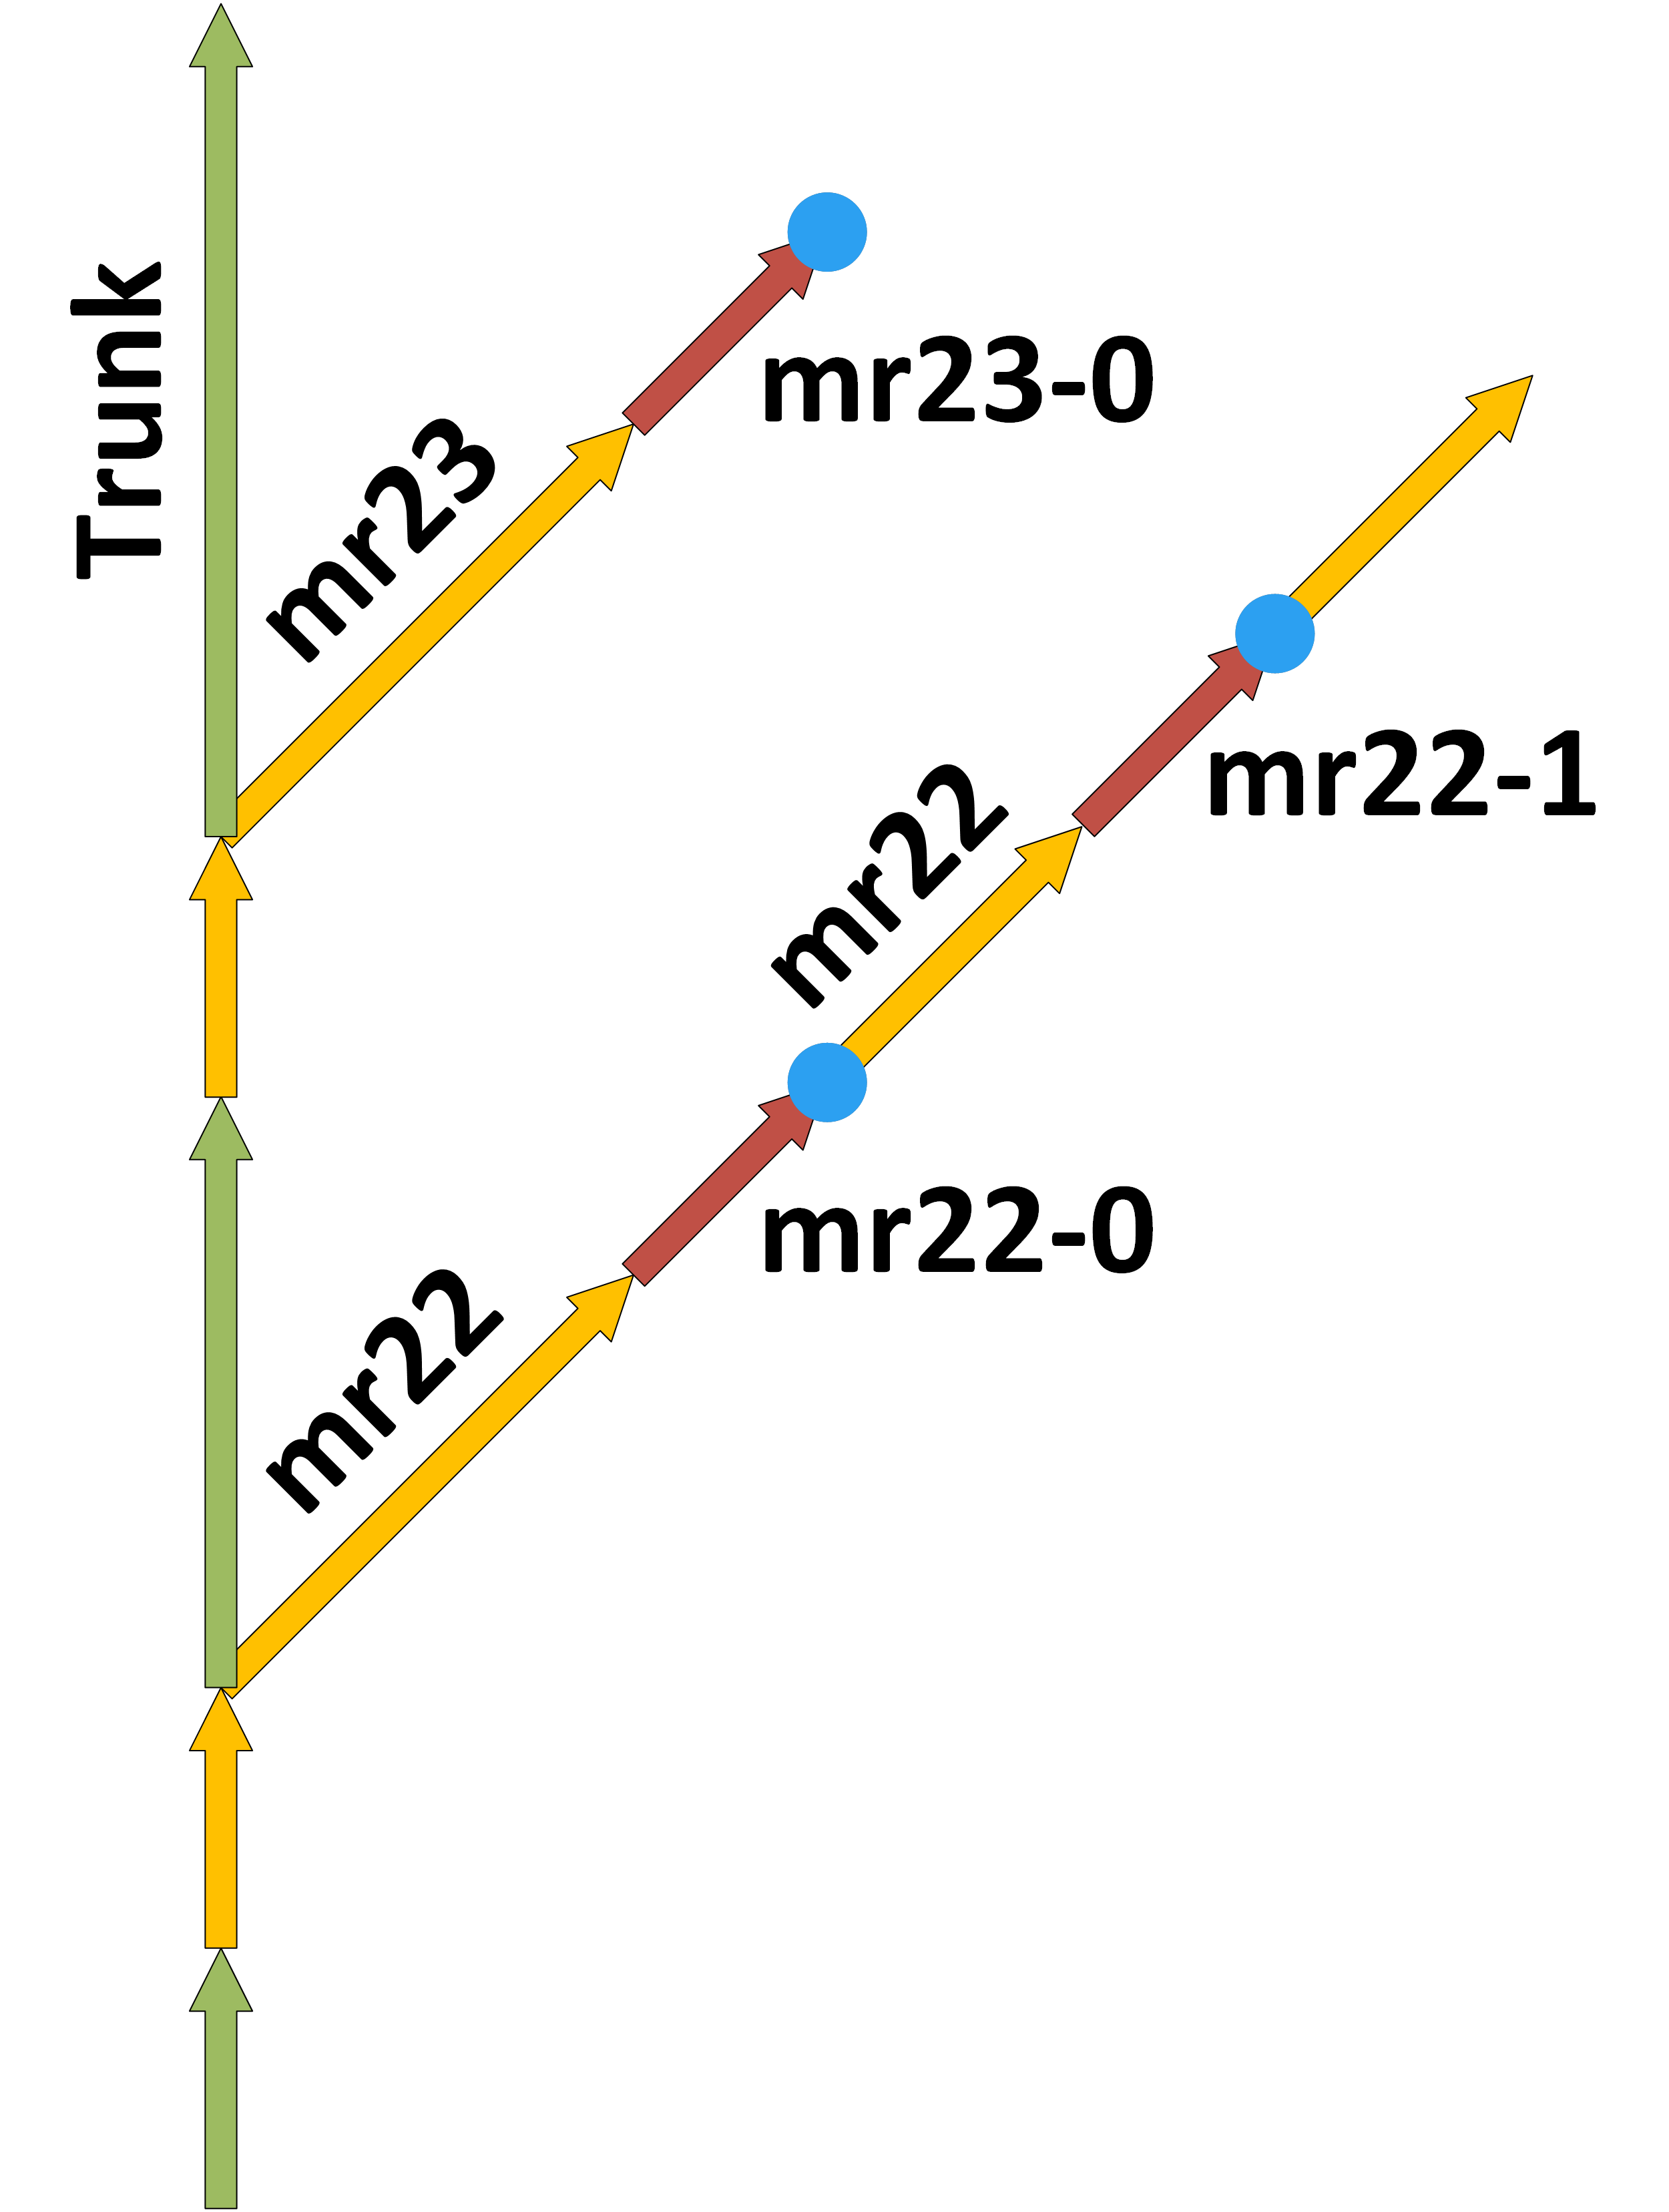
\includegraphics[height=5.5cm]{05_zones_old.png}
\end{figure}



\begin{figure}
  \centering
  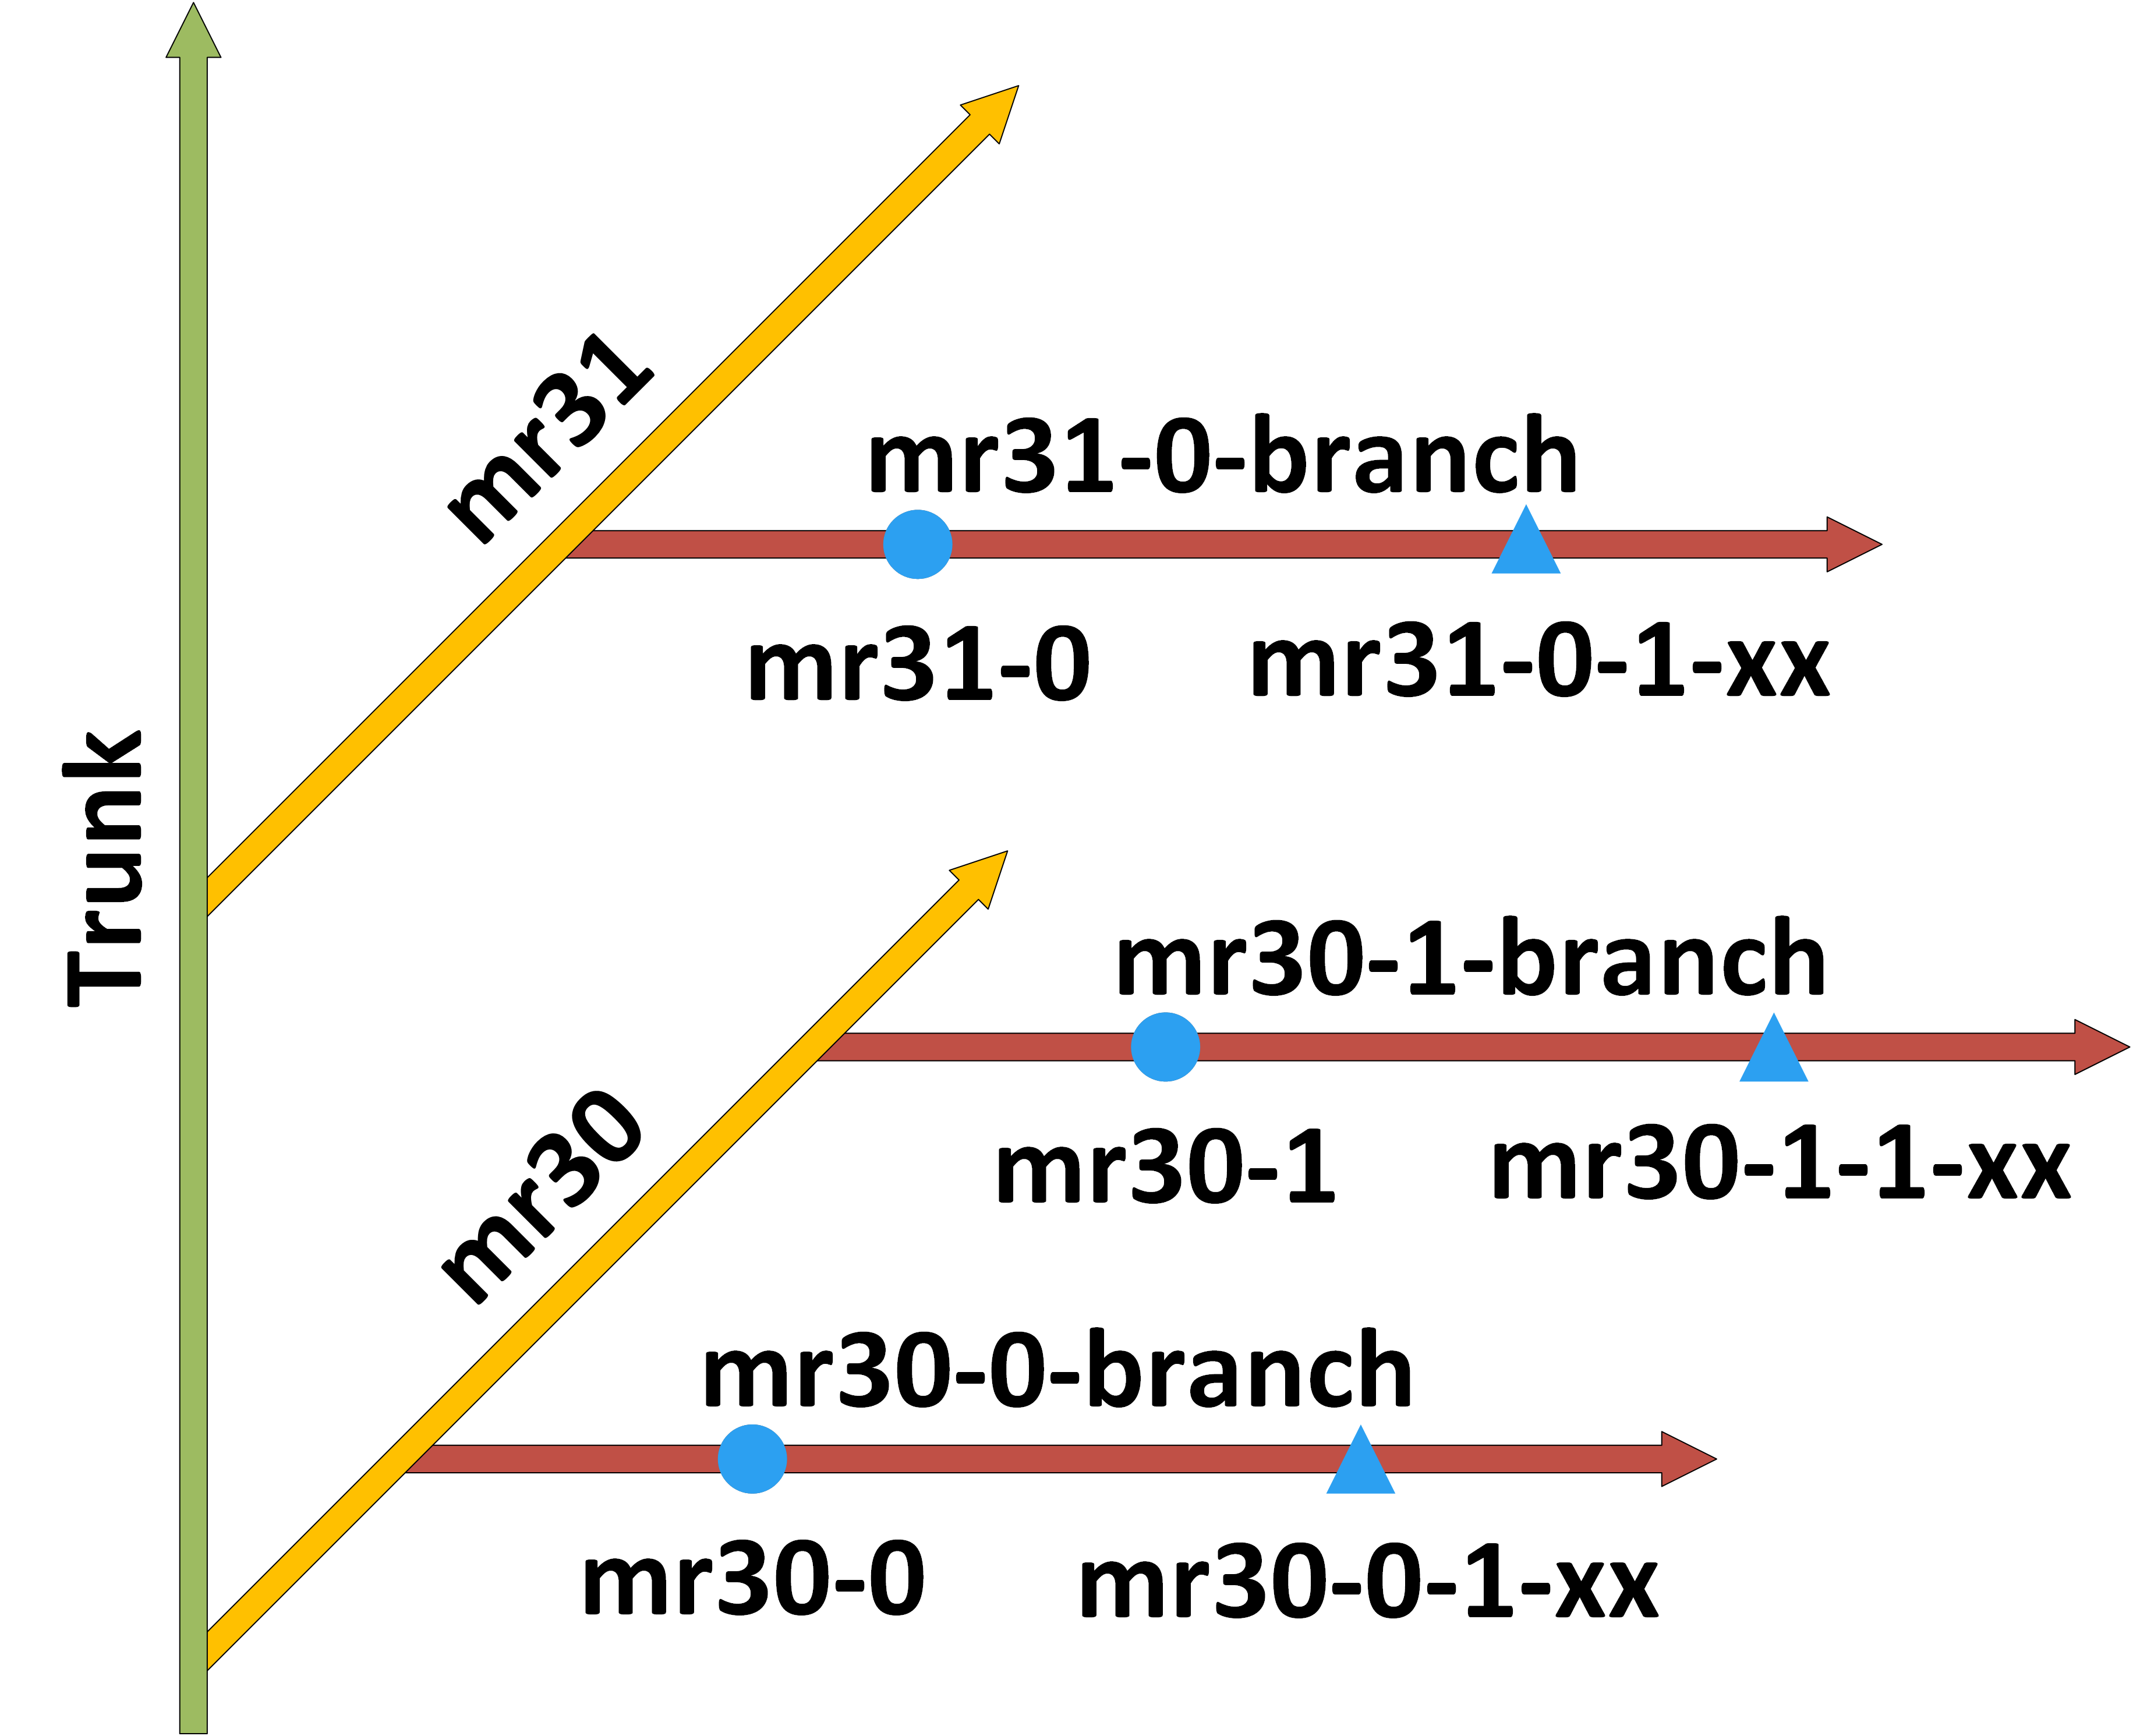
\includegraphics[width=6cm]{05_zones.png}
\end{figure}

Главная ветвь разработки (trunk/master) всегда открыта для приема любых новых функциональных возможностей.

В определенный момент времени (по календарю) от главной ветви <<отщепляется>> новая ветвь, в которой будет проходить стабилизация готовых на тот момент программных возможностей. Эта ветвь сразу становится желтой, т.~е. в неё запрещено добавлять новые возможности, только стабилизировать текущие.

В определенный момент времени от желтой ветви отщепляется красная ветвь. В красную ветвь можно коммитить только по запросу QA отдела.
В определенный момент времени (по календарю), на красной ветви проставляется аннотированная метка (тег) нового релиза.
К этому моменту отдел QA должен завершить тестирование новой версии продукта. Если какие"=то новые программные возможности не готовы и блокируют выпуск новой версии, они должны быть удалены.

Если после проставления аннотированной метки, заказчик или отдел поддержки/эксплуатации находит критический баг, тогда отдел QA запрашивает коммит с исправлением в красную ветвь. После этого на красной ветви проставляется аннотированная метка хотфикса.
Данный подход позволяет разработчикам фиксировать изменения в любой момент времени, потому что главная ветка проекта всегда готова к приему любых изменений, желтые ветки в любой момент готовы к приему исправлений.

\subsection*{Наращивание новых функций и стабильность}

Есть два типа заказчиков: первые хотят стабильности, вторые заказывают новые функциональные возможности и стремятся ими воспользоваться как можно раньше.

Для первого типа заказчиков предлагается раз в год выпускать Long Term Support (LTS) релиз (релиз "--- это нулевой билд, x.0 версия), который будет стабилизироваться в течении года выпуском 6 билдов (версии x.1, x.2 и т.д.) только с исправлениями.
Для второго типа заказчиков предлагается переходить на обычные релизы по мере их выхода. Зачастую в очень сложных проектах новые программные возможности не всегда удовлетворяют заказчика с первого раза. Потому, чаще всего, после сдачи новых возможностей, заказчику нужно немного исправить поведение продукта. Поэтому для каждого обычного релиза выпускается один стабилизационный билд.
Заказчику нужно некоторое время для запуска новой версии продукта в промышленное использование, потому после выхода нового релиза команда разработчиков сразу приступает к выпуску стабилизационного билда к предыдущему релизу. Одновременно с этим разработчики бекпортируют все правки в LTS релиз и выпускают стабилизационный билд для LTS тоже. Т.е. разработчики не ждут отзыва заказчиков, для которых был выпущен новый релиз, а исправляют предыдущий, на который к этому моменту собраны жалобы.

~

\begin{figure}
  \centering
  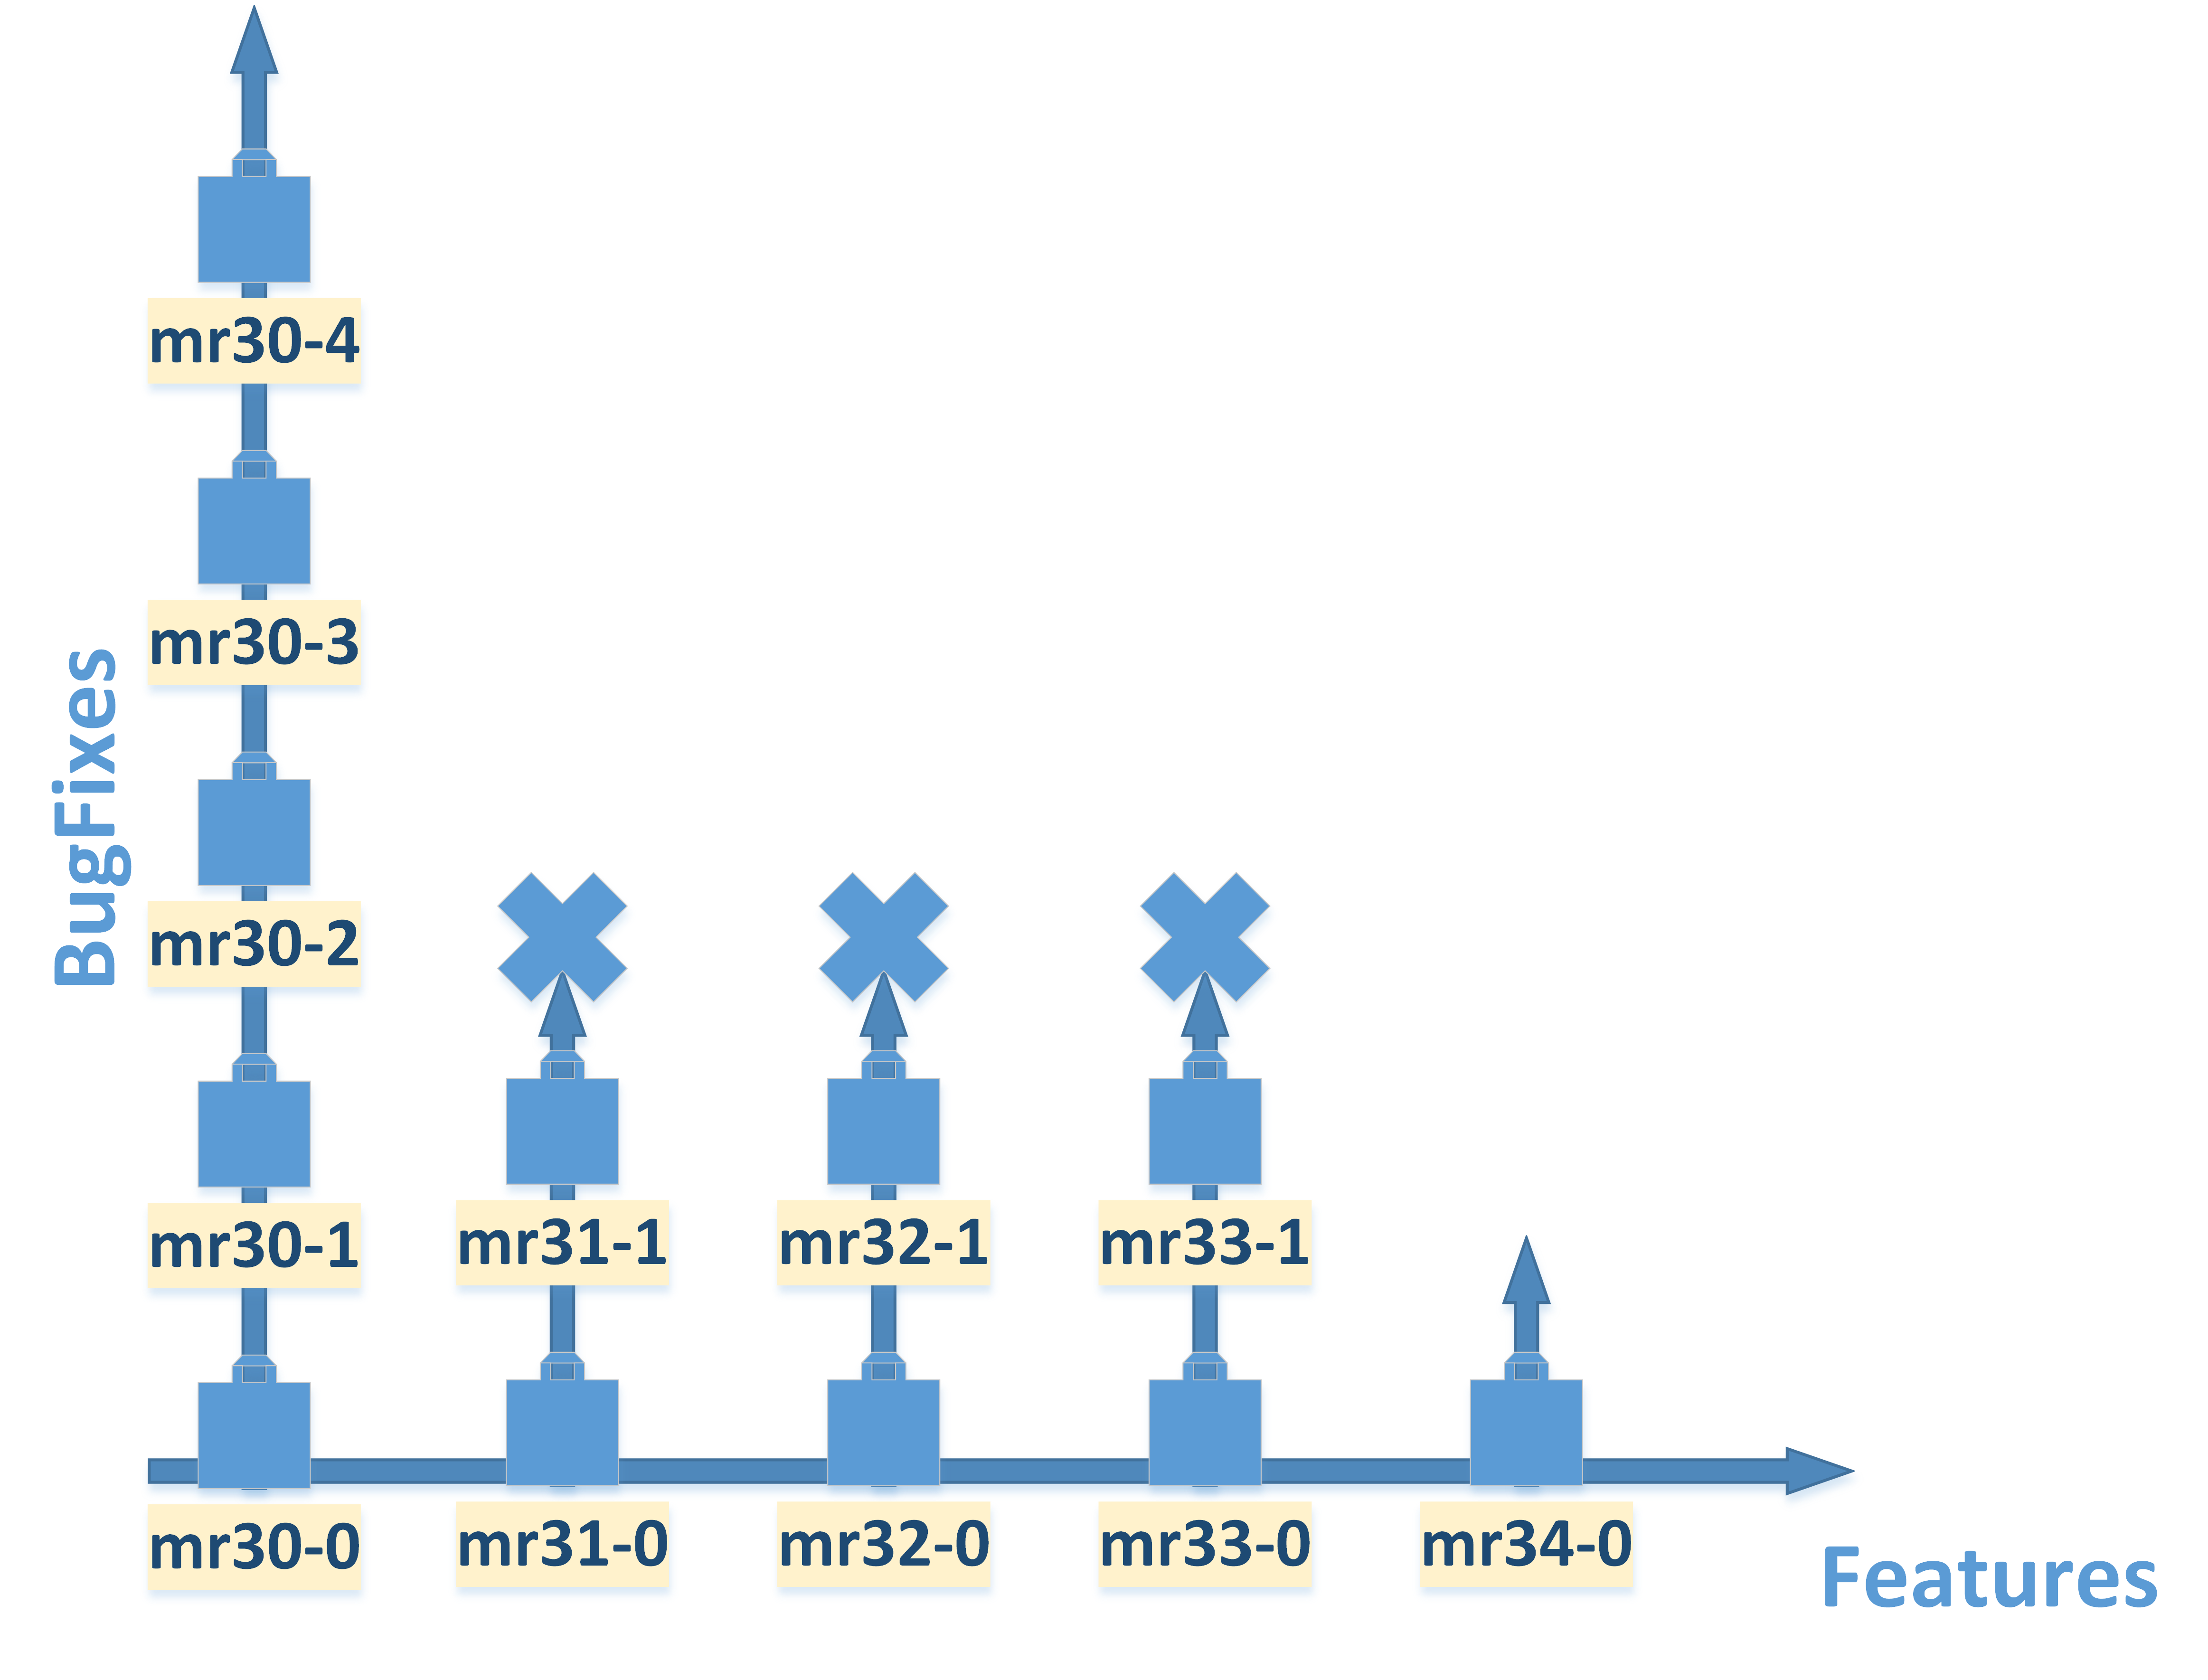
\includegraphics[width=10cm]{05_releases_graph_report.png}
\end{figure}

Данный поход позволяет:

\begin{enumerate}
  \item дать стабильность в LTS релизах;
  \item держать высокий темп выхода новых версий для заказчиков;
  \item продолжать заниматься разработкой, а не ожидать фидбека/багрепортов;
  \item стабилизировать новые версии по мере получения фидбека/багрепортов.
\end{enumerate}

\subsection*{Цикл разработки}

Заказчики хотят получать оплаченные новые возможности точно в срок.
На первый взгляд опыт разработки показывает, что это невозможно. Но это не так. Любые даже самые большие задачи могут быть разбиты на мелкие подзадачи, время на разработку которых возможно подсчитать. При относительно большом цикле (спринте), количество мелких задач, которые могут быть выполнены за определенный срок, стабильно. Не все задачи будут выполнены, но при правильном подсчете этот процент будет мал. В процессе фактической разработки может возникнуть определенное количество новых задач, они тоже должны быть заложены в план. Правильный подсчет времени и количества мелких задач, которые может выполнить отдел разработки в целом,  зависит от грамотности лидеров групп (team lead).

Был предложен следующий цикл разработки:

\begin{figure}[h!]
  \centering
  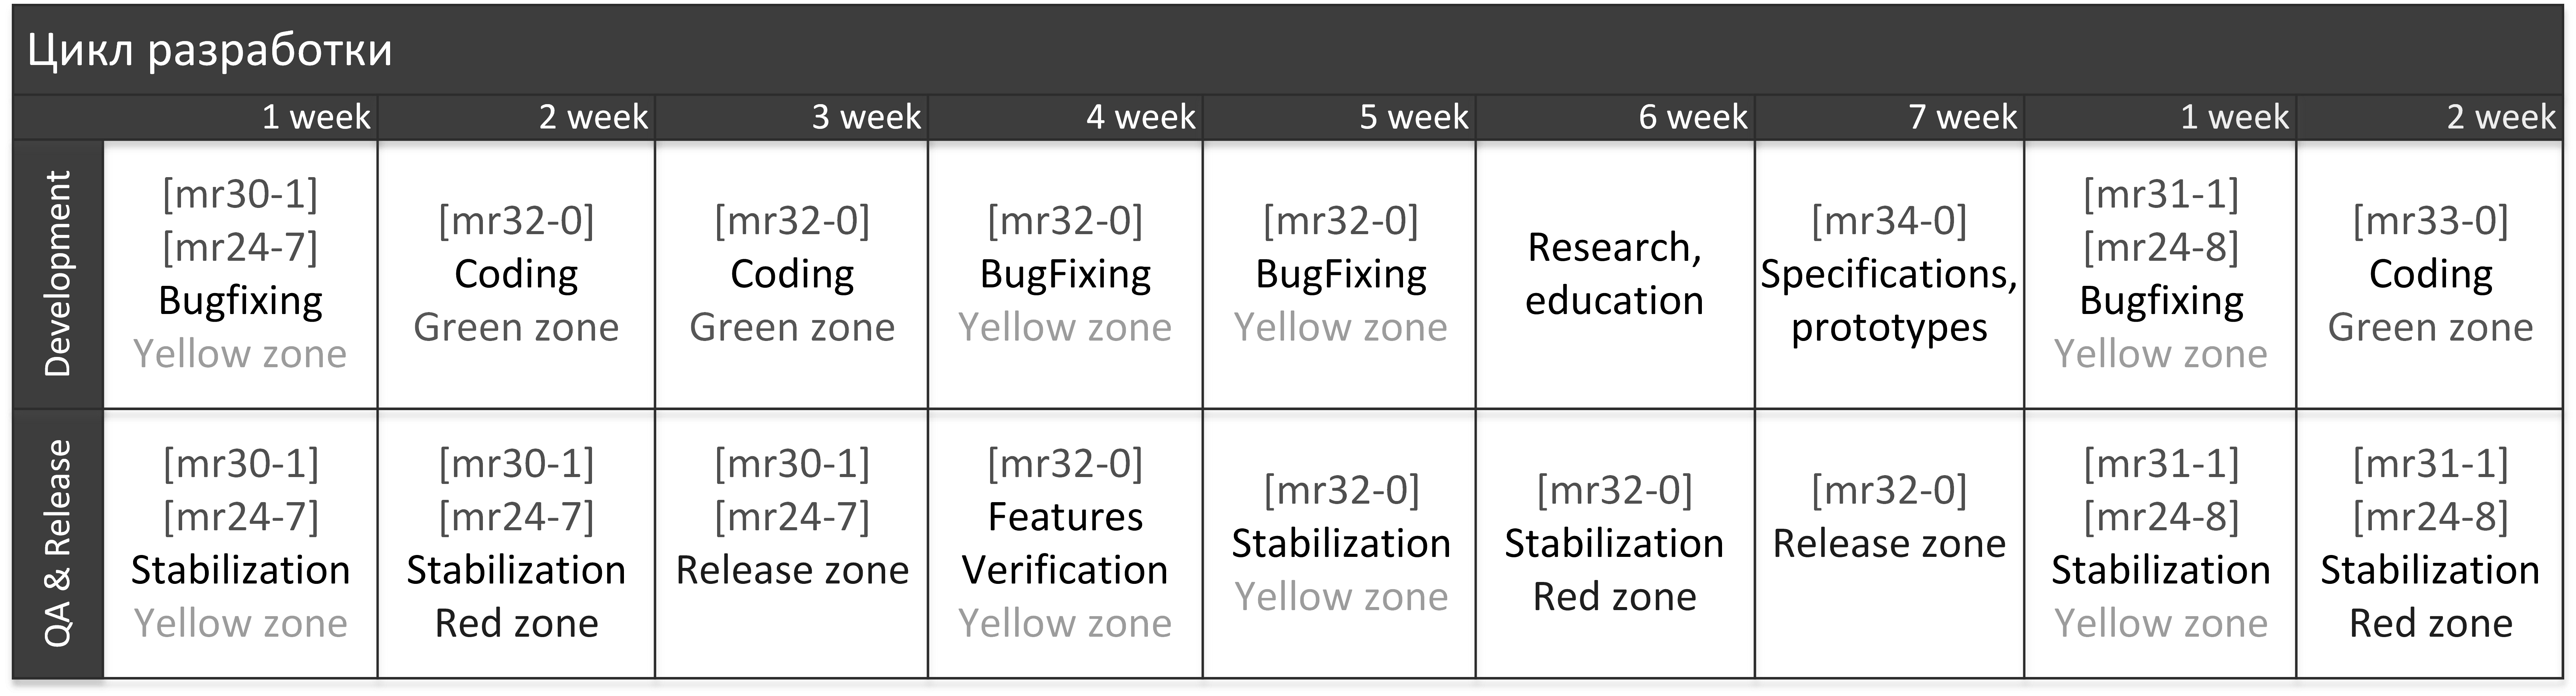
\includegraphics[width=11cm]{05_circle_v3.png}
\end{figure}

\subsection*{Создание спецификаций}

Невозможно гарантировать разработку новых возможностей вовремя, если конечному разработчику не понятны требования заказчика. Потому никакие запросы на новые возможности не будут приняты от заказчика (и не будут названы сроки) пока не будет создана исчерпывающая спецификация, которую примет и заказчик и лидеры групп в отделе разработки. Спецификация должна быть полностью понятна лидерам групп, которые разобьют ее на подзадачи и подсчитают сколько нужно времени на реализацию каждой из них, только после этого заказчику будут названы сроки.

\subsection*{Быстрое развертывание среды разработки}

Используемые OpenSource решения "--- Jenkins, VirtualBox, Vagrant.

Каждому разработчику, что бы начать исправлять ошибку или писать код, нужно иметь личную систему с установленной копией продукта который он разрабатывает. В больших и сложных продуктах довольно долго подготавливать правильно установленный и настроенный продукт (например, базу данных Oracle), это может длиться от нескольких часов до нескольких суток. При высоком темпе выпуска новых версий эта проблема многократно усиливается. Чтобы ускорить процесс развертывания среды разработки был полностью автоматизирован процесс создания образов виртуальных машин для всех версий продукта, для всех платформ с помощью Jenkins CI. Эти образы используются в самом Jenkins для запуска тестов во всех поддерживаемых версиях продукта на всех возможных платформах. С помощью vagrant, гигабитной офисной сети и SSD разработчики могут разворачивать за считанные десятки секунд полностью готовую среду разработки из образа, который имеет актуальный код на нужной платформе.

\subsection*{Автоматизация тестирования}

Используемые OpenSource решения "--- Jenkins.
Код покрыт следующими видами тестов:

\begin{itemize}
  \item Unit test
  \item Functionality test
  \item Performance test
  \item Syntax test
  \item Style test
  \item Code analysis
  \item Compile test
  \item Memory leak test (valgrind)
\end{itemize}

\subsection*{Стабильный транк}

Используемые OpenSource решения "--- Git, Gerrit, gerrit"=tools, Jenkins CI.

~

~

\begin{figure}[b]
  \centering
  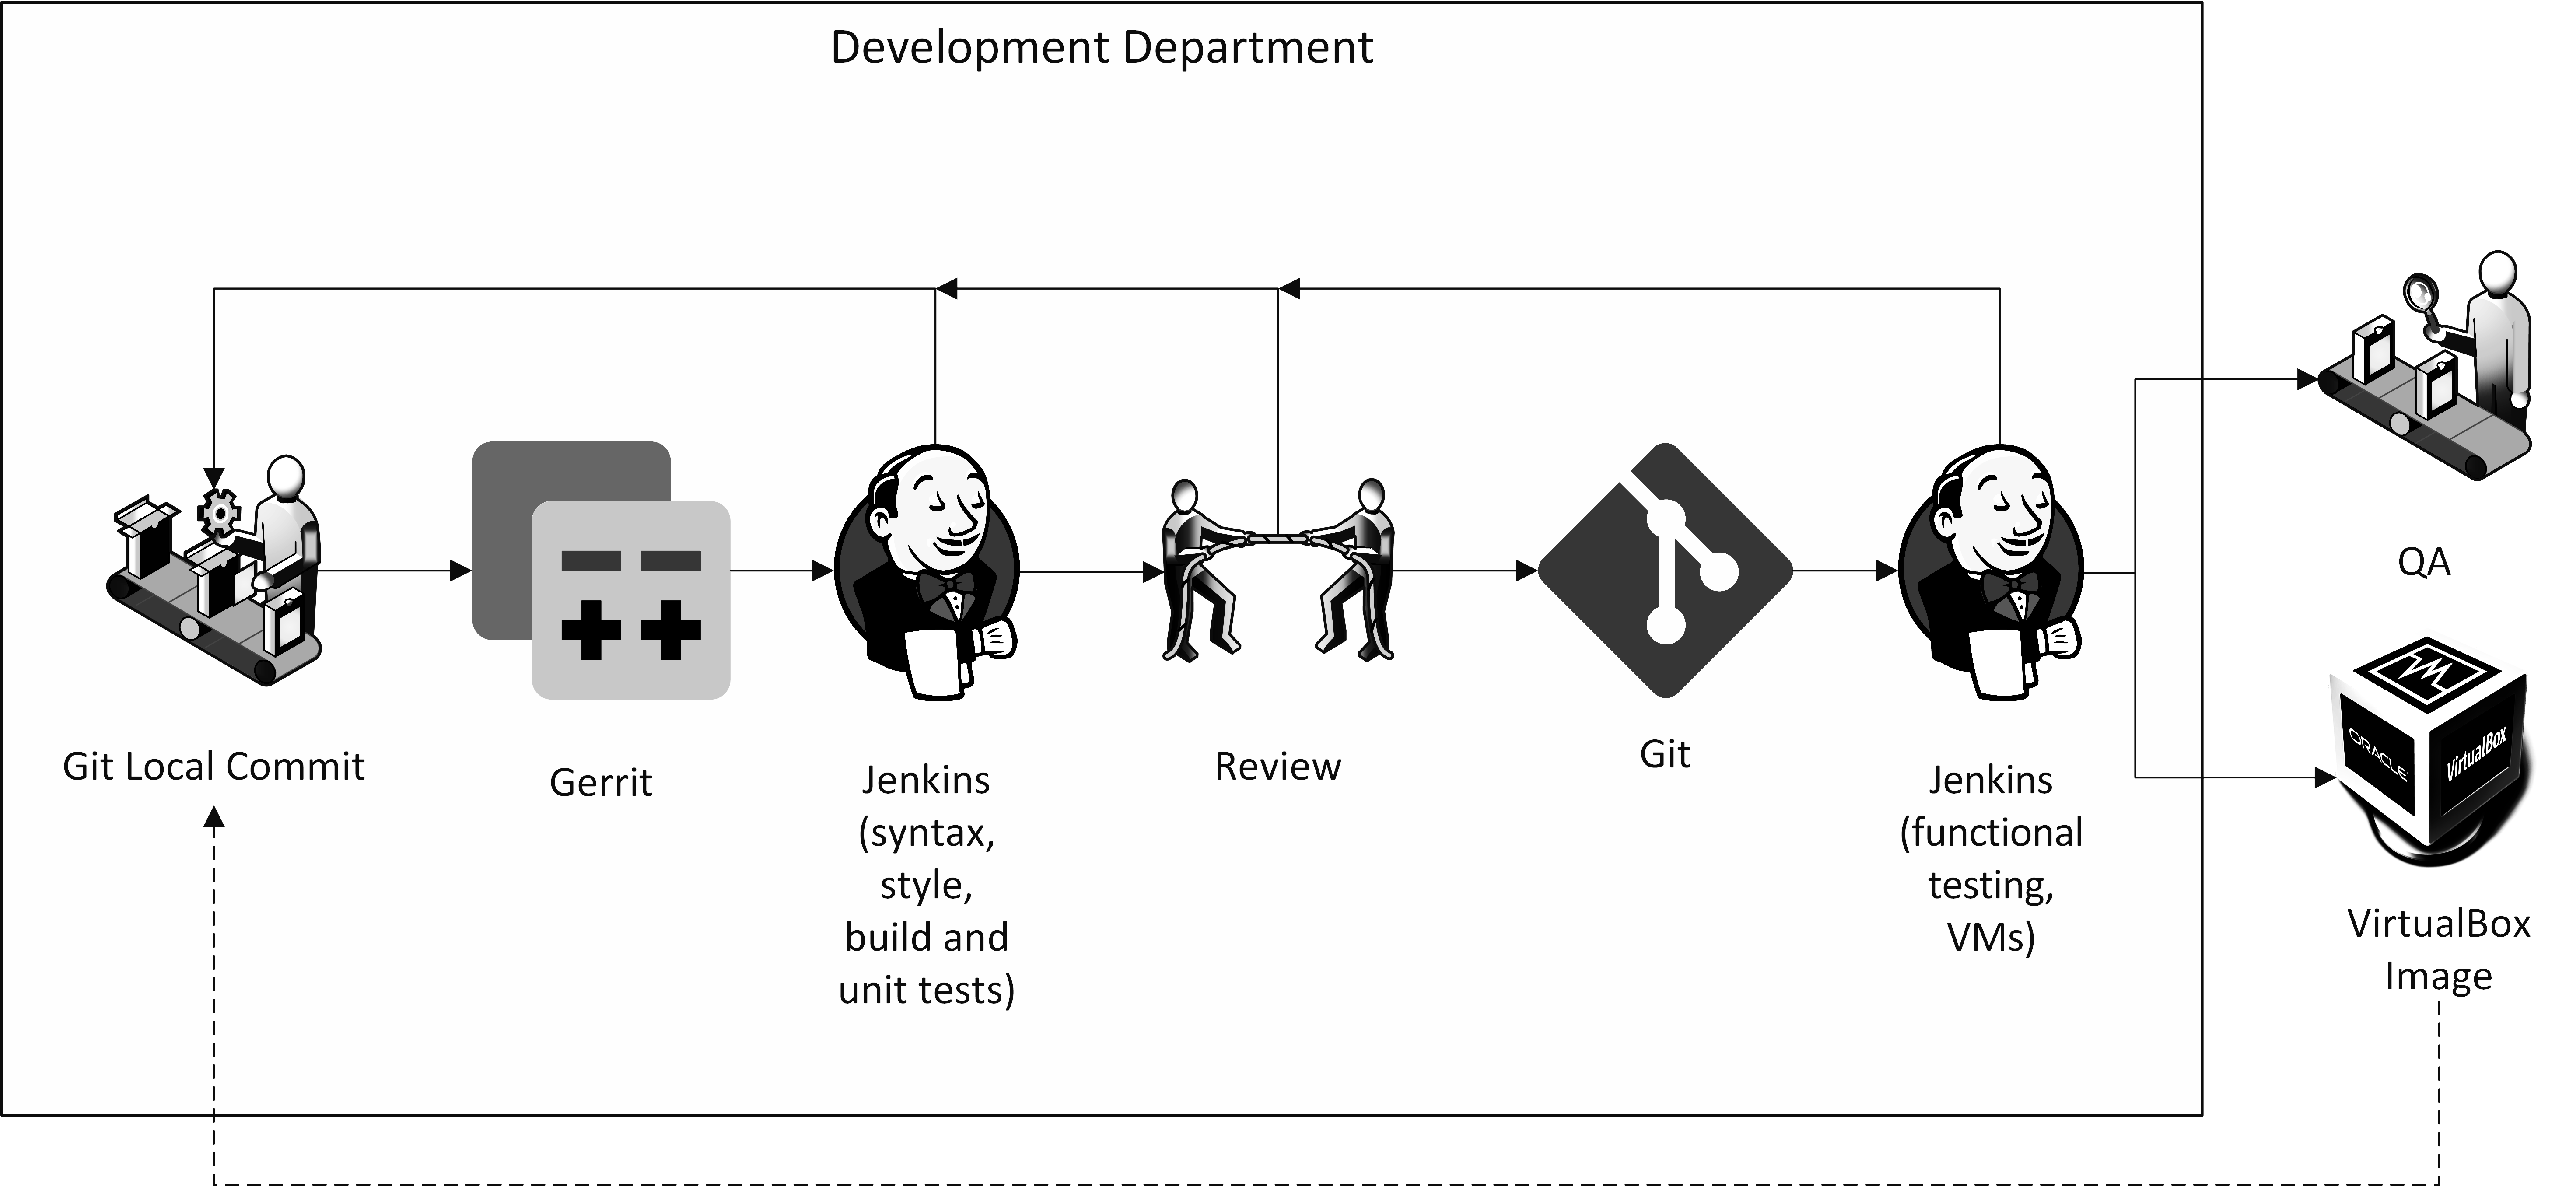
\includegraphics[width=11cm]{05_review.png} 
\end{figure}

Чтобы улучшить стабильность кода, был предложен следующий подход:

\begin{itemize}
  \item разработчик делает фиксацию изменений (коммит) в локальном git репозитории и запускает команду <<git review>>, которая отправляет изменения в gerrit.
  \item Gerrit задерживает изменения, не давая их отправить в центральный репозиторий до тех пор пока изменения не будут проверены рецензентами и автоматическими тестами в Jenkins.
  \item Gerrit тригерит запуск тестов в Jenkins, результат которых выставляется в виде положительной или негативной оценки.
  \item рецензенты могут комментировать код и выставлять оценки от -2 до +2. Код, который не имеет оценки +2 или имеет оценку -2 "--- не может попасть в центральный репозиторий.
  \item когда рецензенты и Jenkins проставили положительные оценки, появляется кнопка <<Submit>> с помощью которой можно пропустить изменения в центральный репозиторий.
  \item раз в день запускаются тяжелые функциональные тесты, которые могут длиться всю ночь.
  \item на основе кода формируются образы виртуальных машин, которые с утра будут загружены разработчиками и QA.
\end{itemize}

\subsection*{Выводы}

Предложенные организационные изменения были проведены в компании PortaOne, Inc. на команде разработчиков из 50 человек и позволили разработчикам больше заниматься любимым делом и выдавать на 30\% больше кода. Отношения с клиентами улучшились благодаря выходу точно в срок новых версий продукта с заказанными функциональными возможностями. Стабильность кода увеличилась за счет введения процедуры review и автоматизации тестирования.


\end{document}





\documentclass[10pt, a5paper]{article}
\usepackage{pdfpages}
\usepackage{parallel}
\usepackage[T2A]{fontenc}
\usepackage{ucs}
\usepackage[utf8x]{inputenc}
\usepackage[polish,english,russian]{babel}
\usepackage{hyperref}
\usepackage{rotating}
\usepackage[inner=2cm,top=1.8cm,outer=2cm,bottom=2.3cm,nohead]{geometry}
\usepackage{listings}
\usepackage{graphicx}
\usepackage{wrapfig}
\usepackage{longtable}
\usepackage{indentfirst}
\usepackage{array}
\newcolumntype{P}[1]{>{\raggedright\arraybackslash}p{#1}}
\frenchspacing
\usepackage{fixltx2e} %text sub- and superscripts
\usepackage{icomma} % коскі ў матэматычным рэжыме
\PreloadUnicodePage{4}

\newcommand{\longpage}{\enlargethispage{\baselineskip}}
\newcommand{\shortpage}{\enlargethispage{-\baselineskip}}

\def\switchlang#1{\expandafter\csname switchlang#1\endcsname}
\def\switchlangbe{
\let\saverefname=\refname%
\def\refname{Літаратура}%
\def\figurename{Іл.}%
}
\def\switchlangen{
\let\saverefname=\refname%
\def\refname{References}%
\def\figurename{Fig.}%
}
\def\switchlangru{
\let\saverefname=\refname%
\let\savefigurename=\figurename%
\def\refname{Литература}%
\def\figurename{Рис.}%
}

\hyphenation{admi-ni-stra-tive}
\hyphenation{ex-pe-ri-ence}
\hyphenation{fle-xi-bi-li-ty}
\hyphenation{Py-thon}
\hyphenation{ma-the-ma-ti-cal}
\hyphenation{re-ported}
\hyphenation{imp-le-menta-tions}
\hyphenation{pro-vides}
\hyphenation{en-gi-neering}
\hyphenation{com-pa-ti-bi-li-ty}
\hyphenation{im-pos-sible}
\hyphenation{desk-top}
\hyphenation{elec-tro-nic}
\hyphenation{com-pa-ny}
\hyphenation{de-ve-lop-ment}
\hyphenation{de-ve-loping}
\hyphenation{de-ve-lop}
\hyphenation{da-ta-ba-se}
\hyphenation{plat-forms}
\hyphenation{or-ga-ni-za-tion}
\hyphenation{pro-gramming}
\hyphenation{in-stru-ments}
\hyphenation{Li-nux}
\hyphenation{sour-ce}
\hyphenation{en-vi-ron-ment}
\hyphenation{Te-le-pathy}
\hyphenation{Li-nux-ov-ka}
\hyphenation{Open-BSD}
\hyphenation{Free-BSD}
\hyphenation{men-ti-on-ed}
\hyphenation{app-li-ca-tion}

\def\progref!#1!{\texttt{#1}}
\renewcommand{\arraystretch}{2} %Іначай формулы ў матрыцы зліпаюцца з лініямі
\usepackage{array}

\def\interview #1 (#2), #3, #4, #5\par{

\section[#1, #3, #4]{#1 -- #3, #4}
\def\qname{LVEE}
\def\aname{#1}
\def\q ##1\par{{\noindent \bf \qname: ##1 }\par}
\def\a{{\noindent \bf \aname: } \def\qname{L}\def\aname{#2}}
}

\def\interview* #1 (#2), #3, #4, #5\par{

\section*{#1\\{\small\rm #3, #4. #5}}

\def\qname{LVEE}
\def\aname{#1}
\def\q ##1\par{{\noindent \bf \qname: ##1 }\par}
\def\a{{\noindent \bf \aname: } \def\qname{L}\def\aname{#2}}
}


\begin{document}

\title{Сеть хранения данных своими руками}%\footnote{Текст данных и последующих тезисов, кроме специально оговоренных случаев, доступен под лицензией Creative Commons Attribution-ShareAlike 3.0}

\author{Роман Шишнев\footnote{Минск, Беларусь; \url{rommer@active.by}}}
\maketitle

\begin{abstract}
There is a small gap in ready solutions between the systems with a local disks and a professional storage systems. The report highlights some technologies and approaches helpful at building personal storage area network of arbitrary size for using in various environments.
\end{abstract}

В настоящее время есть небольшой разрыв между готовыми системами, использующими локальные диски для хранения данных, и профессиональными системами хранения данных. Рассмотрим некоторые современные технологии, которые могут помочь самостоятельно построить сеть хранения данных (СХД) практически любого масштаба для применения в самых различных средах.

На первом шаге постороения личной СХД необходимо определить параметры её производительности и доступность. Ключеными моментами для СХД являются:

\begin{itemize}
  \item объем дискового простанства;
  \item производительность в IOPS (операций ввода-вывода в секунду);
  \item latency (среднее время доступа к данным);
  \item пропускная способность сети;
  \item допустимое время простоя.
\end{itemize}

На обьеме доступного простанства останавливаться не будем, так как тот параметр зависит исключительно от задачи.

Произодительность в количестве операций ввода/вывода в секунду следует рассматривать как ключевой параметр системы. Для примера, один диск SATA с 7200 оборотами в секунду позволяет выполнять около 100 операций при случайном доступе. Именно требуемое количество IOPS для СХД в основном и определяет тип и колическов дисков в нашей системе.

Latency в большей степени также зависит от дисков. Но при достаточно быстрых дисках, например SSD, стоит уже учитывать и задержки, которые возникают в сети при передаче данных.

Пропускная способность сети определяет максимальную скорость, на которой можно будет выполнять операции чтения и записи на системе хранения данных. В зависимости от задачи сеть можно создавать медленном медном гигабитном Ethernet, на 10-ти гигабитной оптике, либо на высокосторостном fiber channel.

Допустимое время простоя определяет количесво дублированных компонентов в сети и системе хранения данных.

Теперь рассмотрим самую простую задачу:

\begin{itemize}
  \item сервер \verb!A!, в котором установлен один SATA"=диск;
  \item сервер \verb!B!, которому нужно получить доступ к этому диску;
  \item гигабитные сетевые карты на каждом из серверов.
\end{itemize}

Для получения доступа к этому диску по сети Ethernet нужно выбрать протокол передачи данных. Самым простым и удобным протоколом в данном случае является iSCSI -- это по сути SCSI"=протокол поверх TCP/IP. На сервер \verb!A! нужно будет установить ПО, которое реализует так называемый iSCSI"=таргет "--- именно он будет осуществлять доступ к диску. На сервере \verb!B! должен быть установлен iSCSI"=инициатор "--- он будет подключаться к дискам. После установки и настройки сервер \verb!B! будет видеть диск сервера \verb!A! так, как будто он локальный.

Добавим в схему сервер \verb!C!, которому также нужен доступ к этому диску.

Для этого схему нужно просто дополнить гигабитным коммутатором, к которому теперь будут подключены все 3 сервера. На сервере \verb!C! достаточно установить / настроить iSCSI"=инициатор и подключить к iSCSI"=таргету на сервере \verb!A!.

После приведенных манипуляций серверы \verb!B! и \verb!C! <<видят>> один и тот же диск.

Имеет смысл предусмотреть также меры по устанению единых точек отказа в системе, и опционально "--- варианты маштабирования системы до десятков и сотен дисков и серверов.

\end{document}





\documentclass[10pt, a5paper]{article}
\usepackage{pdfpages}
\usepackage{parallel}
\usepackage[T2A]{fontenc}
\usepackage{ucs}
\usepackage[utf8x]{inputenc}
\usepackage[polish,english,russian]{babel}
\usepackage{hyperref}
\usepackage{rotating}
\usepackage[inner=2cm,top=1.8cm,outer=2cm,bottom=2.3cm,nohead]{geometry}
\usepackage{listings}
\usepackage{graphicx}
\usepackage{wrapfig}
\usepackage{longtable}
\usepackage{indentfirst}
\usepackage{array}
\newcolumntype{P}[1]{>{\raggedright\arraybackslash}p{#1}}
\frenchspacing
\usepackage{fixltx2e} %text sub- and superscripts
\usepackage{icomma} % коскі ў матэматычным рэжыме
\PreloadUnicodePage{4}

\newcommand{\longpage}{\enlargethispage{\baselineskip}}
\newcommand{\shortpage}{\enlargethispage{-\baselineskip}}

\def\switchlang#1{\expandafter\csname switchlang#1\endcsname}
\def\switchlangbe{
\let\saverefname=\refname%
\def\refname{Літаратура}%
\def\figurename{Іл.}%
}
\def\switchlangen{
\let\saverefname=\refname%
\def\refname{References}%
\def\figurename{Fig.}%
}
\def\switchlangru{
\let\saverefname=\refname%
\let\savefigurename=\figurename%
\def\refname{Литература}%
\def\figurename{Рис.}%
}

\hyphenation{admi-ni-stra-tive}
\hyphenation{ex-pe-ri-ence}
\hyphenation{fle-xi-bi-li-ty}
\hyphenation{Py-thon}
\hyphenation{ma-the-ma-ti-cal}
\hyphenation{re-ported}
\hyphenation{imp-le-menta-tions}
\hyphenation{pro-vides}
\hyphenation{en-gi-neering}
\hyphenation{com-pa-ti-bi-li-ty}
\hyphenation{im-pos-sible}
\hyphenation{desk-top}
\hyphenation{elec-tro-nic}
\hyphenation{com-pa-ny}
\hyphenation{de-ve-lop-ment}
\hyphenation{de-ve-loping}
\hyphenation{de-ve-lop}
\hyphenation{da-ta-ba-se}
\hyphenation{plat-forms}
\hyphenation{or-ga-ni-za-tion}
\hyphenation{pro-gramming}
\hyphenation{in-stru-ments}
\hyphenation{Li-nux}
\hyphenation{sour-ce}
\hyphenation{en-vi-ron-ment}
\hyphenation{Te-le-pathy}
\hyphenation{Li-nux-ov-ka}
\hyphenation{Open-BSD}
\hyphenation{Free-BSD}
\hyphenation{men-ti-on-ed}
\hyphenation{app-li-ca-tion}

\def\progref!#1!{\texttt{#1}}
\renewcommand{\arraystretch}{2} %Іначай формулы ў матрыцы зліпаюцца з лініямі
\usepackage{array}

\def\interview #1 (#2), #3, #4, #5\par{

\section[#1, #3, #4]{#1 -- #3, #4}
\def\qname{LVEE}
\def\aname{#1}
\def\q ##1\par{{\noindent \bf \qname: ##1 }\par}
\def\a{{\noindent \bf \aname: } \def\qname{L}\def\aname{#2}}
}

\def\interview* #1 (#2), #3, #4, #5\par{

\section*{#1\\{\small\rm #3, #4. #5}}

\def\qname{LVEE}
\def\aname{#1}
\def\q ##1\par{{\noindent \bf \qname: ##1 }\par}
\def\a{{\noindent \bf \aname: } \def\qname{L}\def\aname{#2}}
}


\begin{document}

\title{Использование Ejudge для проведения олимпиад по программированию}%\footnote{Текст данных и последующих тезисов, кроме специально оговоренных случаев, доступен под лицензией Creative Commons Attribution-ShareAlike 3.0}

\author{Дмитрий Храбров\footnote{Гомель, Беларусь; ГГТУ им. П.О. Сухого; \url{root@dexp.in}}}
\maketitle

\begin{abstract}
The paper considers usage of open source online programming competitions server ejudge. In addition to technical aspects \linebreak author's personal experience is described, concerning both \linebreak technical and social issues.
\end{abstract}

 Как сказано на официальном сайте, Ejudge "--- это система для проведения различных мероприятий, в которых необходима автоматическая проверка программ. Система может применяться для проведения олимпиад и поддержки учебных курсов. Ejudge распространяется под лицензией GPL, имеет многоязычный веб"=интерфейс и поддерживает защищённое исполнение программ (если установлен патч к ядру Linux). Также система активно используется для проведения олимпиад в различных учебных заведениях, и, по опыту, олимпиады на этой системе проходили успешно.

Для проведения олимпиады необходимо зарегистрировать участников: лично или командно. Далее нужно дать участникам возможность читать условия задач и отправлять решения на тестирование. Перед отсылкой на тестирование участник выбирает компилятор и файл с исходным кодом решения. Далее система на сервере пытается скомпилировать решение с помощью выбранного компилятора. Если произошли ошибки, то участнику выдаётся сообщение. Если компиляция прошла успешно, то происходит непосредственно тестирование. Исполняемому файлу на вход (STDIN или файл) подаются входные данные, заранее сформированные автором задачи. На выполнение обычно ставятся ограничения по времени и по памяти. Если решение участника уложилось в лимиты и выдало ответ, система сверяет этот ответ с авторским. Кроме того система должна вести статистику, показывать положение участников. 

Установка и настройка Ejudge подробно описана на сайте проекта, также есть пошаговые инструкции. Через пакетный менеджер дистрибутива нужно установить необходимые компиляторы, Ejudge при конфигурировании автоматически их подхватит. Так же перед установкой нужно указать пути директорий турниров, веб"=сервера и так далее. После установки надо не забыть запустить демон Ejudge, иначе будет показываться сообщение об ошибке. На случай, если нет желания или возможности выполнять установку и настройку, на официальном сайте лежит готовый и настроенный VirtualBox"=образ.

На официальном сайте Ejudge написано, что она имеет настраиваемый внешний вид. При беглом просмотре такая возможность без перекомпиляции найдена не была. Все страницы свёрстаны абсолютным позиционированием элементов, через CSS трудно поддаются изменениям. Так что мы при использовании системы ограничились заменой логотипа и фона страницы, после чего Ejudge не перестала быть собой в плане не слишком удобного интерфейса, однако стала гораздо более привлекательной.

На текущий момент нами успешно проведена на Ejudge внутривузовская олимпиада по программированию. Наиболее востребованы языки: C\#, Java, C, Pascal. Mono "--- реализация C\# в Linux. Были опасения, что реализация будет отличаться, и студенты будут жаловаться, что C\# не работает. Однако Mono отработало без нареканий. Java поддерживается нативно, однако для этого требуется минимум 512 мегабайт памяти, что необходимо учитывать "--- например, при конфигурировании виртуальной машины. Компиляторов С/С++ нами предоставлялось студентам два: gcc и clang. Студенты периодически путали их и отправляли Си"=программу на тестирование компилятором g++ (для языка С++), однако негативных последствий это не имело. Наибольшее недопонимание вызывало отсутствие заголовочных файлов windows.h и conio.h, которые студенты не задумываясь вставляли в свои программы. Приходилось ходить по аудиториям и повторять, что эти файлы подключать нельзя. Из компиляторов Pascal ограничились Free Pascal, так как этот язык в ВУЗе используется всё меньше; фактически, он был оставлен только для совместимости.

Двое человек спросили о поддержке PHP и Brainfuck. Интерпретатор РНР на сервере установлен и доступен для тестирования приложений. Студенту был предоставлен пример программы, но писать на РНР он не рискнул, так как в аудиториях РНР не установлен. Язык Brainfuck системой Ejudge по умолчанию не поддерживается; студенту пообещали, что язык будет добавлен, если студент гарантирует, что будет на нём писать олимпиаду, после чего вопрос иссяк.

Из неожиданных моментов следует отметить то, что Ejudge по умолчанию считает C\# <<небезопасным>> языком, и он отключен для использования в турнирах. Ещё один тонкий момент был обнаружен после проведения олимпиады "--- система отказалась показать таблицу результатов студентам (пришлось воспользоваться для показа администраторским интерфейсом). Как выяснилось, Ejudge по умолчанию показывает таблицу через 2 часа после завершения олимпиады, однако это настраивается в веб"=интерфейсе.

В целом система тестирования Ejudge показала себя очень неплохо: свою задачу выполняет, поддерживает все современные языки программирования, имеет большое количество настраиваемых возможностей, почти всё доступно через веб"=интерфейс. Из отрицательных черт можно отметить не совсем логичный и удобный интерфейс, причём как турнирный, так и администраторский.


\end{document}





\documentclass[10pt, a5paper]{article}
\usepackage{pdfpages}
\usepackage{parallel}
\usepackage[T2A]{fontenc}
\usepackage{ucs}
\usepackage[utf8x]{inputenc}
\usepackage[polish,english,russian]{babel}
\usepackage{hyperref}
\usepackage{rotating}
\usepackage[inner=2cm,top=1.8cm,outer=2cm,bottom=2.3cm,nohead]{geometry}
\usepackage{listings}
\usepackage{graphicx}
\usepackage{wrapfig}
\usepackage{longtable}
\usepackage{indentfirst}
\usepackage{array}
\newcolumntype{P}[1]{>{\raggedright\arraybackslash}p{#1}}
\frenchspacing
\usepackage{fixltx2e} %text sub- and superscripts
\usepackage{icomma} % коскі ў матэматычным рэжыме
\PreloadUnicodePage{4}

\newcommand{\longpage}{\enlargethispage{\baselineskip}}
\newcommand{\shortpage}{\enlargethispage{-\baselineskip}}

\def\switchlang#1{\expandafter\csname switchlang#1\endcsname}
\def\switchlangbe{
\let\saverefname=\refname%
\def\refname{Літаратура}%
\def\figurename{Іл.}%
}
\def\switchlangen{
\let\saverefname=\refname%
\def\refname{References}%
\def\figurename{Fig.}%
}
\def\switchlangru{
\let\saverefname=\refname%
\let\savefigurename=\figurename%
\def\refname{Литература}%
\def\figurename{Рис.}%
}

\hyphenation{admi-ni-stra-tive}
\hyphenation{ex-pe-ri-ence}
\hyphenation{fle-xi-bi-li-ty}
\hyphenation{Py-thon}
\hyphenation{ma-the-ma-ti-cal}
\hyphenation{re-ported}
\hyphenation{imp-le-menta-tions}
\hyphenation{pro-vides}
\hyphenation{en-gi-neering}
\hyphenation{com-pa-ti-bi-li-ty}
\hyphenation{im-pos-sible}
\hyphenation{desk-top}
\hyphenation{elec-tro-nic}
\hyphenation{com-pa-ny}
\hyphenation{de-ve-lop-ment}
\hyphenation{de-ve-loping}
\hyphenation{de-ve-lop}
\hyphenation{da-ta-ba-se}
\hyphenation{plat-forms}
\hyphenation{or-ga-ni-za-tion}
\hyphenation{pro-gramming}
\hyphenation{in-stru-ments}
\hyphenation{Li-nux}
\hyphenation{sour-ce}
\hyphenation{en-vi-ron-ment}
\hyphenation{Te-le-pathy}
\hyphenation{Li-nux-ov-ka}
\hyphenation{Open-BSD}
\hyphenation{Free-BSD}
\hyphenation{men-ti-on-ed}
\hyphenation{app-li-ca-tion}

\def\progref!#1!{\texttt{#1}}
\renewcommand{\arraystretch}{2} %Іначай формулы ў матрыцы зліпаюцца з лініямі
\usepackage{array}

\def\interview #1 (#2), #3, #4, #5\par{

\section[#1, #3, #4]{#1 -- #3, #4}
\def\qname{LVEE}
\def\aname{#1}
\def\q ##1\par{{\noindent \bf \qname: ##1 }\par}
\def\a{{\noindent \bf \aname: } \def\qname{L}\def\aname{#2}}
}

\def\interview* #1 (#2), #3, #4, #5\par{

\section*{#1\\{\small\rm #3, #4. #5}}

\def\qname{LVEE}
\def\aname{#1}
\def\q ##1\par{{\noindent \bf \qname: ##1 }\par}
\def\a{{\noindent \bf \aname: } \def\qname{L}\def\aname{#2}}
}


\begin{document}

\title{pkgsrc4unix}%\footnote{Текст данных и последующих тезисов, кроме специально оговоренных случаев, доступен под лицензией Creative Commons Attribution-ShareAlike 3.0}

\author{Алексей Чеусов\footnote{Минск, Беларусь;\url{vle@gmx.net}}}
\maketitle

\begin{abstract}
pkgsrc is a cross"=platform packaging system. Besides NetBSD where it was born in 1997, pkgsrc supports Linux, Solaris, all BSDs, Minix, QNX and a lot of others. In total 15 platforms are supported. Pkgsrc has a number of advantages over existing packaging systems: easy packaging, support for many compilers, efficient binary package management and source"=based upgrades but the killer"=feature is a support for diverse operating systems. Adapting pkgsrc for Linux as an additional yum/zypper/apt repository of binary packages is considered here.
\end{abstract}

pkgsrc --- кросс"=платформная пакетная система, созданная в 1997 году как ответвление FreeBSD ports. Несмотря на то, что разрабатывается она в основном разработчиками NetBSD, pkgsrc поддерживает практически все живые операционные системы, существующие на данный момент. Среди них Linux, Solaris, все варианты BSD, QNX, Haiku, AIX, HP"=UX и многие другие. pkgsrc является по сути единственной пакетной системой, поддерживающей на неплохом уровне такой широкий набор операционных систем, что дает пользователю, будь то крупная компания или один человек, возможность на любой платформе использовать один и тот же знакомый набор пакетов для работы. Это очень удобно особенно в тех случаях, когда пользователю необходимо достаточно редкое программное обеспечение, отсутствующее по той или иной причине в типичных, в последнее время Десктоп"=ориентированных, Линукс"=истрибутивах.

В подобных случаях есть два принципиально разных пути решения этой проблемы. Путь первый --- если пакета нет в системе, значит он нам не нужен (однако это неподходящий метод). Второй путь --- самостоятельное пакетирование. Опытный специалист в состоянии самостоятельно запакетировать необходимое ПО под необходимый дистрибутив или систему. В этом случае требуется изучить правила пакетирования для конкретной системы и строго следовать им. На мой взгляд, с этим связан один существенный недостаток. Эти правила часто весьма специфичны, а полученные от их изучения знания лишь отчасти могут быть применены при работе с другими системами. Так, например, диалекты rpm spec и доступный набор макроопределений довольно сильно отличаются в различных дистрибутивах Линукс и практически не используются в других ОС, а правила пакетирования для OpenBSD, FreeBSD, Gentoo или Arch linux вообще мало похожи на остальные системы пакетирования. Другой недостаток, еще более серьезный --- это ориентированность разработанного пакета на одну определенную систему, а чаще всего, дистрибутив. Если выбор ОС и дистрибутива уже сделан, и сделан на всю жизнь, это не представляет большой проблемы, но едва ли найдется достаточно много людей, осознанно использующих одну единственную систему более, скажем, пяти лет. Обычно система подбирается под конкретную решаемую задачу, а не наоборот, поэтому часто складывается ситуация, когда система уже определена, а потому усилия потраченные на самостоятельное пакетирование необходимого ПО под другую систему могут оказаться напрасными. Частично эту проблему решает система OpenBuildService (OBS), разрабатываемая сообществом OpenSuSE. Она позволяет, имея в распоряжении единый язык для описания сценариев пакетирования (rpm spec) создать пакет для различных дистрибутивов Линукс. Но\ldots{} только Линукса! Инфраструктура инфтраструктурой, но для успешного пакетирования тысяч и тысяч пакетов под различные операционные системы и среды необходимо сообщество, в котором уже сложилась традиция разработки переносимого ПО. Едва ли Линукс"=сообщество в целом и сообщество OpenSuSE/OBS в частности на это способно. Скорее наоборот, в последнее время все чаще в мире Linux раздаются призывы отказаться от POSIX и разработывать ПО исключительно под единственно"=верную систему.

К счастью, не все разработчики забыли о пользе переносимости. Одно из сообществ таких разработчиков --- разработчики pkgsrc, где, как уже было сказано, пакеты изначально разрабатываются с расчетом на то, чтобы обеспечить максимально возможное количество поддержиаемых систем. pkgsrc обладает всем необходимым для серьезной работы: удобным механизмом сборки пакетов, включая разработку заплаток для исправления ошибок, поддержкой работы с бинарными пакетами, системой массовой сборки пакетов (bulk builders) и прочим. По ряду параметров pkgsrc превосходит форматы rpm и deb и соответствующие программы (dpkg, yum, apt, zypper и т.д.), наиболее широко используемые в Линукс и считающиеся стандартом de facto. 

Из коробки pkgsrc предоставляет весь необходимый набор инструментов как для разработки и сборки пакетов, так и для управления установленными пакетами в системе. С точки зрения системного администратора pkgsrc в системе будет иметь отдельную базу данных установленных пакетов (pkgdb) параллельно с основной использующейся в системе, например, rpmdb и, соответственно, отдельный набор пакетов и утилит для работы с ними. Будучи небольшой проблемой для профессионала, это может оказаться неудобным для массового пользователя. Один из способов решения данной проблемы --- преобразование <<родных>> пакетов pkgsrc в <<родные>> пакеты системы, формирование на их основе репозитория дополнительного ПО и установка/удаление/поиск/\ldots{} по общим для системы правилам, будь то yum, zypper или aptitude.

Цель моего собственного проекта pkgsrc4unix --- создание регулярно обновляемого полноценного yum"=репозитория пакетов для RHEL"=6 (для начала), создаваемого на основе pkgsrc. Его особенности: 
\begin{itemize}
\item для сборки ПО используется инфраструктура pkgsrc, а не rpm spec; 
\item для массовой сборки пакетов также используются средства pkgsrc; 
\item пакеты в формате pkgsrc преобразуются в .rpm для RHEL"=6 и далее из rpm"=пакетов создается yum"=репозиторий; 
\item для исключения конфликтов на уровне файлов с пакетами RHEL, repoforge, epel и др. все ПО устанавливается в \linebreak /opt/pkgsrc4unix, для исключения конфликтов на уровне названий пакетов каждый пакет имеет префикс <<nb->>; 
\item для управления конфигурационными файлами используется подход pkgsrc; 
\item для старта демонов используется механизм NetBSD/pkgsrc, при этом все необходимое для этого ПО реализуется в виде отдельного rpm"=пакета.
\end{itemize}



\end{document}





\documentclass[10pt, a5paper]{article}
\usepackage{pdfpages}
\usepackage{parallel}
\usepackage[T2A]{fontenc}
\usepackage{ucs}
\usepackage[utf8x]{inputenc}
\usepackage[polish,english,russian]{babel}
\usepackage{hyperref}
\usepackage{rotating}
\usepackage[inner=2cm,top=1.8cm,outer=2cm,bottom=2.3cm,nohead]{geometry}
\usepackage{listings}
\usepackage{graphicx}
\usepackage{wrapfig}
\usepackage{longtable}
\usepackage{indentfirst}
\usepackage{array}
\newcolumntype{P}[1]{>{\raggedright\arraybackslash}p{#1}}
\frenchspacing
\usepackage{fixltx2e} %text sub- and superscripts
\usepackage{icomma} % коскі ў матэматычным рэжыме
\PreloadUnicodePage{4}

\newcommand{\longpage}{\enlargethispage{\baselineskip}}
\newcommand{\shortpage}{\enlargethispage{-\baselineskip}}

\def\switchlang#1{\expandafter\csname switchlang#1\endcsname}
\def\switchlangbe{
\let\saverefname=\refname%
\def\refname{Літаратура}%
\def\figurename{Іл.}%
}
\def\switchlangen{
\let\saverefname=\refname%
\def\refname{References}%
\def\figurename{Fig.}%
}
\def\switchlangru{
\let\saverefname=\refname%
\let\savefigurename=\figurename%
\def\refname{Литература}%
\def\figurename{Рис.}%
}

\hyphenation{admi-ni-stra-tive}
\hyphenation{ex-pe-ri-ence}
\hyphenation{fle-xi-bi-li-ty}
\hyphenation{Py-thon}
\hyphenation{ma-the-ma-ti-cal}
\hyphenation{re-ported}
\hyphenation{imp-le-menta-tions}
\hyphenation{pro-vides}
\hyphenation{en-gi-neering}
\hyphenation{com-pa-ti-bi-li-ty}
\hyphenation{im-pos-sible}
\hyphenation{desk-top}
\hyphenation{elec-tro-nic}
\hyphenation{com-pa-ny}
\hyphenation{de-ve-lop-ment}
\hyphenation{de-ve-loping}
\hyphenation{de-ve-lop}
\hyphenation{da-ta-ba-se}
\hyphenation{plat-forms}
\hyphenation{or-ga-ni-za-tion}
\hyphenation{pro-gramming}
\hyphenation{in-stru-ments}
\hyphenation{Li-nux}
\hyphenation{sour-ce}
\hyphenation{en-vi-ron-ment}
\hyphenation{Te-le-pathy}
\hyphenation{Li-nux-ov-ka}
\hyphenation{Open-BSD}
\hyphenation{Free-BSD}
\hyphenation{men-ti-on-ed}
\hyphenation{app-li-ca-tion}

\def\progref!#1!{\texttt{#1}}
\renewcommand{\arraystretch}{2} %Іначай формулы ў матрыцы зліпаюцца з лініямі
\usepackage{array}

\def\interview #1 (#2), #3, #4, #5\par{

\section[#1, #3, #4]{#1 -- #3, #4}
\def\qname{LVEE}
\def\aname{#1}
\def\q ##1\par{{\noindent \bf \qname: ##1 }\par}
\def\a{{\noindent \bf \aname: } \def\qname{L}\def\aname{#2}}
}

\def\interview* #1 (#2), #3, #4, #5\par{

\section*{#1\\{\small\rm #3, #4. #5}}

\def\qname{LVEE}
\def\aname{#1}
\def\q ##1\par{{\noindent \bf \qname: ##1 }\par}
\def\a{{\noindent \bf \aname: } \def\qname{L}\def\aname{#2}}
}


\begin{document}

\switchlang{be}
\title{Алгарытмы паляпшэння выяваў у ВПЗ: падвышэнне рэзкасці}%\footnote{Текст данных и последующих тезисов, кроме специально оговоренных случаев, доступен под лицензией Creative Commons Attribution-ShareAlike 3.0}

\author{Антон Літвіненка\footnote{Кіеў, Украіна; \url{tenebrosus.scriptor@gmail.com}. Пашыраная версія артыкула з прыкладамі апрацоўкі: \url{http://lvee.org/be/abstracts/76}}}
\maketitle

\begin{abstract}
A review of image sharpening enhancement algorithms devilered by FLOSS projects is provided together with discussion of their end-user characteristics and some theoretical aspects.
\end{abstract}

Крыніцы нярэзкасці ў выяве:
\begin{itemize}
  \item Памылка факусіроўкі;
  \item Нізкая якасць/«мяккасць» аб’ектыва;
  \item Характарыстыкі планшэтных сканэраў;
  \item Дрыжанне рук (у цемры) ці іншыя прычыны руху здымача;
\end{itemize}

Далей будзе разгледжаны шэраг алгарытмаў для выдалення шумоў з выявы і іх рэалізацыю ў вольных праграмных прадуктах: \href{http://www.gimp.org/}{GIMP} (GPL3+), \href{http://www.imagemagick.org/}{ImageMagick} (Apache 2.0), \href{http://gmic.sourceforge.net/}{G’MIC} (CeCILL license), \href{http://krita.org/}{Krita} (GPL2).

\paragraph*{USM.} Unsharp mask, альбо маска нярэзкасці. Алгарытм: змешванне выявы з яе гаўсавым размыццём. Наяўная амаль ва ўсіх рэдактарах, якія заяўляюць магчымасць апрацоўкі выяваў (нават пры аптычным друку здымкаў з плёнак) — {GIMP}, {ImageMagick}, {Krita}, {G'MIC}.

Перавагі:

\begin{itemize}
  \item Універсальнасць і распаўсюджанасць;
  \item Магчымасць застасавання парогу (рэзкасць павялічваецца толькі для тых фрагментаў выявы, якія адрозніваюцца ад навакольных на пэўную парогавую велічыню (застасоўваецца селектыўнае гаўсава размыццё);
\end{itemize}

Недахопы:

\begin{itemize}
  \item Нізкая сэлектыўнасць, не ўлічваецца марфалогія выявы;
  \item Метад накіраваны не на кампенсацыю эфектаў, якія прывялі да нярэзкасці, а на візуальнае успрыняцце здымку як больш рэзкага;
  \item Пры моцным павялічэнні рэзкасці каля краёў выявы з’яўляюцца артэфакты.
\end{itemize}

\paragraph*{Алгарытмы, заснаваныя на аналізе марфалогіі.} Шэраг метадаў, якія шукаюць контуры на выяве і імкнуцца падвысіць рэзкасць контуру, не кранаючы абласцей павольнага пераходу значэнняў пікселаў.

Рэалізацыі:
\begin{itemize}
  \item ImageMagick (складанне выявы з вынікам працы аналізатара марфалогіі LoG (лапласіян гаўсіяна)\cite{litv1})
\texttt{convert 1.png -define convolve:scale='100,100\%' -morphology Convolve 'Log:0x2' 1\_sharpen.png}
\end{itemize}

\begin{itemize}
  \item GIMP-плагін «erosion sharpening» (змешванне выявы з вынікамі застасавання да яе аперацый «dilate» ды «erode»).
\end{itemize}

Перавагі:
\begin{itemize}
  \item Больш селектыўныя ў параўнанні з USM.
\end{itemize}

Недахопы:
\begin{itemize}
  \item Складаней застасаваць парогавае значэнне, таму разам з рэзкасцю павялічваюць шум (патрабуе папярэдняга падаўлення шуму).
\end{itemize}

\paragraph*{Wavelet.} Алгарытм, у нечым падобны на папярэдні, дзе для выдзялення краёў ужываюцца вэйвлеты. Выконваецца вэйвлетны расклад выявы, і ўзмацняюцца некаторыя ягоныя складнікі.

Рэалізацыя: плагін для GIMP.

Перавагі:

\begin{itemize}
  \item Адзін з найбольш эфектыўных метадаў падвышэння рэзкасці;
  \item Можа ўжывацца разам з вэйвлетным падаўленнем шумоў (камбінаванне двух застасаванняў вэйвлетнага раскладу дае неблагія вынікі);
\end{itemize}

Недахопы:

\begin{itemize}
  \item Немагчыма застасаванне парогу.
\end{itemize}

\paragraph*{Алгарытмы, заснаваныя на пошуку ці ўгадванні функцыі распаўсюджання кропкі.}

Прычыны, якія выклікаюць размыццё выявы, маюць як стахастычную частку (якая вызначаецца выпадковымі дэфектамі, разбалансіроўкай частак аптычнае схемы, ці проста ўкладам шумоў) і функцыянальна-заканамерную (напрыклад, у выпадку размыцця рухам ці памылкі факусіроўкі значэнні пікселаў выніковай выявы знаходзяцца ў функцыянальнай залежнасці ад значэнняў пікселаў арыгінальнай). У выпадку, калі функцыянальна-заканамернае размыццё дамінуе (альбо калі такую функцыянальную залежнасць можна знайсці), веданне дакладнай функцыі размеркавання кропкі (PSF, point spread function) тэарэтычна дазваляе цалкам аднавіць арыгінальную выяву (з агаворкамі наконт краёў).

На практыцы ідэальнаму аднаўленню замінае брак ведаў дакладнай PSF і шум. Тым не менш, існуе шэраг рэалізацый, якія тым ці іншым спосабам імкнуцца ацаніць PSF (кіруючыся пэўнымі меркаваннямі наконт прычыны размыцця ці з агульных меркаванняў), і з меншым ці большым поспехам аднавіць выяву.

\begin{itemize}
  \item Deconvolution sharpening у {G'MIC} (алгарытм Рычардсана-Люсі \cite{litv2});
  \item Плагін Refocus у {GIMP} (алгарытм Вінера \cite{litv3}) — расфакусіроўка etc.;
  \item Refocus-it у {GIMP} (нэйронная сетка Хопфілда \cite{litv4}) — расфакусіроўка, размыццё рухам, гаўсава размыццё;
\end{itemize}

Перавагі:

\begin{itemize}
  \item Скіраваныя на тое, каб прыбраць прычыны ўзнікнення нярэзкасці;
  \item Могуць дазволіць выцягнуць інфармацыю з выявы там, дзе іншыя метады няздольныя нават тэарэтычна;
\end{itemize}

Недахопы:

\begin{itemize}
  \item Патрабуюць шмат вылічальных рэсурсаў;
  \item Часта атрымліваюцца выявы са скажэннямі.
\end{itemize}

Паводле асабістага досведу аўтар можа рэкамендаваць выкарыстанне вэйвлетнага алгарытму ў абсалютнай большасці выпадкаў.

Такім чынам, вольнае праграмнае забеспячэнне надае шырокі спектр магутных тэарэтычна абгрунтаваных алгарытмаў падвышэння рэзкасці выяваў, якія грунтуюцца як на візуальным падвышэнні рэзкасці, так і на супрацьдзеянні фізічным прычынам, якія вядуць да яе зніжэння. У адрозненне ад алгарытмаў падаўлення шумоў, алгарытмы падвышэння рэзкасці заўважна адрозніваюцца ад праграмы да праграмы і ў асноўным рэалізаваныя як плагіны альбо скрыпты. Дакладным лідэрам у колькасці рэалізаваных алгарытмаў з’яўляецца {GIMP} (асабліва калі браць да ўвагі {G'MIC} for {GIMP}).

\begin{thebibliography}{9}
\bibitem{litv1} \url{http://www.imagemagick.org/Usage/convolve/#sharpen}
\bibitem{litv2} JOSA, 62, 1, pp. 55-59 (1972); Astronomical Journal, 79, p. 745 (1974).
\bibitem{litv3} N. Wiener. Extrapolation, Interpolation, and Smoothing of Stationary Time Series. New York: Wiley, 1949.
\bibitem{litv4} PNAS, 79, 8, pp. 2554—2558 (1982).
\end{thebibliography}

\end{document}

\documentclass[10pt, a5paper]{article}
\usepackage{pdfpages}
\usepackage{parallel}
\usepackage[T2A]{fontenc}
\usepackage{ucs}
\usepackage[utf8x]{inputenc}
\usepackage[polish,english,russian]{babel}
\usepackage{hyperref}
\usepackage{rotating}
\usepackage[inner=2cm,top=1.8cm,outer=2cm,bottom=2.3cm,nohead]{geometry}
\usepackage{listings}
\usepackage{graphicx}
\usepackage{wrapfig}
\usepackage{longtable}
\usepackage{indentfirst}
\usepackage{array}
\newcolumntype{P}[1]{>{\raggedright\arraybackslash}p{#1}}
\frenchspacing
\usepackage{fixltx2e} %text sub- and superscripts
\usepackage{icomma} % коскі ў матэматычным рэжыме
\PreloadUnicodePage{4}

\newcommand{\longpage}{\enlargethispage{\baselineskip}}
\newcommand{\shortpage}{\enlargethispage{-\baselineskip}}

\def\switchlang#1{\expandafter\csname switchlang#1\endcsname}
\def\switchlangbe{
\let\saverefname=\refname%
\def\refname{Літаратура}%
\def\figurename{Іл.}%
}
\def\switchlangen{
\let\saverefname=\refname%
\def\refname{References}%
\def\figurename{Fig.}%
}
\def\switchlangru{
\let\saverefname=\refname%
\let\savefigurename=\figurename%
\def\refname{Литература}%
\def\figurename{Рис.}%
}

\hyphenation{admi-ni-stra-tive}
\hyphenation{ex-pe-ri-ence}
\hyphenation{fle-xi-bi-li-ty}
\hyphenation{Py-thon}
\hyphenation{ma-the-ma-ti-cal}
\hyphenation{re-ported}
\hyphenation{imp-le-menta-tions}
\hyphenation{pro-vides}
\hyphenation{en-gi-neering}
\hyphenation{com-pa-ti-bi-li-ty}
\hyphenation{im-pos-sible}
\hyphenation{desk-top}
\hyphenation{elec-tro-nic}
\hyphenation{com-pa-ny}
\hyphenation{de-ve-lop-ment}
\hyphenation{de-ve-loping}
\hyphenation{de-ve-lop}
\hyphenation{da-ta-ba-se}
\hyphenation{plat-forms}
\hyphenation{or-ga-ni-za-tion}
\hyphenation{pro-gramming}
\hyphenation{in-stru-ments}
\hyphenation{Li-nux}
\hyphenation{sour-ce}
\hyphenation{en-vi-ron-ment}
\hyphenation{Te-le-pathy}
\hyphenation{Li-nux-ov-ka}
\hyphenation{Open-BSD}
\hyphenation{Free-BSD}
\hyphenation{men-ti-on-ed}
\hyphenation{app-li-ca-tion}

\def\progref!#1!{\texttt{#1}}
\renewcommand{\arraystretch}{2} %Іначай формулы ў матрыцы зліпаюцца з лініямі
\usepackage{array}

\def\interview #1 (#2), #3, #4, #5\par{

\section[#1, #3, #4]{#1 -- #3, #4}
\def\qname{LVEE}
\def\aname{#1}
\def\q ##1\par{{\noindent \bf \qname: ##1 }\par}
\def\a{{\noindent \bf \aname: } \def\qname{L}\def\aname{#2}}
}

\def\interview* #1 (#2), #3, #4, #5\par{

\section*{#1\\{\small\rm #3, #4. #5}}

\def\qname{LVEE}
\def\aname{#1}
\def\q ##1\par{{\noindent \bf \qname: ##1 }\par}
\def\a{{\noindent \bf \aname: } \def\qname{L}\def\aname{#2}}
}


\begin{document}

\title{Camera tracking в Blender }%\footnote{Текст данных и последующих тезисов, кроме специально оговоренных случаев, доступен под лицензией Creative Commons Attribution"=ShareAlike 3.0}

\author{Алексей Бабахин\footnote{Рязань, Россия;\url{tamerlan311@mail.ru}}}
\maketitle

\begin{abstract}
Camera tracking is a technology that helps to combine video from real life with 3D scenes, which are limited only by author's imagination. Currently, Blender allows to perform a simple one"=point 2d tracking and complex reconstruction of the scene with the calculation of the markers and the camera position in 3D space. 
This technology is not limited to creation of visual effects. It allows architects to quickly and visually prototype their designs. It can be  also used in scientific calculations, because the \linebreak reconstruction of 3D scene can be quite accurate. And finally, it is exciting and full of fun.
\end{abstract}

Camera tracking "--- это технология, которая помогает комбинировать видео из реальной жизни с 3D сценами, ограниченными только фантазией автора. В настоящий момент Blender позволяет выполнять как прострой одноточечный 2D"=трекинг, так и сложную реконструкцию сцены с вычислением маркеров и положения камеры в 3D"=пространстве. Данная технология не ограничивается только созданием визуальных эффектов. Она позволяет архитекторам быстро и наглядно прототипировать свои проекты. Может применяться в научных расчётах, так как реконструкция 3D сцены может быть весьма точной. И на конец это увлекательно.

\subsection*{Подготовка материала}

Первое, что требуется, это непосредственно видео, пригодное для обработки. Чтобы сильно облегчить жизнь в дальнейшем и получить достойный результат, необходимо учитывать следующие моменты: видео должно быть снято в большом разрешении (Full HD подходит идеально) и прогрессивной развёрткой; отсутствие посторонних движущихся объектов и «смазанных» движений камеры; чем больше параллакса будет запечатлено, тем лучше; снимаемая сцена должна иметь чёткие хорошо прослеживаемые точки, для этого можно разложить яркие шарики в виде маркеров; вы должны знать параметры оптики, на которую снимаете; фокальное расстояние объектива в момент съёмки должно быть фиксированным и известным. Эти рекомендации не являются обязательными, но, как правило, они прямо связаны с количеством сил и нервов, которые необходимо потратить для получения качественного результата.

\subsection*{Трекинг}

После того, как исходный материал готов и загружен в Blender, необходимо расставить маркеры и выполнить 2D"=трекинг для каждого из них. Чем лучше качество исходного материала, тем меньше ручной работы на этом этапе.

\subsection*{Подготовка к реконструкции}

Перед тем как Blender сможет превратить 2D"=маркеры в 3D"=объекты, понадобится избавиться от оптических искажений (дисторсии) на отснятом видео. Для этого необходимо как можно точнее задать физические параметры объектива: физический размер матрицы, фокусное расстояние, коэффициенты расчёта дисторсии, если есть. Отчасти дисторсия вычисляется при реконструкции 3D"=сцены, но можно и задать их заранее, например подобрав на фотографии специальной мишени.

\subsection*{Реконструкция}

После того, как вся подготовка выполнена, можно запустить расчёт сцены. Для расчёта необходимо минимум 8 маркеров. После окончания расчёта Blender выдаст среднюю ошибку (отклонение реконструированной точки от 2D"=трека в пикселях), и чем она меньше, тем лучше. Отличным результатом считается значение $0.2$, хорошим $\sim 1$, приемлемым до $5$. Если больше, то реконструкция будет дрожать и <<ездить>> во все стороны независимо от реальных движений камеры.

Если результат оказался неудовлетворительным, то <<работа над ошибками>> сводится к поиску самых проблемных маркеров и ошибок в их перемещении, после чего нужно подобрать коэффициенты дисторсии (они очень сильно влияют на ошибку в расчётах), добавить новые маркеры. Процесс длится до тех пор, пока не удастся приблизиться к удобоваримой ошибке.



\end{document}





\documentclass[10pt, a5paper]{article}
\usepackage{pdfpages}
\usepackage{parallel}
\usepackage[T2A]{fontenc}
\usepackage{ucs}
\usepackage[utf8x]{inputenc}
\usepackage[polish,english,russian]{babel}
\usepackage{hyperref}
\usepackage{rotating}
\usepackage[inner=2cm,top=1.8cm,outer=2cm,bottom=2.3cm,nohead]{geometry}
\usepackage{listings}
\usepackage{graphicx}
\usepackage{wrapfig}
\usepackage{longtable}
\usepackage{indentfirst}
\usepackage{array}
\newcolumntype{P}[1]{>{\raggedright\arraybackslash}p{#1}}
\frenchspacing
\usepackage{fixltx2e} %text sub- and superscripts
\usepackage{icomma} % коскі ў матэматычным рэжыме
\PreloadUnicodePage{4}

\newcommand{\longpage}{\enlargethispage{\baselineskip}}
\newcommand{\shortpage}{\enlargethispage{-\baselineskip}}

\def\switchlang#1{\expandafter\csname switchlang#1\endcsname}
\def\switchlangbe{
\let\saverefname=\refname%
\def\refname{Літаратура}%
\def\figurename{Іл.}%
}
\def\switchlangen{
\let\saverefname=\refname%
\def\refname{References}%
\def\figurename{Fig.}%
}
\def\switchlangru{
\let\saverefname=\refname%
\let\savefigurename=\figurename%
\def\refname{Литература}%
\def\figurename{Рис.}%
}

\hyphenation{admi-ni-stra-tive}
\hyphenation{ex-pe-ri-ence}
\hyphenation{fle-xi-bi-li-ty}
\hyphenation{Py-thon}
\hyphenation{ma-the-ma-ti-cal}
\hyphenation{re-ported}
\hyphenation{imp-le-menta-tions}
\hyphenation{pro-vides}
\hyphenation{en-gi-neering}
\hyphenation{com-pa-ti-bi-li-ty}
\hyphenation{im-pos-sible}
\hyphenation{desk-top}
\hyphenation{elec-tro-nic}
\hyphenation{com-pa-ny}
\hyphenation{de-ve-lop-ment}
\hyphenation{de-ve-loping}
\hyphenation{de-ve-lop}
\hyphenation{da-ta-ba-se}
\hyphenation{plat-forms}
\hyphenation{or-ga-ni-za-tion}
\hyphenation{pro-gramming}
\hyphenation{in-stru-ments}
\hyphenation{Li-nux}
\hyphenation{sour-ce}
\hyphenation{en-vi-ron-ment}
\hyphenation{Te-le-pathy}
\hyphenation{Li-nux-ov-ka}
\hyphenation{Open-BSD}
\hyphenation{Free-BSD}
\hyphenation{men-ti-on-ed}
\hyphenation{app-li-ca-tion}

\def\progref!#1!{\texttt{#1}}
\renewcommand{\arraystretch}{2} %Іначай формулы ў матрыцы зліпаюцца з лініямі
\usepackage{array}

\def\interview #1 (#2), #3, #4, #5\par{

\section[#1, #3, #4]{#1 -- #3, #4}
\def\qname{LVEE}
\def\aname{#1}
\def\q ##1\par{{\noindent \bf \qname: ##1 }\par}
\def\a{{\noindent \bf \aname: } \def\qname{L}\def\aname{#2}}
}

\def\interview* #1 (#2), #3, #4, #5\par{

\section*{#1\\{\small\rm #3, #4. #5}}

\def\qname{LVEE}
\def\aname{#1}
\def\q ##1\par{{\noindent \bf \qname: ##1 }\par}
\def\a{{\noindent \bf \aname: } \def\qname{L}\def\aname{#2}}
}


\begin{document}

\title{LINC: Полнофункциональный свитч энтерпрайз"=уровня со свободным кодом, разработанный на Erlang}%\footnote{Текст данных и последующих тезисов, кроме специально оговоренных случаев, доступен под лицензией Creative Commons Attribution"=ShareAlike 3.0}

\author{Дмитрий Орехов\footnote{Минск, Беларусь; \url{Dmitry_Orekhov@epam.com}}}
\maketitle

\begin{abstract}
Software"=Defined Network (SDN) is a new cutting"=edge \linebreak architecture concept, which meets new demands to networks. The main idea is that the network control is decoupled from forwarding and is directly programmable. It allows to build very flexible network topologies, which may be changed in runtime, from a single point of control. OpenFlow "--- is the key standard fully"=implementing the concept of SDN. 

Though OpenFlow is an open standard, the most of existing OF Switches, that might be considered as a real enterprise ones, are proprietary. LINC is the first full"=functional switch, which conforms to the last OpenFlow version, 1.3.1, and made for using in enterprise topologies.
\end{abstract}

\section*{SDN}

За последние несколько лет очень сильно изменились условия использования сетей. Взрывной рост Интернета, повсеместное внедрение облачных сервисов, доступ в Интернет с мобильных устройств буквально из каждой точки Земного шара, BigData "--- все это привело к изменению требований, которые в наше время предъявляются к сетям. Статические топологии уже не удовлетворяют им в полной мере. Теперь топологии должны уметь быстро адаптироваться под постоянно меняющиеся условия: многократное и разнообразное изменение трафика между узлами, непрерывное добавление новых узлов, быстрое реагирование на угрозы безопасности путем добавления новых правил фильтрации трафика т.~д.

Концепция Программно"=управляемых сетей (Software-Defined \linebreak Networks, SDN) \cite{Orekhov1} дает ключ к решению этих задач простым и мощным способом, разделяя собственно пересылку пакетов внутри топологии и управление топологией и делая управление полностью программируемым.

За несколько лет своего существования OpenFlow проделал большой путь от относительно примитивной версии 1.0 с одной таблицей и мало подходящим для встроенных реализаций (опубликован в 2009"=м году) до версии 1.3.1 \cite{Orekhov2} с поддержкой конвейера таблиц и внушительного списка возможных критериев сравнения.

\section*{Архитектура}

Архитектура OpenFlow разработана таким образом, чтобы наилучшим образом удовлетворять требованиям, предъявляемым к \linebreak программно"=управляемым сетям, фактически определяя <<язык низкоуровневого программирования>> и <<язык мета"=программирования>> для управления топологиями.
Определены три основные сущности: OpenFlow"=enable switch (Свитч), OpenFlow"=controller (Контроллер) и OF"=Config (Конфигуратор).

Свитч представляет собой совокупность внутренних логических портов и конвейера для обработки пакетов.

Ключевое понятие для описания свитча --- Flow. Это --- правило, согласно которому свитч обрабатывает входящие пакеты. Эти правила объединены в таблицы, т.н. OpenFlow tables, которые, в свою очередь, объединены в конвейер. Основные составные части любого правила --- критерий для сравнения (Match) и инструкция (Instruction). Любой входящий пакет попадает в нулевую таблицу. Затем его заголовок проверяется на соответствие критериям всех правил (Flows), записанных в нулевой таблице. Если какой"=то из пакетов отвечает критерию, содержащемуся в отдельном правиле, то к нему применяется инструкция из данного критерия: пакет может быть отправлен в другую таблицу, в любой выходной порт или просто отфильтрован (dropped). Пакеты, не отвечающие критериям ни из одного правила, пересылаются по конвейеру в следующую таблицу.

Важно понимать, что свитч отвечает лишь за обработку и пересылку входящих пакетов, но никоим образом не влияет на содержимое своих таблиц.

Контроллер --- это устройство, реализующее т.н. OpenFlow \linebreak protocol, т.е. протокол управления свитчом. Это протокол позволяет устанавливать соединение со свитчом, запрашивать и получать его состояние (содержимое таблиц, состояние портов и т.д.), а также добавлять новые правила.

Конфигуратор, используя протокол, базирующийся на XML, может управлять свойствами свитча (к примеру, назначать соответствие между логическими внутренними портами свитча и реальными портами топологии). Для этого он определяет две основные концепции: OF Capable Switch, представляющий собой совокупность логических свитчей и т.н. Capable ports, т. е. доступные свитчу реальные порты топологии; а также уже упомянутые Logial Switches (логические свитчи), представляющие собой в основном совокупность интерфейсов к доступным портам или Логических портов. Пользователь из точки контроля Конфигуратора может связывать логические порты и доступные порты, перераспределять Логические порты между Логическими свитчами, назначать контроллеры для свитчей и т.д.

Важно отметить, что стандарт OpenFlow не накладывает никаких ограничений на технологии, которые могут быть использованы для реализации свитча, контроллера или конфигуратора.

\subsection*{Контроллер Floodlight \cite{Orekhov3}}

Самый известный на сегодняшний день контроллер OpenFlow – это Floodlight. В настоящий момент он также поддерживает только OpenFlow 1.0. Сообщество ведет работу по реализации поддержки версий 1.x протоколов. Однако в процессе исследования его исходного кода наша команда пришла к выводу, что некоторые изначальные недостатки архитектуры и подхода к описанию протокола OpenFlow, а также уже отмеченные большие различия между версиями 1.0 и 1.2--1.3 делают нецелесообразным реализацию версий выше 1.0 в данном контроллере. Поэтому мы стартовали новый проект контроллера, основанный на библиотеке Apache Avro \cite{Orekhov4}, используемой для описания протоколов и сериализации/десериализации сообщений.

\section*{Свитч LINC \cite{Orekhov5}}

В настоящий момент существует множество подходов к реализации OF свитчей: hardware реализации на базе embedded решений, а так же software реализации на различных платформах и различных языках программирования. Следует заметить, однако, что несмотря на то, что OpenFlow "--- это открытая спецификация, большая часть реализаций OpenFlow  свитчей, претендующих на звание промышленных, являются проприетарными. Пожалуй, единственным исключением из этого правила является LINC "--- полнофункциональный OpenFlow свитч, поддерживающий последнюю версию спецификации, 1.3.1, и выпущенный под лицензией Apache. Автор этого доклада участвовал в совместном тестировании свитчей и контроллеров от различных производителей, и должен сказать, что на общем фоне LINC выглядел весьма достойно, часто даже превосходя своих проприетарных собратьев. Более того, LINC "--- единственный на сегодняшний день полнофункциональный OF Capable свитч.

Что позволило небольшой команде разработчиков LINC за весьма короткие сроки (около одного года) создать \cite{Orekhov6} полнофункциональный, претендующий на звание промышленного, свитч? Ответ прост и сложен одновременно: Erlang.

Erlang "--- это функциональный язык, специально сконструированный для создания многозадачных приложений. Некоторые его особенности, такие как легкость.  Дешевизна создания процессов, раз и навсегда присваиваемые переменные и т.д. делают его превосходным выбором для создания такого приложения, как OF свитч. К тому же код, написанный на Erlang, весьма компактен и, после небольшой тренировки, легко читаем, что делает его легко поддерживаемым. 

\begin{thebibliography}{9}

\bibitem{Orekhov1} \url{https://www.opennetworking.org/images/stories/downloads/white-papers/wp-sdn-newnorm.pdf}
\bibitem{Orekhov2} \url{http://www.opennetworking.org/about/onf-documents}
\bibitem{Orekhov3} \url{http://floodlight.openflowhub.org/}
\bibitem{Orekhov4} \url{http://avro.apache.org/}
\bibitem{Orekhov5} \url{http://www.flowforwarding.org/}
\bibitem{Orekhov6} \url{https://github.com/FlowForwarding/LINC-Switch}
\end{thebibliography}
\end{document}





% -*- coding: utf-8 -*-
\documentclass[a5paper,10pt]{article}
\usepackage{pdfpages}
\usepackage{parallel}
\usepackage[T2A]{fontenc}
\usepackage{ucs}
\usepackage[utf8x]{inputenc}
\usepackage[polish,english,russian]{babel}
\usepackage{hyperref}
\usepackage{rotating}
\usepackage[inner=2cm,top=1.8cm,outer=2cm,bottom=2.3cm,nohead]{geometry}
\usepackage{listings}
\usepackage{graphicx}
\usepackage{wrapfig}
\usepackage{longtable}
\usepackage{indentfirst}
\usepackage{array}
\newcolumntype{P}[1]{>{\raggedright\arraybackslash}p{#1}}
\frenchspacing
\usepackage{fixltx2e} %text sub- and superscripts
\usepackage{icomma} % коскі ў матэматычным рэжыме
\PreloadUnicodePage{4}

\newcommand{\longpage}{\enlargethispage{\baselineskip}}
\newcommand{\shortpage}{\enlargethispage{-\baselineskip}}

\def\switchlang#1{\expandafter\csname switchlang#1\endcsname}
\def\switchlangbe{
\let\saverefname=\refname%
\def\refname{Літаратура}%
\def\figurename{Іл.}%
}
\def\switchlangen{
\let\saverefname=\refname%
\def\refname{References}%
\def\figurename{Fig.}%
}
\def\switchlangru{
\let\saverefname=\refname%
\let\savefigurename=\figurename%
\def\refname{Литература}%
\def\figurename{Рис.}%
}

\hyphenation{admi-ni-stra-tive}
\hyphenation{ex-pe-ri-ence}
\hyphenation{fle-xi-bi-li-ty}
\hyphenation{Py-thon}
\hyphenation{ma-the-ma-ti-cal}
\hyphenation{re-ported}
\hyphenation{imp-le-menta-tions}
\hyphenation{pro-vides}
\hyphenation{en-gi-neering}
\hyphenation{com-pa-ti-bi-li-ty}
\hyphenation{im-pos-sible}
\hyphenation{desk-top}
\hyphenation{elec-tro-nic}
\hyphenation{com-pa-ny}
\hyphenation{de-ve-lop-ment}
\hyphenation{de-ve-loping}
\hyphenation{de-ve-lop}
\hyphenation{da-ta-ba-se}
\hyphenation{plat-forms}
\hyphenation{or-ga-ni-za-tion}
\hyphenation{pro-gramming}
\hyphenation{in-stru-ments}
\hyphenation{Li-nux}
\hyphenation{sour-ce}
\hyphenation{en-vi-ron-ment}
\hyphenation{Te-le-pathy}
\hyphenation{Li-nux-ov-ka}
\hyphenation{Open-BSD}
\hyphenation{Free-BSD}
\hyphenation{men-ti-on-ed}
\hyphenation{app-li-ca-tion}

\def\progref!#1!{\texttt{#1}}
\renewcommand{\arraystretch}{2} %Іначай формулы ў матрыцы зліпаюцца з лініямі
\usepackage{array}

\def\interview #1 (#2), #3, #4, #5\par{

\section[#1, #3, #4]{#1 -- #3, #4}
\def\qname{LVEE}
\def\aname{#1}
\def\q ##1\par{{\noindent \bf \qname: ##1 }\par}
\def\a{{\noindent \bf \aname: } \def\qname{L}\def\aname{#2}}
}

\def\interview* #1 (#2), #3, #4, #5\par{

\section*{#1\\{\small\rm #3, #4. #5}}

\def\qname{LVEE}
\def\aname{#1}
\def\q ##1\par{{\noindent \bf \qname: ##1 }\par}
\def\a{{\noindent \bf \aname: } \def\qname{L}\def\aname{#2}}
}

\bibliographystyle{unsrt}

\begin{document}

\title{Конкатенативный язык программирования Factor}

\author{Алесь Гузик\footnote{Минск, Беларусь, {\tt me@aguzik.net}}}
\date{}
\maketitle

%% \section{Введение}

\begin{abstract}
  Concatenative programming languages is growing in popularity family
  of programming languages. Factor is one of the most mature of them
  and one of the most pragmatic. It has lots of features and is
  greatly extensible. Article gives brief introduction to Factor
  programming language, to its history, features and differences from
  other programming languages.
\end{abstract}

Конкатенативными называются такие языки программирования в которых
композиция фрагментов кода выражается их конкатенацией. Обычно в
таких языках используется стек для передачи данных между функциями без
явного указания аргументов. В функциональных языках программирования
аналогичный подход называется бесточечной нотацией (pointfree style).

Конкатенативные языки используют обратную польскую запись (RPN) для
описания последовательности вычислений. Часто синтаксис таких языков
представляется в виде линейной последовательности токенов, а не в виде
дерева.

Одним из наиболее актуальных конкатенативных языков на данный момент
является язык Factor. Первая версия языка была написана в 2003 году
Святославом Пестовым в качестве скриптового языка для игры и была
реализована на Java. В ходе развития реализация была переписана на
смеси C и Factor и позднее C++ и Factor. Язык доступен для 32 и
64-битных версий Linux, Windows и Mac OS X и распространяется на
условиях лицензии BSD.

Factor "--- динамически"=типизированный конкатенативный язык
программирования с автоматическим управлением памятью, он придерживается
концепций функционального и объектно"=ориентированного
программирования. Язык включает  множество свойств таких языков
как Common Lisp, Smalltalk и Forth. Наследием Forth является
конкатенативная натура языка, постфиксная запись, а так же многие
операторы и встроенные функции. От Common Lisp взята концепция
гомоиконности (код как данные), макросов и reader-макросов как средств
расширения возможностей языка, а так же подход к реализации объектной
системы. Из мира Smalltalk взята концепция хранения состояния
программы в виде образа памяти, который можно сохранить в любой момент
и позднее с того же места продолжить выполнение программы. Так же из
Smalltalk взят подход к организации интерактивной среды разработки,
когда любой объект можно исследовать и изменить, после чего изменения
сразу же вступают в силу.

Factor имеет два компилятора "--- оптимизирующий и
неоптимизирующий. Оптимизирующий компилятор написан на факторе и
используется практически во всех случаях взаимодействия программиста с
языком. Неоптимизирующий компилятор написан на C++ и используется на
стадии бутстрапа среды, поскольку оптимизирующий компилятор не может
быть доступен в этот момент.

Язык содержит развитые средства для двустороннего взаимодействия с
внешним кодом, написаным на C "--- привязки к библиотеке FFI позволяют
вызывать код библиотек, написанных на C и передавать код написанный на
факторе для вызова из библиотек. Так же имеется возможность
автоматической генерации привязок к библиотекам, использующим
технологию GObject Introspection, а синтаксические расширения языка
позволяют сделать описание интерфейса внешних библиотек тривиальным
для тех случаев, когда автоматическая генерация привязок невозможна.

Стандартная библиотека крайне обширна и содержит в себе многие
составляющие языка, которые в других языках не могут быть вынесены в
библиотеки (поддержка локальных переменных и замыканий, синтаксис
регулярных выражений и др.). На данном этапе развития язык не имеет
пакетной системы для поиска и установки сторонних библиотек "---
многие библиотеки просто включаются в директорию {\tt/extra} в
основном дереве проекта. В стандартной библиотеке доступны ленивые
коллекции, монады, опциональная статическая типизация, алгебраические
типы данных, паттерн-матчинг, поддержка literate programming,
обратимые блоки кода (invertible quotations), модели (data-flow
объекты, аналог Cells из Common Lisp), ленивые парсер-комбинаторы,
генератор парсеров для заданых в виде EBNF грамматик, реализации
различных подходов к многопоточности (обмен сообщениями, futures,
promises, параллельные комбинаторы, классические мьютексы/семафоры и
др.), своя GUI-библиотека поверх OpenGL, привязки к GTK, Cocoa,
WinAPI, привязки к базам данных (SQLite, Postgres, MongoDB, CouchDB,
Redis, Tokyo), веб-фреймворк Furnace, обёртки над API сервисов
Twitter, Reddit, xkcd и многое другое.

Несмотря на то что версия 1.0 языка ещё не выпущена (текущая
стабильная версия 0.96) и в данный момент ведётся активная работа по
добавлению новых возможностей, существующие возможности языка
достаточно стабильны и его можно рекомендовать как минимум для быстрой
разработки прототипов приложений различных направлений "--- от игр и
прикладных программ с графическим интерфейсом до серверных приложений
и ведения научных расчётов.

\nocite{pestov2010}
\nocite{HerzbergR09}
\bibliography{bibliography}

\end{document}

\documentclass[10pt, a5paper]{article}
\usepackage{pdfpages}
\usepackage{parallel}
\usepackage[T2A]{fontenc}
\usepackage{ucs}
\usepackage[utf8x]{inputenc}
\usepackage[polish,english,russian]{babel}
\usepackage{hyperref}
\usepackage{rotating}
\usepackage[inner=2cm,top=1.8cm,outer=2cm,bottom=2.3cm,nohead]{geometry}
\usepackage{listings}
\usepackage{graphicx}
\usepackage{wrapfig}
\usepackage{longtable}
\usepackage{indentfirst}
\usepackage{array}
\newcolumntype{P}[1]{>{\raggedright\arraybackslash}p{#1}}
\frenchspacing
\usepackage{fixltx2e} %text sub- and superscripts
\usepackage{icomma} % коскі ў матэматычным рэжыме
\PreloadUnicodePage{4}

\newcommand{\longpage}{\enlargethispage{\baselineskip}}
\newcommand{\shortpage}{\enlargethispage{-\baselineskip}}

\def\switchlang#1{\expandafter\csname switchlang#1\endcsname}
\def\switchlangbe{
\let\saverefname=\refname%
\def\refname{Літаратура}%
\def\figurename{Іл.}%
}
\def\switchlangen{
\let\saverefname=\refname%
\def\refname{References}%
\def\figurename{Fig.}%
}
\def\switchlangru{
\let\saverefname=\refname%
\let\savefigurename=\figurename%
\def\refname{Литература}%
\def\figurename{Рис.}%
}

\hyphenation{admi-ni-stra-tive}
\hyphenation{ex-pe-ri-ence}
\hyphenation{fle-xi-bi-li-ty}
\hyphenation{Py-thon}
\hyphenation{ma-the-ma-ti-cal}
\hyphenation{re-ported}
\hyphenation{imp-le-menta-tions}
\hyphenation{pro-vides}
\hyphenation{en-gi-neering}
\hyphenation{com-pa-ti-bi-li-ty}
\hyphenation{im-pos-sible}
\hyphenation{desk-top}
\hyphenation{elec-tro-nic}
\hyphenation{com-pa-ny}
\hyphenation{de-ve-lop-ment}
\hyphenation{de-ve-loping}
\hyphenation{de-ve-lop}
\hyphenation{da-ta-ba-se}
\hyphenation{plat-forms}
\hyphenation{or-ga-ni-za-tion}
\hyphenation{pro-gramming}
\hyphenation{in-stru-ments}
\hyphenation{Li-nux}
\hyphenation{sour-ce}
\hyphenation{en-vi-ron-ment}
\hyphenation{Te-le-pathy}
\hyphenation{Li-nux-ov-ka}
\hyphenation{Open-BSD}
\hyphenation{Free-BSD}
\hyphenation{men-ti-on-ed}
\hyphenation{app-li-ca-tion}

\def\progref!#1!{\texttt{#1}}
\renewcommand{\arraystretch}{2} %Іначай формулы ў матрыцы зліпаюцца з лініямі
\usepackage{array}

\def\interview #1 (#2), #3, #4, #5\par{

\section[#1, #3, #4]{#1 -- #3, #4}
\def\qname{LVEE}
\def\aname{#1}
\def\q ##1\par{{\noindent \bf \qname: ##1 }\par}
\def\a{{\noindent \bf \aname: } \def\qname{L}\def\aname{#2}}
}

\def\interview* #1 (#2), #3, #4, #5\par{

\section*{#1\\{\small\rm #3, #4. #5}}

\def\qname{LVEE}
\def\aname{#1}
\def\q ##1\par{{\noindent \bf \qname: ##1 }\par}
\def\a{{\noindent \bf \aname: } \def\qname{L}\def\aname{#2}}
}


\begin{document}

\title{Реверс-инжиниринг протокола USB-устройств}%\footnote{Текст данных и последующих тезисов, кроме специально оговоренных случаев, доступен под лицензией Creative Commons Attribution-ShareAlike 3.0}

\author{Василий Хоружик\footnote{Минск, Беларусь; \url{anarsoul@gmail.com}}}
\maketitle

\begin{abstract}
Another reverse"=engineering guide. Guides through USB protocol basics and reverse"=engineering tools for Linux. Generic advises on understanding vendor"=specific USB protocol are presented. 
\end{abstract}

\subsection*{Введение}

Наверное, сегодня нет человека, который никогда не использовал шину USB. USB"=устройства весьма распространены: мышки, клавиатуры, веб"=камеры, принтеры, звуковые карты. Все данные устройства делятся на 2 больших группы: устройства класса определённого в USB"=стандарте и устройства с закрытым протоколом (т.н. vendor"=specific class). Первые, как правило, поддерживаются стандартными драйверами операционной системы (например, в современных операционных системах не требуется установка драйверов для флэшек или USB"=клавиатур). Вторые же требуют специального драйвера от производителя устройства. К сожалению, многие производители ограничиваются поддержкой определённых версий Windows, и при этом не желают открывать описания протокола своего устройства. В этом случае для поддержки устройства в остальных операционных системах требуется <<расшифровать>> протокол устройства. К счастью, особенности USB"=шины позволяют довольно легко перехватывать траффик между устройством и компьютером.

\subsection*{Базовые сведения о USB протоколе}

USB является хост"=ориентированной шиной с топологией многоуровневой звезды. На шине может присутствовать только один хост и до 127 устройств (для поддержки большего количества устройств используется несколько хост"=контроллеров, каждый из которых отвечает за свою шину), каждое устройство на шине идентифицируется уникальным адресом (от 1 до 127). Каждое устройство может иметь до 32 концевых точек (endpoint) "--- 16 на приём и 16 на передачу. Все передачи на шине инициирует только хост "--- устройство может передавать данные только тогда, когда хост запросит их.

На уровне программного обеспечения, минимальная неделимая единица "--- трансфер (на уровне железа это не так, для более глубокого понимания рекомендуется ознакомиться с \cite{Anar1}). Трансферы и концевые точки бывают 4 типов:

\begin{enumerate}
  \item control"=трансферы
  \item bulk"=трансферы
  \item interrupt"=трансферы
  \item isochronous"=трансферы
\end{enumerate}

control"=трансферы это двунаправленные message"=ориентированные трансферы, состоящие из 3 фаз:

\begin{enumerate}
  \item setup"=фаза "--- направление от хоста в девайсу "--- во время данной фазы передаётся setup"=пакет, который по сути является заголовком сообщения
  \item data"=фаза "--- направление зависит от содержимого setup"=пакета "--- во время данной фазы передаётся тело сообщения. Данная фаза опциональна
  \item status"=фаза "--- направление всегда противоположено data"=фазе (при отсутствии data"=фазы "--- от устройства к хосту) "--- подтверждает что сообщение корректно обработано.
\end{enumerate}

Все остальные трансферы являются однонаправленными:

\begin{itemize}
  \item bulk"=трансферы "--- трансферы, для которых гарантируется доставка, но не гарантируется пропускная способность или задержка
  \item interrupt"=трансферы "--- трансферы, для которых гарантируется доставка и задержка, размер передаваемых данных ограничен
  \item isochronous"=трансферы "--- трансферы, для которых гарантируется пропускная способность, но не гарантируется доставка
\end{itemize}

Таким образом для формирования трансфера хост должен знать:

\begin{itemize}
  \item адрес устройства, которому предназначен трансфер
  \item тип, направление и номер концевой точки
\end{itemize}

Для получения более подробной информации рекомендуется\linebreak ознакомиться с \cite{Anar1}.

\subsection*{Краткий обзор инструментария реверс"=инженера}

Особенности USB протокола "--- в частности наличие хост"=контроллера и, соответственно, драйвера хост"=контроллера, через который обязаны общаться драйвера устройств с устройствами "--- позволяют перехватывать траффик, который генерирует драйвер. ОС GNU/Linux содержит штатное средство для перехвата USB"=траффика "--- драйвер usbmon \cite{Anar2}. Для ОС Windows существует драйвер usbpcap \cite{Anar3}.

Для облегчения анализа USB"=траффика лучше использовать сетевой анализатор Wireshark "--- для Linux реализация libpcap, который Wireshark использует для захвата траффика, умеет работать с usbmon, для Windows драйвер usbpcap уже предоставляет перехваченные данные в pcap"=формате.

Драйвер usbmon для Linux позволяет перехватывать траффик сразу на всех USB"=шинах, или на какой"=либо отдельной шине. \linebreak usbpcap для Windows работает только с отдельными устройствами.

\subsection*{Анализ протокола}

Рассмотрим анализ протокола с использованием ОС Linux. Непосредственно перед анализом протокола необходимо определить на какой шине находится устройство:

\begin{verbatim}
$ lsusb
Bus 002 Device 002: ID 04f2:0402 Chicony Electronics Co., L
td Genius LuxeMate i200 Keyboard
Bus 002 Device 004: ID 0a12:0001 Cambridge Silicon Radio, L
td Bluetooth Dongle (HCI mode)
Bus 002 Device 005: ID 1241:1166 Belkin MI-2150 Trust Mouse
Bus 002 Device 008: ID 08ff:2550 AuthenTec, Inc. AES2550 Fi
ngerprint Sensor
Bus 001 Device 001: ID 1d6b:0002 Linux Foundation 2.0 root 
hub
Bus 002 Device 001: ID 1d6b:0001 Linux Foundation 1.1 root 
hub
\end{verbatim}
Нас интересует устройство с ID 08ff:2550, оно находится на шине 2.

Далее необходимо убедиться, что драйвер usbmon загружен, и если он не загружен загрузить его:

\begin{verbatim}
lsmod | grep usbmon || sudo modprobe usbmon
\end{verbatim}
После этого можно отключить устройство, запустить Wireshark, начать захват траффика с нужной шины, и подключить устройство:

\begin{figure}[h!]
  \centering
  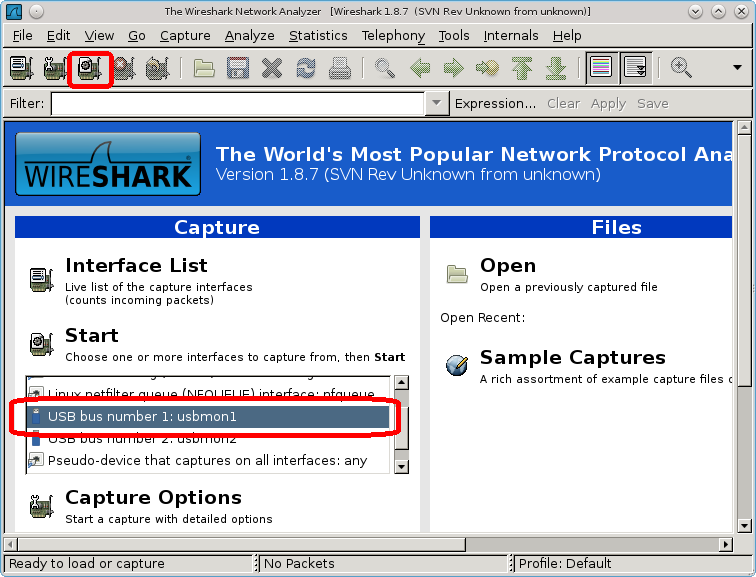
\includegraphics[width=10cm]{12_wireshark.png}
\end{figure}

Для анализа протокола нам необходимо перехватить следующие части генерируемого траффика:

\begin{itemize}
  \item инициализация устройства
  \item начало выполнения какой"=либо функции
  \item окончание выполнения какой"=либо функции
  \item деинициализация устройства
\end{itemize}

Обычно данные части отделены по времени, т.к. инициировать выполнения функции устройством можно в произвольное время (например, подвинуть мышку, нажать кнопку на клавиатуре, начать захват видео с веб"=камеры и т.д.)

Как правило, изучаемые устройства делятся на два типа:

\begin{itemize}
  \item Register"=oriented устройства
  \item Message"=oriented устройства
\end{itemize}

Для первых в перехватываемых трансферах будет чётко прослеживаться следующая структура:

\begin{itemize}
  \item заголовок трансфера (например, размер в байтах)
  \item адрес регистра
  \item значение (несколько значений)
  \item хвост трансфера (например, контрольная сумма)
\end{itemize}

Данные устройства предоставляют некое адресное пространство, в которое мы можем производить запись/чтение с помощью определённых USB"=трансферов.

Пример данного трансфера мы видим на иллюстрации:

\begin{figure}[h!]
  \centering
  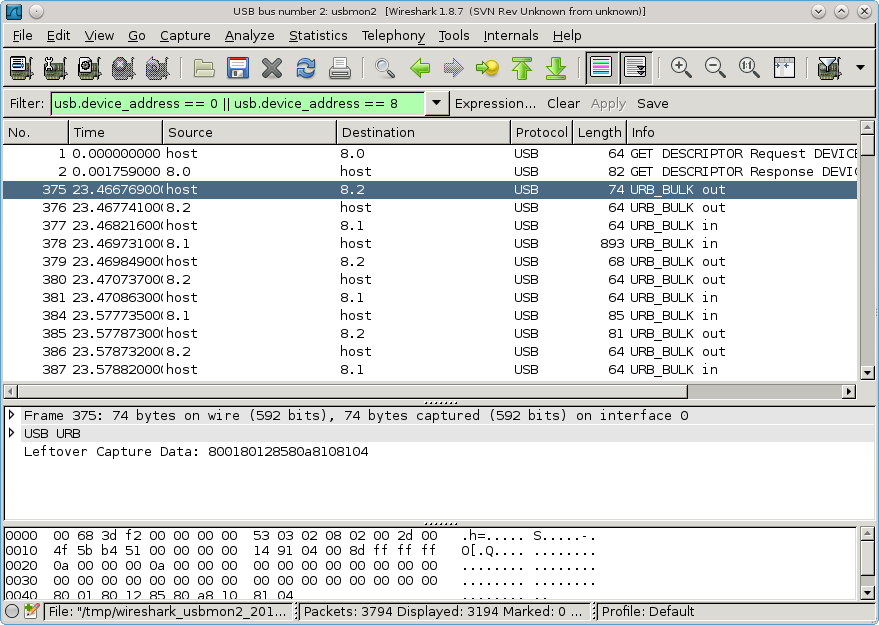
\includegraphics[width=10cm]{12_traffic-sample.png}
\end{figure}

См. трансфер \No 375, поле leftover capture data. В данном случае трансфер содержит пары адрес"=регистра "--- значение. Трансфер №376 является подтверждением, что устройство приняло трансфер. Трансфер \No 377 является запросом от хоста на приём данных от устройства, трансфер №378 "--- ответом устройства. Можно заметить, что любой трансфер в Wireshark виден как пара пакетов вида запрос хоста "--- ответ устройства (надеюсь, читатель еще помнить что все трансферы на USB шине инициирует хост?). Стоит отметить, что не всегда эта пара расположена линейно.

Для второго типа устройств в перехватываемых трансферах будет видна следующая структура:

\begin{itemize}
  \item заголовок трансфера
  \item тип сообщения
  \item тело сообщения
  \item хвост трансфера
\end{itemize}

Данные устройства, как правило, требуют больших усилий по расшифровке протокола.

Как правило, практически невозможно по дампу траффика, без экспериментов с устройством, расшифровать протокол. Для экспериментов удобно будет написать прототип драйвера с использованием библиотеки libusb. Данная библиотека работает в пространстве пользователя, т.о. при падении прототипа не упадёт вся ОС.

В качестве первого прототипа разумно будет повторить ту последовательность, которая записана в дампе. При запуске прототипа стоит записать еще один дамп, и сравнить его с оригинальным. Отличия между дампами сигнализируют о том, что что"=то прототип делает не так. Модификациями прототипа необходимо добиться идентичности дампа (в некоторых случаях это необязательно или невозможно, например при захвате картинки с камеры).

Пример простейших прототипов можно посмотреть в \cite{Anar4} и \cite{Anar5}. Как видно, эти прототипы состоят из следующих частей:

\begin{itemize}
  \item инициализация библиотеки: libusb\_init()
  \item открытие устройства: libusb\_open\_device\_with\_vid\_pid()
  \item выбор нужного интерфейса:  libusb\_claim\_interface()
  \item некоторого количества трансферов: libusb\_bulk\_transfer()/ \linebreak libusb\_control\_transfer()/libusb\_interrupt\_transfer()
  \item разбор ответа от устройства
  \item деинициализация: libusb\_close(); libusb\_exit()
\end{itemize}

\subsection*{Заключение}

Не смотря на то, что разбор протокола USB"=устройства кажется сложной задачей, на самом деле таковым не является "--- необходимо лишь упорство, терпение и желание экспериментировать.

\begin{thebibliography}{9}
\bibitem{Anar1} \url{http://www.beyondlogic.org/usbnutshell/usb1.shtml}
\bibitem{Anar2} \url{https://www.kernel.org/doc/Documentation/usb/usbmon.txt}
\bibitem{Anar3} \url{http://desowin.org/usbpcap/}
\bibitem{Anar4} \url{https://github.com/anarsoul/fprint\_aes1660}
\bibitem{Anar5} \url{https://github.com/anarsoul/fprint\_aes2550}
\end{thebibliography}

\end{document}





%\chapter{LVEE Winter 2012}
%\documentclass[10pt, a5paper]{article}
\usepackage{pdfpages}
\usepackage{parallel}
\usepackage[T2A]{fontenc}
\usepackage{ucs}
\usepackage[utf8x]{inputenc}
\usepackage[polish,english,russian]{babel}
\usepackage{hyperref}
\usepackage{rotating}
\usepackage[inner=2cm,top=1.8cm,outer=2cm,bottom=2.3cm,nohead]{geometry}
\usepackage{listings}
\usepackage{graphicx}
\usepackage{wrapfig}
\usepackage{longtable}
\usepackage{indentfirst}
\usepackage{array}
\newcolumntype{P}[1]{>{\raggedright\arraybackslash}p{#1}}
\frenchspacing
\usepackage{fixltx2e} %text sub- and superscripts
\usepackage{icomma} % коскі ў матэматычным рэжыме
\PreloadUnicodePage{4}

\newcommand{\longpage}{\enlargethispage{\baselineskip}}
\newcommand{\shortpage}{\enlargethispage{-\baselineskip}}

\def\switchlang#1{\expandafter\csname switchlang#1\endcsname}
\def\switchlangbe{
\let\saverefname=\refname%
\def\refname{Літаратура}%
\def\figurename{Іл.}%
}
\def\switchlangen{
\let\saverefname=\refname%
\def\refname{References}%
\def\figurename{Fig.}%
}
\def\switchlangru{
\let\saverefname=\refname%
\let\savefigurename=\figurename%
\def\refname{Литература}%
\def\figurename{Рис.}%
}

\hyphenation{admi-ni-stra-tive}
\hyphenation{ex-pe-ri-ence}
\hyphenation{fle-xi-bi-li-ty}
\hyphenation{Py-thon}
\hyphenation{ma-the-ma-ti-cal}
\hyphenation{re-ported}
\hyphenation{imp-le-menta-tions}
\hyphenation{pro-vides}
\hyphenation{en-gi-neering}
\hyphenation{com-pa-ti-bi-li-ty}
\hyphenation{im-pos-sible}
\hyphenation{desk-top}
\hyphenation{elec-tro-nic}
\hyphenation{com-pa-ny}
\hyphenation{de-ve-lop-ment}
\hyphenation{de-ve-loping}
\hyphenation{de-ve-lop}
\hyphenation{da-ta-ba-se}
\hyphenation{plat-forms}
\hyphenation{or-ga-ni-za-tion}
\hyphenation{pro-gramming}
\hyphenation{in-stru-ments}
\hyphenation{Li-nux}
\hyphenation{sour-ce}
\hyphenation{en-vi-ron-ment}
\hyphenation{Te-le-pathy}
\hyphenation{Li-nux-ov-ka}
\hyphenation{Open-BSD}
\hyphenation{Free-BSD}
\hyphenation{men-ti-on-ed}
\hyphenation{app-li-ca-tion}

\def\progref!#1!{\texttt{#1}}
\renewcommand{\arraystretch}{2} %Іначай формулы ў матрыцы зліпаюцца з лініямі
\usepackage{array}

\def\interview #1 (#2), #3, #4, #5\par{

\section[#1, #3, #4]{#1 -- #3, #4}
\def\qname{LVEE}
\def\aname{#1}
\def\q ##1\par{{\noindent \bf \qname: ##1 }\par}
\def\a{{\noindent \bf \aname: } \def\qname{L}\def\aname{#2}}
}

\def\interview* #1 (#2), #3, #4, #5\par{

\section*{#1\\{\small\rm #3, #4. #5}}

\def\qname{LVEE}
\def\aname{#1}
\def\q ##1\par{{\noindent \bf \qname: ##1 }\par}
\def\a{{\noindent \bf \aname: } \def\qname{L}\def\aname{#2}}
}


\begin{document}

\title{Software security}%\footnote{Текст данных и последующих тезисов, кроме специально оговоренных случаев, доступен под лицензией Creative Commons Attribution-ShareAlike 3.0}

\author{Алексей Чеусов\footnote{Минск, Беларусь}}
\maketitle

\begin{abstract}
System techniques and methods are reviewed for securing the software in UNIX World.
\end{abstract}

Язык программирования С, на десятилетия определивший успех операционных систем класса UNIX, на протяжении последних лет все чаще
становится источником проблем в области безопасности программного
обеспечения. Появившись как язык системного программирования, язык С
широко применяется также и для разработки прикладного ПО, что, ввиду принципиальной <<небезопасности>> этого языка, приводит к многочисленным проблемам, таким как получение доступа к системе злоумышленником, повышению привилегий процесса до уровня суперпользователя, rootkit-ам, нестабильности работы ОС и т.п. То же относится и к языку программирования С++.

В ближайшее время вряд ли стоит ожидать значительного падения популярности этих языков в области разработки как системного, так и прикладного ПО, поэтому
актуальной становится разработка средств и методов борьбы с
перечисленными выше проблемами менее радикальными, чем смена языка
программирования, средствами. Таким средствам и технологиям, существующим и развивающимся в различных UNIX"=подобных системах, посвящен настоящий краткий обзор.

К числу рассматриваемых технологий защиты можно среди прочих отнести следующие:

\begin{itemize}
  \item безопасные функции strl\{cat,cpy\} для работы со строками,
  \item SSP (stack smashing protection) "--- защита от переполнения стека,
  \item ASLR (address space layout randomization) "--- рандомизация базовых адресов сегментов виртуальной памяти процесса,
  \item PIE (position independent executable) "--- позиционно"=независимые исполняемые файлы,
  \item hardened chroot "--- усиленный chroot,
  \item W\^{}X "--- защита исполняемых сегментов памяти от записи и записываемых (стек и данные) от исполнения,
  \item PaX MPROTECT "--- защита mprotect(2),
  \item PaX Segvgard "--- защита от перебора адресов сегментов памяти приложения,
  \item Information filtering "--- сокрытие информации, доступной пользователям и процессам,
  \item per-user /tmp directory "--- размещение подкаталога временных файлов в домашней директории пользователя,
  \item SUID/SGIG executables "--- избавление от исполняемых файлов с установленным битом SUID,
  \item PAM tcb "--- замена PAM unix как средство избавления от бита SUID у passwd(8)
  \item capsicum "--- расширение POSIX API для обеспечения лучшей безопасности в системе UNIX.
  \item FUSE, PUFFS "--- подсистемы для реализации файловых систем в пространстве пользователя
  \item Микроядерные ОС "--- класс операционных систем, в которых основные сервисы работают на уровне пользователя, на уровне ядра же работает лишь самое необходимодое, за счет чего достигается надежность и безопасность
  \item RUMP "--- подсистема для запуска ядерного кода в пользовательском приложении
  \item SE Linux "--- подсистема контроля доступа в Linux
  \item kauth(9) "--- подсистема авторизации ядра NetBSD
  \item jail "--- система изоляции и виртуализации FreeBSD
\end{itemize}


\end{document}





%\documentclass[10pt, a5paper]{article}
\usepackage{pdfpages}
\usepackage{parallel}
\usepackage[T2A]{fontenc}
\usepackage{ucs}
\usepackage[utf8x]{inputenc}
\usepackage[polish,english,russian]{babel}
\usepackage{hyperref}
\usepackage{rotating}
\usepackage[inner=2cm,top=1.8cm,outer=2cm,bottom=2.3cm,nohead]{geometry}
\usepackage{listings}
\usepackage{graphicx}
\usepackage{wrapfig}
\usepackage{longtable}
\usepackage{indentfirst}
\usepackage{array}
\newcolumntype{P}[1]{>{\raggedright\arraybackslash}p{#1}}
\frenchspacing
\usepackage{fixltx2e} %text sub- and superscripts
\usepackage{icomma} % коскі ў матэматычным рэжыме
\PreloadUnicodePage{4}

\newcommand{\longpage}{\enlargethispage{\baselineskip}}
\newcommand{\shortpage}{\enlargethispage{-\baselineskip}}

\def\switchlang#1{\expandafter\csname switchlang#1\endcsname}
\def\switchlangbe{
\let\saverefname=\refname%
\def\refname{Літаратура}%
\def\figurename{Іл.}%
}
\def\switchlangen{
\let\saverefname=\refname%
\def\refname{References}%
\def\figurename{Fig.}%
}
\def\switchlangru{
\let\saverefname=\refname%
\let\savefigurename=\figurename%
\def\refname{Литература}%
\def\figurename{Рис.}%
}

\hyphenation{admi-ni-stra-tive}
\hyphenation{ex-pe-ri-ence}
\hyphenation{fle-xi-bi-li-ty}
\hyphenation{Py-thon}
\hyphenation{ma-the-ma-ti-cal}
\hyphenation{re-ported}
\hyphenation{imp-le-menta-tions}
\hyphenation{pro-vides}
\hyphenation{en-gi-neering}
\hyphenation{com-pa-ti-bi-li-ty}
\hyphenation{im-pos-sible}
\hyphenation{desk-top}
\hyphenation{elec-tro-nic}
\hyphenation{com-pa-ny}
\hyphenation{de-ve-lop-ment}
\hyphenation{de-ve-loping}
\hyphenation{de-ve-lop}
\hyphenation{da-ta-ba-se}
\hyphenation{plat-forms}
\hyphenation{or-ga-ni-za-tion}
\hyphenation{pro-gramming}
\hyphenation{in-stru-ments}
\hyphenation{Li-nux}
\hyphenation{sour-ce}
\hyphenation{en-vi-ron-ment}
\hyphenation{Te-le-pathy}
\hyphenation{Li-nux-ov-ka}
\hyphenation{Open-BSD}
\hyphenation{Free-BSD}
\hyphenation{men-ti-on-ed}
\hyphenation{app-li-ca-tion}

\def\progref!#1!{\texttt{#1}}
\renewcommand{\arraystretch}{2} %Іначай формулы ў матрыцы зліпаюцца з лініямі
\usepackage{array}

\def\interview #1 (#2), #3, #4, #5\par{

\section[#1, #3, #4]{#1 -- #3, #4}
\def\qname{LVEE}
\def\aname{#1}
\def\q ##1\par{{\noindent \bf \qname: ##1 }\par}
\def\a{{\noindent \bf \aname: } \def\qname{L}\def\aname{#2}}
}

\def\interview* #1 (#2), #3, #4, #5\par{

\section*{#1\\{\small\rm #3, #4. #5}}

\def\qname{LVEE}
\def\aname{#1}
\def\q ##1\par{{\noindent \bf \qname: ##1 }\par}
\def\a{{\noindent \bf \aname: } \def\qname{L}\def\aname{#2}}
}

\begin{document}
\title{Протокол IF-MAP}
\author{Олег Орел\footnote{Минск, Беларусь, EPAM Systems, \url{Aleh_Arol@epam.com}}}
\date{}
\maketitle
\begin{abstract}
The Interface for Metadata Access Points (IF-MAP) is an open standard client/server protocol developed as one of the core protocols of the Trusted Network Connect (TNC) open architec\-ture. IF-MAP provides a common interface between the database server acting as a clearinghouse for information about security events and objects, and other elements of the TNC architecture.
\end{abstract}

TNC (Trusted Network Connect) "--- архитектура, описывающая возможную реализацию подхода к сетевой компьютерной безопасности, унифицирующего решения по обеспечению безопасности на конечных узлах (такие как антивирусное ПО, системы обнаружения вторжений и т.~д.), пользовательскую аутентификацию, элементы обеспечения безопасности. Компьютер, подключившийся в сеть, получает уровень доступа к ресурсам по результатам анализа таких его параметров, как уровень защищенности от вредоносных программ, конфигурации, роли пользователя, обновлений ОС. По любому параметру доступ может быть разграничен: например, пользователь, чей компьютер не обладает свежими антивирусными базами, не будет допущен в Интернет. IF"=MAP "--- открытый стандарт, описывающий клиент"=серверный протокол обмена данных между элементами (MAP) в TNC"=архитектуре.
IF-MAP сервер "--- это централизованное хранилище метаданных (например, о состоянии узлов сети, пользователях и т.~д.), предоставляющее механизмы для публикации данных, поиска и подписок всем заинтересованным MAP"=клиентам. Модель данных, предусмотренная для IF-MAP сервиса, представляет собой граф, вершины которого "--- идентификаторы (device, ip-address, mac-address, access-request, \ldots), а ребра "--- метаданные. Например, метаданные типа ip-mac, которые публикует MAP"=клиент, работающий совместно с DHCP сервером, соединяют идентификаторы типа ip"=address и mac"=address (DHCP lease) и содержат дополнительную информацию (время действия адреса). MAP"=клиентам доступен поиск на этом графе, а система подписок на изменения позволяет выполнять отложенный поиск.


\end{document}



\documentclass[10pt, a5paper]{article}
\usepackage{pdfpages}
\usepackage{parallel}
\usepackage[T2A]{fontenc}
\usepackage{ucs}
\usepackage[utf8x]{inputenc}
\usepackage[polish,english,russian]{babel}
\usepackage{hyperref}
\usepackage{rotating}
\usepackage[inner=2cm,top=1.8cm,outer=2cm,bottom=2.3cm,nohead]{geometry}
\usepackage{listings}
\usepackage{graphicx}
\usepackage{wrapfig}
\usepackage{longtable}
\usepackage{indentfirst}
\usepackage{array}
\newcolumntype{P}[1]{>{\raggedright\arraybackslash}p{#1}}
\frenchspacing
\usepackage{fixltx2e} %text sub- and superscripts
\usepackage{icomma} % коскі ў матэматычным рэжыме
\PreloadUnicodePage{4}

\newcommand{\longpage}{\enlargethispage{\baselineskip}}
\newcommand{\shortpage}{\enlargethispage{-\baselineskip}}

\def\switchlang#1{\expandafter\csname switchlang#1\endcsname}
\def\switchlangbe{
\let\saverefname=\refname%
\def\refname{Літаратура}%
\def\figurename{Іл.}%
}
\def\switchlangen{
\let\saverefname=\refname%
\def\refname{References}%
\def\figurename{Fig.}%
}
\def\switchlangru{
\let\saverefname=\refname%
\let\savefigurename=\figurename%
\def\refname{Литература}%
\def\figurename{Рис.}%
}

\hyphenation{admi-ni-stra-tive}
\hyphenation{ex-pe-ri-ence}
\hyphenation{fle-xi-bi-li-ty}
\hyphenation{Py-thon}
\hyphenation{ma-the-ma-ti-cal}
\hyphenation{re-ported}
\hyphenation{imp-le-menta-tions}
\hyphenation{pro-vides}
\hyphenation{en-gi-neering}
\hyphenation{com-pa-ti-bi-li-ty}
\hyphenation{im-pos-sible}
\hyphenation{desk-top}
\hyphenation{elec-tro-nic}
\hyphenation{com-pa-ny}
\hyphenation{de-ve-lop-ment}
\hyphenation{de-ve-loping}
\hyphenation{de-ve-lop}
\hyphenation{da-ta-ba-se}
\hyphenation{plat-forms}
\hyphenation{or-ga-ni-za-tion}
\hyphenation{pro-gramming}
\hyphenation{in-stru-ments}
\hyphenation{Li-nux}
\hyphenation{sour-ce}
\hyphenation{en-vi-ron-ment}
\hyphenation{Te-le-pathy}
\hyphenation{Li-nux-ov-ka}
\hyphenation{Open-BSD}
\hyphenation{Free-BSD}
\hyphenation{men-ti-on-ed}
\hyphenation{app-li-ca-tion}

\def\progref!#1!{\texttt{#1}}
\renewcommand{\arraystretch}{2} %Іначай формулы ў матрыцы зліпаюцца з лініямі
\usepackage{array}

\def\interview #1 (#2), #3, #4, #5\par{

\section[#1, #3, #4]{#1 -- #3, #4}
\def\qname{LVEE}
\def\aname{#1}
\def\q ##1\par{{\noindent \bf \qname: ##1 }\par}
\def\a{{\noindent \bf \aname: } \def\qname{L}\def\aname{#2}}
}

\def\interview* #1 (#2), #3, #4, #5\par{

\section*{#1\\{\small\rm #3, #4. #5}}

\def\qname{LVEE}
\def\aname{#1}
\def\q ##1\par{{\noindent \bf \qname: ##1 }\par}
\def\a{{\noindent \bf \aname: } \def\qname{L}\def\aname{#2}}
}

\begin{document}
\title{Голос спонсора: SaM Solutions}
%\author{}
\date{}
\maketitle

Компания SaM Solutions выступает в роли системо-образующего спонсора конференции Linux Vacation Eastern Europe с момента рождения LVEE в 2005 году и на протяжении всех лет её проведения. 

Сложившаяся корпоративная практика не случайна. Продукты и решения, задействующие Linux и другие Free/Open Source Software проекты, составляют заметную часть пакета разработок SaM Solutions. Кадровая политика компании направлена на поощрение профессионального развития своих сотрудников, организацию их эффективного отдыха и привлечение хорошо мотивированных кандидатов к работе на компанию. Формат конференции LVEE успешно позволяет решать все три задачи. 

Одним из подразделений компании является отдел Linux и \linebreak Embbeded. Специалисты компании на протяжении десятилетий работают с СПО. Компанией реализован ряд проектов по адаптации ОС GNU/Linux для работы в различных устройствах, построенных на таких платформах как ARM, PowerPC, x86, MIPS. В последние годы "--- на ведущие позиции выходит разработка управляющего ПО для серверов Enterprise-класса, от низкоуровнего BMC Firmware на основе Linux до высокоуровневых систем контроля виртуализации и графических интерфейсов управления, от прошивок устройств хранения данных до BSP интегрированных плат для разработчика. Надёжность, качество и широкая функциональность множества свободных проектов позволяет строить нам системы любого уровня и сложности, опираясь на высококачественные готовые компоненты.

В рамках направления Linux и Embedded успешно выполнены проекты для таких знаковых заказчиков, как  Novell/SUSE, Fujitsu Technology Solutions  и осуществляется партнёрство с компаниями IBM и Oracle/Sun в области Open Source решений.

Мы разрабатываем, модифицируем и адаптируем различное свободное программное обеспечение для наших заказчиков, но не забываем и о своих нуждах "--- наши сотрудники используют в своей работе существующие програмные продукты и вносят вклад в их развитие. Часть внутренней инфраструктуры, а именно интранет-сеть компании, тестовые стенды отдела контроля качества, рабочие места сотрудников профильных подразделений "--- также работает под управлением СПО (серверные и десктопные платформы GNU/Linux и FreeBSD). 

В минувшем году, в рамках реорганизации, был разработан долгосрочный план развития направления Linux и Embedded в SaM Solutions. В нём впервые были кодифицированы уже имеющиеся внутренние неофициальные практики по взаимодействию с commu"=nity-based проектами. В частности разработаны меры и правила по
\begin{itemize}
  \item возврата изменений в родительские проекты (upstreaming);
  \item вхождения в состав постоянных разработчиков активно используемых нами FOSS-компонентов;
  \item публикации сообщений об ошибках (bug reporting);
  \item участия и помощи в организации community events;
  \item стимуляции докладов и участия в технических конференциях.
\end{itemize}
И план немедленно начал претворяться в жизнь.

Силами отдела организовано внутреннее обучение сотрудников на регулярной
основе. Был прочтен и опубликован курс по TDD. По согласованию с автором
опубликован курс Debian/Ubuntu Packaging (видео, презентация и исходные
тексты презентации в \LaTeX).  Были организованы и проведены курсы по
обучению QA специалистов для направления Embeded Linux. Проведено
практическое занятие по основам виртуализации и эмуляции, организована
лекция по вопросу профилирования и оптимизации Ruby-кода, лекция о
High-availability кластерах и направлении развития технологии. Кроме того,
проводился семинар по Video4Linux2. Для создания и обучения кадрового
резерва на ближайшее будущее запланированы постоянно действующие внутренние
проекты в области Embedded Linux, результаты которых также запланированы к
публикации.

Визиты представительных делегаций на Embedded World 2012 и Linux Con Europe/Embedded LinuxCon Europe 2011 обогатили нас новыми идеями, куда можно
двигаться дальше и что сейчас актуально. А выступления на Software
Engineering Forum for Students, круглом столе по СПО в рамках TIBO-2012
и LVEE Winter 2012 позволили поделиться опытом с
заинтересованными сторонами.

В апреле состоялась Ганноверская промышленная ярмарка \linebreak (Hannover Messe
2013). Компания SaM Solutions была представлена отдельным стендом, на
котором демонстрировались наработки в области встроенного и системного ПО
на базе OS Linux. Идея «умного» дома вызвала неподдельный интерес у
посетителей стенда.

При поддержке SaM Solutions, с декабря 2011 года возобновились регулярные встречи Minsk Linux Users Groups, под названием <<Линуксовка в SaM Solutions>>. Техническое оснащение линуксовок и открытый формат встреч позволил им практически мгновенно стать заметным дискуссионным клубом по широкому спектру вопросов, прямо или косвенно связанных с СПО. Свободная картография (OpenStreetMap), технологии виртуализации, минский \linebreak hackerspace, Linux Mobile, бойкот Голливудской продукции, systemd, загрузчик u-boot, белорусская локализация GNOME --- это только часть тем, поднятых за последние линуксовки.

Быстрые и положительные изменения, как внутри компании SaM Solutions, так и в экосфере СПО (и Linux в частности) наполняют нас уверенностью, что направление движения выбрано верно.

\begin{figure}[h!]
\centering
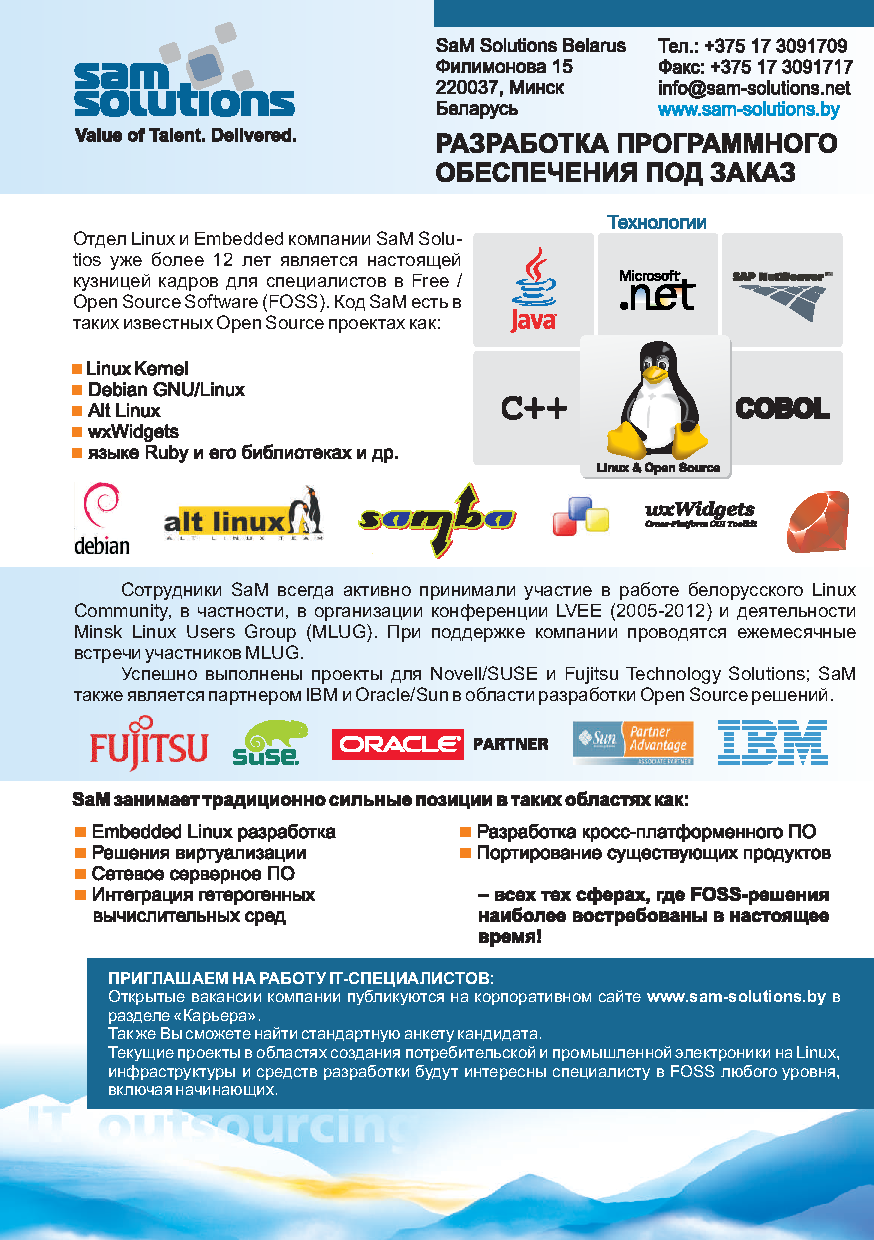
\includegraphics[height=11.8cm]{48_spons_sams.pdf}
\end{figure}
\end{document}



\documentclass[10pt, a5paper]{article}
\usepackage{pdfpages}
\usepackage{parallel}
\usepackage[T2A]{fontenc}
\usepackage{ucs}
\usepackage[utf8x]{inputenc}
\usepackage[polish,english,russian]{babel}
\usepackage{hyperref}
\usepackage{rotating}
\usepackage[inner=2cm,top=1.8cm,outer=2cm,bottom=2.3cm,nohead]{geometry}
\usepackage{listings}
\usepackage{graphicx}
\usepackage{wrapfig}
\usepackage{longtable}
\usepackage{indentfirst}
\usepackage{array}
\newcolumntype{P}[1]{>{\raggedright\arraybackslash}p{#1}}
\frenchspacing
\usepackage{fixltx2e} %text sub- and superscripts
\usepackage{icomma} % коскі ў матэматычным рэжыме
\PreloadUnicodePage{4}

\newcommand{\longpage}{\enlargethispage{\baselineskip}}
\newcommand{\shortpage}{\enlargethispage{-\baselineskip}}

\def\switchlang#1{\expandafter\csname switchlang#1\endcsname}
\def\switchlangbe{
\let\saverefname=\refname%
\def\refname{Літаратура}%
\def\figurename{Іл.}%
}
\def\switchlangen{
\let\saverefname=\refname%
\def\refname{References}%
\def\figurename{Fig.}%
}
\def\switchlangru{
\let\saverefname=\refname%
\let\savefigurename=\figurename%
\def\refname{Литература}%
\def\figurename{Рис.}%
}

\hyphenation{admi-ni-stra-tive}
\hyphenation{ex-pe-ri-ence}
\hyphenation{fle-xi-bi-li-ty}
\hyphenation{Py-thon}
\hyphenation{ma-the-ma-ti-cal}
\hyphenation{re-ported}
\hyphenation{imp-le-menta-tions}
\hyphenation{pro-vides}
\hyphenation{en-gi-neering}
\hyphenation{com-pa-ti-bi-li-ty}
\hyphenation{im-pos-sible}
\hyphenation{desk-top}
\hyphenation{elec-tro-nic}
\hyphenation{com-pa-ny}
\hyphenation{de-ve-lop-ment}
\hyphenation{de-ve-loping}
\hyphenation{de-ve-lop}
\hyphenation{da-ta-ba-se}
\hyphenation{plat-forms}
\hyphenation{or-ga-ni-za-tion}
\hyphenation{pro-gramming}
\hyphenation{in-stru-ments}
\hyphenation{Li-nux}
\hyphenation{sour-ce}
\hyphenation{en-vi-ron-ment}
\hyphenation{Te-le-pathy}
\hyphenation{Li-nux-ov-ka}
\hyphenation{Open-BSD}
\hyphenation{Free-BSD}
\hyphenation{men-ti-on-ed}
\hyphenation{app-li-ca-tion}

\def\progref!#1!{\texttt{#1}}
\renewcommand{\arraystretch}{2} %Іначай формулы ў матрыцы зліпаюцца з лініямі
\usepackage{array}

\def\interview #1 (#2), #3, #4, #5\par{

\section[#1, #3, #4]{#1 -- #3, #4}
\def\qname{LVEE}
\def\aname{#1}
\def\q ##1\par{{\noindent \bf \qname: ##1 }\par}
\def\a{{\noindent \bf \aname: } \def\qname{L}\def\aname{#2}}
}

\def\interview* #1 (#2), #3, #4, #5\par{

\section*{#1\\{\small\rm #3, #4. #5}}

\def\qname{LVEE}
\def\aname{#1}
\def\q ##1\par{{\noindent \bf \qname: ##1 }\par}
\def\a{{\noindent \bf \aname: } \def\qname{L}\def\aname{#2}}
}

\begin{document}
\title{Голос спонсора: EPAM Systems}
%\author{}
\date{}
\maketitle

Компания EPAM Systems не первый год является спонсором международной конференции разработчиков и пользователей свободного программного обеспечения LVEE (Linux Vacation / Eastern Europe). Этот год также не стал исключением. Пожалуй, LVEE является самым значимым событием для русскоязычных разработчиков и тестировщиков Open Source. Каждое лето здесь встречаются начинающие специалисты и «ветераны»"=разработчики из десятка стран для обмена опытом и общения на профессиональные темы. Наши специалисты также активно участвуют в данной конференции: в качестве докладчиков и организаторов/волонтёров. Это уникальная в своём роде конференция, и именно поэтому EPAM Systems очередной раз принимает участие в LVEE в качестве спонсора.


EPAM Systems "--- одна из крупнейших компаний"=поставщиков\linebreak услуг в области разработки программного обеспечения и решений на территории СНГ и Центральной и Восточной Европы. Созданная в 1993 году, сегодня она имеет представительства в 12 странах мира, в штате работают более 9 тыс. сотрудников, из которых более 3 тыс. "--- в Беларуси. Рост компании обеспечивается за счет собственных обучающих программ и передаче опыта от больших специалистов до начинающих разработчиков. Компания EPAM Systems выполняет проекты более чем в 30 странах мира. Основные направления деятельности: разработка, тестирование, сопровождение и поддержка заказного программного обеспечения и бизнес"=приложений, а также ИТ"=консалтинг с учетом отраслевой специфики бизнеса.

Наша компания участвует в проектах с такими крупными, хорошо известными заказчиками как Google, Novell, Infoblox, Parallels, 10Gen и др., так и с небольшими, в том числе и с начинающими свой путь в софтверном бизнесе.


К примеру, для Infoblox была реализована связка между WebUI с BIND и DHCP. Для этого был разработан комплекс решений под управлением Shell и Python скриптов, а также механизм позволяющий вносить правки в BIND и DHCP на языке C. Также был разработан развернутый функционал, автоматизирующий инсталляцию новых устройств и их эксплуатацию, что позволяет значительно упростить управление данными. Встроенный Web"=интерфейс позволяет разворачивать, управлять сервисами DNS, DNSSEC, DHCP, IPAM, устанавливать новые версии ПО, архивировать и восстанавливать из архивов необходимые данные, восстанавливать их после аварии, проводить мониторинг сети и создавать отчеты без необходимости обращения к командной строке.


Еще одним решением, реализованным для компании Infoblox, являлся программный продукт, позволяющий контролировать сетевые изменения, таким образом, облегчая идентификацию трудноуловимых проблем конфигурации и соответствие требованиям. Вместо того чтобы просто регистрировать изменения, система использует внесенную информацию для проверки, анализа и автоматической обработки сетевых изменений. Благодаря инновационной, квалифицированной, глубокой технике логического анализа, программа изолирует проблемы исправности и конфигурации до того, как они могут вызвать более серьезные сбои.


Разработанная для анализа сложных сетей система изучает сеть, собирает ключевую информацию, применяет встроенную технику логического анализа и создает оценку исправности сети и список проблем, требующих принятие мер для улучшения качества работы сети.


Правильное использование свободного ПО в разработках сокращает и расходы на покупку лицензионных программ, и трудозатраты при создании коммерческого ПО. Немалую роль для достижения превосходного результата играет привлечение к разработке опытных специалистов. LVEE способствует появлению таких специалистов, развитию их навыков и расширению кругозора. Хотелось бы пожелать участникам конференции интересных проектов и максимум пользы от участия в LVEE.


\end{document}



\documentclass[10pt, a5paper]{article}
\usepackage{pdfpages}
\usepackage{parallel}
\usepackage[T2A]{fontenc}
\usepackage{ucs}
\usepackage[utf8x]{inputenc}
\usepackage[polish,english,russian]{babel}
\usepackage{hyperref}
\usepackage{rotating}
\usepackage[inner=2cm,top=1.8cm,outer=2cm,bottom=2.3cm,nohead]{geometry}
\usepackage{listings}
\usepackage{graphicx}
\usepackage{wrapfig}
\usepackage{longtable}
\usepackage{indentfirst}
\usepackage{array}
\newcolumntype{P}[1]{>{\raggedright\arraybackslash}p{#1}}
\frenchspacing
\usepackage{fixltx2e} %text sub- and superscripts
\usepackage{icomma} % коскі ў матэматычным рэжыме
\PreloadUnicodePage{4}

\newcommand{\longpage}{\enlargethispage{\baselineskip}}
\newcommand{\shortpage}{\enlargethispage{-\baselineskip}}

\def\switchlang#1{\expandafter\csname switchlang#1\endcsname}
\def\switchlangbe{
\let\saverefname=\refname%
\def\refname{Літаратура}%
\def\figurename{Іл.}%
}
\def\switchlangen{
\let\saverefname=\refname%
\def\refname{References}%
\def\figurename{Fig.}%
}
\def\switchlangru{
\let\saverefname=\refname%
\let\savefigurename=\figurename%
\def\refname{Литература}%
\def\figurename{Рис.}%
}

\hyphenation{admi-ni-stra-tive}
\hyphenation{ex-pe-ri-ence}
\hyphenation{fle-xi-bi-li-ty}
\hyphenation{Py-thon}
\hyphenation{ma-the-ma-ti-cal}
\hyphenation{re-ported}
\hyphenation{imp-le-menta-tions}
\hyphenation{pro-vides}
\hyphenation{en-gi-neering}
\hyphenation{com-pa-ti-bi-li-ty}
\hyphenation{im-pos-sible}
\hyphenation{desk-top}
\hyphenation{elec-tro-nic}
\hyphenation{com-pa-ny}
\hyphenation{de-ve-lop-ment}
\hyphenation{de-ve-loping}
\hyphenation{de-ve-lop}
\hyphenation{da-ta-ba-se}
\hyphenation{plat-forms}
\hyphenation{or-ga-ni-za-tion}
\hyphenation{pro-gramming}
\hyphenation{in-stru-ments}
\hyphenation{Li-nux}
\hyphenation{sour-ce}
\hyphenation{en-vi-ron-ment}
\hyphenation{Te-le-pathy}
\hyphenation{Li-nux-ov-ka}
\hyphenation{Open-BSD}
\hyphenation{Free-BSD}
\hyphenation{men-ti-on-ed}
\hyphenation{app-li-ca-tion}

\def\progref!#1!{\texttt{#1}}
\renewcommand{\arraystretch}{2} %Іначай формулы ў матрыцы зліпаюцца з лініямі
\usepackage{array}

\def\interview #1 (#2), #3, #4, #5\par{

\section[#1, #3, #4]{#1 -- #3, #4}
\def\qname{LVEE}
\def\aname{#1}
\def\q ##1\par{{\noindent \bf \qname: ##1 }\par}
\def\a{{\noindent \bf \aname: } \def\qname{L}\def\aname{#2}}
}

\def\interview* #1 (#2), #3, #4, #5\par{

\section*{#1\\{\small\rm #3, #4. #5}}

\def\qname{LVEE}
\def\aname{#1}
\def\q ##1\par{{\noindent \bf \qname: ##1 }\par}
\def\a{{\noindent \bf \aname: } \def\qname{L}\def\aname{#2}}
}

%\frenchspacing
\begin{document}
\title{Голос спонсора: ITS Partner}
%\author{}
\date{}
\maketitle%

~

\end{document}



\documentclass[10pt, a5paper]{article}
\usepackage{pdfpages}
\usepackage{parallel}
\usepackage[T2A]{fontenc}
\usepackage{ucs}
\usepackage[utf8x]{inputenc}
\usepackage[polish,english,russian]{babel}
\usepackage{hyperref}
\usepackage{rotating}
\usepackage[inner=2cm,top=1.8cm,outer=2cm,bottom=2.3cm,nohead]{geometry}
\usepackage{listings}
\usepackage{graphicx}
\usepackage{wrapfig}
\usepackage{longtable}
\usepackage{indentfirst}
\usepackage{array}
\newcolumntype{P}[1]{>{\raggedright\arraybackslash}p{#1}}
\frenchspacing
\usepackage{fixltx2e} %text sub- and superscripts
\usepackage{icomma} % коскі ў матэматычным рэжыме
\PreloadUnicodePage{4}

\newcommand{\longpage}{\enlargethispage{\baselineskip}}
\newcommand{\shortpage}{\enlargethispage{-\baselineskip}}

\def\switchlang#1{\expandafter\csname switchlang#1\endcsname}
\def\switchlangbe{
\let\saverefname=\refname%
\def\refname{Літаратура}%
\def\figurename{Іл.}%
}
\def\switchlangen{
\let\saverefname=\refname%
\def\refname{References}%
\def\figurename{Fig.}%
}
\def\switchlangru{
\let\saverefname=\refname%
\let\savefigurename=\figurename%
\def\refname{Литература}%
\def\figurename{Рис.}%
}

\hyphenation{admi-ni-stra-tive}
\hyphenation{ex-pe-ri-ence}
\hyphenation{fle-xi-bi-li-ty}
\hyphenation{Py-thon}
\hyphenation{ma-the-ma-ti-cal}
\hyphenation{re-ported}
\hyphenation{imp-le-menta-tions}
\hyphenation{pro-vides}
\hyphenation{en-gi-neering}
\hyphenation{com-pa-ti-bi-li-ty}
\hyphenation{im-pos-sible}
\hyphenation{desk-top}
\hyphenation{elec-tro-nic}
\hyphenation{com-pa-ny}
\hyphenation{de-ve-lop-ment}
\hyphenation{de-ve-loping}
\hyphenation{de-ve-lop}
\hyphenation{da-ta-ba-se}
\hyphenation{plat-forms}
\hyphenation{or-ga-ni-za-tion}
\hyphenation{pro-gramming}
\hyphenation{in-stru-ments}
\hyphenation{Li-nux}
\hyphenation{sour-ce}
\hyphenation{en-vi-ron-ment}
\hyphenation{Te-le-pathy}
\hyphenation{Li-nux-ov-ka}
\hyphenation{Open-BSD}
\hyphenation{Free-BSD}
\hyphenation{men-ti-on-ed}
\hyphenation{app-li-ca-tion}

\def\progref!#1!{\texttt{#1}}
\renewcommand{\arraystretch}{2} %Іначай формулы ў матрыцы зліпаюцца з лініямі
\usepackage{array}

\def\interview #1 (#2), #3, #4, #5\par{

\section[#1, #3, #4]{#1 -- #3, #4}
\def\qname{LVEE}
\def\aname{#1}
\def\q ##1\par{{\noindent \bf \qname: ##1 }\par}
\def\a{{\noindent \bf \aname: } \def\qname{L}\def\aname{#2}}
}

\def\interview* #1 (#2), #3, #4, #5\par{

\section*{#1\\{\small\rm #3, #4. #5}}

\def\qname{LVEE}
\def\aname{#1}
\def\q ##1\par{{\noindent \bf \qname: ##1 }\par}
\def\a{{\noindent \bf \aname: } \def\qname{L}\def\aname{#2}}
}

\begin{document}
\title{Голос спонсора: World of Tanks team}
%\author{}
\date{}
\maketitle

\subsection*{О проекте}

World of Tanks (Мир танков) "--- первый ММО проект ААА класса, созданный
белоруской командой. Разработчиками игра позиционируется как MMO"=экшн с
элементами ролевой игры, шутера и стратегии. Концепция <<World of Tanks>>
базируется на массовых командных танковых сражениях в режиме PvP. Онлайн
релиз русской версии игры состоялся 12 августа 2010 года, в марте 2011 года
состоялся <<китайский>> релиз, а в апреле 2011 года проект успешно вышел на
территории США и Европы.

Успех проекта World of Tanks можно оценить по целому ряду показателей:
количество активных игроков более 2 миллионов, рекордная цифра одновременной
игры "--- более 150.000 игроков на российском игровом кластере! В книгу
рекордов Гиннеса мы вошли 23 января 2011 года с показателем 91 311 игроков
он"=лайн. 

Дважды подряд в 2010 и 2011 году на Конференции Разработчиков Компьютерных
Игр (Москва) наш проект был признан Лучшей клиентской он"=лайн игрой (КРИ
2010) и Лучшей игрой (КРИ 2011).

В 2010 году по результатам международной выставки E3 (Лос"=Анжелес)
крупнейший ММО"=портал Massivly назвал наш проект New Concept 2010. В
настоящий момент определяются победители E3 2011. Мы сможем рассказать о
наших успехах уже при личной встрече на конференции LVEE 2011.

\subsection*{Подробности о проекте}

Игровые кластеры проекта находятся в дата"=центрах России, Германии, США и
Китая. Общее количество серверов в настоящий момент порядка 500, к концу
года мы планируем удвоить их количество.

Как игровые, так и прочие инфраструктурные сервера функционируют на базе
операционной системы CentOS.

Осенью 2010 года пики онлайна на российском игровом кластере достигали 30
тыс. В настоящий момент за счет высокотехнологичных решений наших
специалистов (включающих в себя оптимизацию сетевой инфраструктуры,
оптимизацию работы с базами данных, оптимизацию нашего серверного ПО) пик
он-лайна вырос до 150 тыс.

Высокая производительность достигается в т.~ч. за счет использования
free and open source software  как технологической основы для работы
серверной части самой масштабной ММО"=игры, а именно: CentOS,
MySQL, nginx, zabbix, nagios, cacti, python, django и т.~д.

\subsection*{О нас}

Над созданием проекта работает СООО <<Гейм Стрим>> "--- основной центр разработки
компании \url{Wargaming.net}. История компании "--- это 12"=летний опыт создания игр,
более 15 выпущенных проектов, среди которых <<Операция Багратион>>, а так же
<<Order of War>>, изданная Square Enix. В 2007 году мы объединились с минской
студией Arise. В 2010 из разработчика превратились в издателя "--- мы сами
осуществляем оперирование проекта World of Tanks. 

Наши награды на Конференции Разработчиков Компьютерных Игр (Москва): лучшая стратегическая игра КРИ"=2008 (проект <<Операция Багратион>>),
приз от прессы КРИ"=2009, лучшая компания"=разработчик КРИ"=2009 и КРИ"=2010, приз от индустрии КРИ 2011, приз зрительских симпатий КРИ 2011.

Сейчас в студии работает более 200 человек. Мы готовимся к запуску в
производство новых проектов и будем рады знакомству с талантливыми
специалистами. 

Нашим будущим сотрудникам мы предлагаем уникальную возможность работать над
онлайн"=проектами ААА класса, с применением передовых технологических
решений; реализовать себя, работая над сложными задачами; учиться у ведущих
специалистов отрасли. Со своей стороны мы создаём для этого все условия:
комфортный офис, современное техническое обеспечение рабочих мест, все
социальные гарантии, высокие белые зарплаты, обучение и т.~д. А ещё у нас
работают замечательные люди.

Наш контактный e-mail:  \url{rabota@wargaming.net}
Присоединяйтесь к команде World of Tanks!

\end{document}



\documentclass[10pt, a5paper]{article}
\usepackage{pdfpages}
\usepackage{parallel}
\usepackage[T2A]{fontenc}
\usepackage{ucs}
\usepackage[utf8x]{inputenc}
\usepackage[polish,english,russian]{babel}
\usepackage{hyperref}
\usepackage{rotating}
\usepackage[inner=2cm,top=1.8cm,outer=2cm,bottom=2.3cm,nohead]{geometry}
\usepackage{listings}
\usepackage{graphicx}
\usepackage{wrapfig}
\usepackage{longtable}
\usepackage{indentfirst}
\usepackage{array}
\newcolumntype{P}[1]{>{\raggedright\arraybackslash}p{#1}}
\frenchspacing
\usepackage{fixltx2e} %text sub- and superscripts
\usepackage{icomma} % коскі ў матэматычным рэжыме
\PreloadUnicodePage{4}

\newcommand{\longpage}{\enlargethispage{\baselineskip}}
\newcommand{\shortpage}{\enlargethispage{-\baselineskip}}

\def\switchlang#1{\expandafter\csname switchlang#1\endcsname}
\def\switchlangbe{
\let\saverefname=\refname%
\def\refname{Літаратура}%
\def\figurename{Іл.}%
}
\def\switchlangen{
\let\saverefname=\refname%
\def\refname{References}%
\def\figurename{Fig.}%
}
\def\switchlangru{
\let\saverefname=\refname%
\let\savefigurename=\figurename%
\def\refname{Литература}%
\def\figurename{Рис.}%
}

\hyphenation{admi-ni-stra-tive}
\hyphenation{ex-pe-ri-ence}
\hyphenation{fle-xi-bi-li-ty}
\hyphenation{Py-thon}
\hyphenation{ma-the-ma-ti-cal}
\hyphenation{re-ported}
\hyphenation{imp-le-menta-tions}
\hyphenation{pro-vides}
\hyphenation{en-gi-neering}
\hyphenation{com-pa-ti-bi-li-ty}
\hyphenation{im-pos-sible}
\hyphenation{desk-top}
\hyphenation{elec-tro-nic}
\hyphenation{com-pa-ny}
\hyphenation{de-ve-lop-ment}
\hyphenation{de-ve-loping}
\hyphenation{de-ve-lop}
\hyphenation{da-ta-ba-se}
\hyphenation{plat-forms}
\hyphenation{or-ga-ni-za-tion}
\hyphenation{pro-gramming}
\hyphenation{in-stru-ments}
\hyphenation{Li-nux}
\hyphenation{sour-ce}
\hyphenation{en-vi-ron-ment}
\hyphenation{Te-le-pathy}
\hyphenation{Li-nux-ov-ka}
\hyphenation{Open-BSD}
\hyphenation{Free-BSD}
\hyphenation{men-ti-on-ed}
\hyphenation{app-li-ca-tion}

\def\progref!#1!{\texttt{#1}}
\renewcommand{\arraystretch}{2} %Іначай формулы ў матрыцы зліпаюцца з лініямі
\usepackage{array}

\def\interview #1 (#2), #3, #4, #5\par{

\section[#1, #3, #4]{#1 -- #3, #4}
\def\qname{LVEE}
\def\aname{#1}
\def\q ##1\par{{\noindent \bf \qname: ##1 }\par}
\def\a{{\noindent \bf \aname: } \def\qname{L}\def\aname{#2}}
}

\def\interview* #1 (#2), #3, #4, #5\par{

\section*{#1\\{\small\rm #3, #4. #5}}

\def\qname{LVEE}
\def\aname{#1}
\def\q ##1\par{{\noindent \bf \qname: ##1 }\par}
\def\a{{\noindent \bf \aname: } \def\qname{L}\def\aname{#2}}
}

\begin{document}
\title{Голос спонсора: Promwad}
%\author{}
\date{}
\maketitle
%\begin{wrapfigure}{l}{0.3\textwidth}

\begin{figure}[h!]
\centering

\includegraphics[width=10cm]{53_spons_promwad.png}
\end{figure}

{\bf Инновационная компания Promwad} реализует полный цикл разработки электроники: создание концепции продукта, промышленный дизайн и конструирование, проектирование аппаратных \linebreak платформ, разработка встроенного и прикладного ПО, тестирование ПО и контроль качества, сертификация, изготовление опытных образцов, постановка и сопровождение массового производства.

Promwad предлагает услуги аутсорсинга разработки электронных устройств в различных отраслях рынка электроники: телекоммуникации, автомобильная электроника, автоматизация, потребительская электроника, медиа и развлечения и другие. 

Разработка встроенного ПО "--- одна из основных услуг и направлений развития Promwad. Мы разрабатываем ПО для микропроцессоров, систем-на-кристалле, цифровых сигнальных процессоров и микроконтроллеров.

Наши разработчики работают с:
\begin{itemize}
\item Операционными системами "--- GNU/Linux, Android, FreeRTOS, RTEMS и другие специализированные RTOS
\item Языками программирования "--- C (user-space, kernel-space),\linebreak ARM Assembler, C++, Unix shell, Lua, Python, Javascript
\item Графическими библиотеками "--- QT+QML, SDL, OpenGL
\item Linux подсистемами "--- network drivers, USB, PCI, UART, SPI, I2C, GPIO, IRQs, Real time scheduling, cryptography, DMA, PMIC, ALSA, touchscreen, sensors, framebuffer, v4l2
\item Базами данных "--- MySQL, sqlite
\item Средствами сборки "--- make, Automake/Autotools, Cmake, \linebreak Qmak
\item Сборочными системами, фреймворками "--- Buildroot, \linebreak OpenEmbedded, Yocto, Openwrt, rpm/rpmbuild, deb/debuild, uClinux, STAPI
\item Отладками "--- jtag, openocd, valgrind, gdb
\item Системами контроля версий "--- SVN, GIT
\end{itemize}

В компании всегда открыт набор специалистов- разработчиков Linux Embedded, имеющих опыт работы  на языке программирования С/С++  в сфере Embedded не менее двух лет.

Сегодня Promwad "--- это успешная компания на рынке электроники и IT, резидент Парка высоких технологий (ПВТ), участник партнерских программ ведущих мировых производителей электронных компонентов, таких как Texas Instruments, STMicroelectronics, Analog Devices, Marvell и Fujitsu. 

Как современная компания мы уделяем внимание внутренним ценностям: обучение, развитие сотрудников, активный отдых, спонсорство и участие в тематических конференциях и тп. (с 2007 года Promwad постоянный спонсор конференций LVEE, а с 2009 года проводит собственный Форум разработчиков цифровой электроники "--- DEDF).

Как социально ответственная компания мы являемся партнером и титульным спонсором Кубка приключенческих гонок "--- ПромвадТур, который объединяет неравнодушных к активному досугу и приключениям единомышленников различных профессий. 

Описание услуг  компании, портфолио выполненных проектов, текущие вакансии и другую полезную информацию смотрите на корпоративном сайте Promwad: \url{www.promwad.com}.

{\bf Мы любим то, что делаем, и работаем на результат! Если ты разделяешь нашу позицию "--- будем рады принять в команду!}

%\documentclass[10pt, a5paper]{article}
\usepackage{pdfpages}
\usepackage{parallel}
\usepackage[T2A]{fontenc}
\usepackage{ucs}
\usepackage[utf8x]{inputenc}
\usepackage[polish,english,russian]{babel}
\usepackage{hyperref}
\usepackage{rotating}
\usepackage[inner=2cm,top=1.8cm,outer=2cm,bottom=2.3cm,nohead]{geometry}
\usepackage{listings}
\usepackage{graphicx}
\usepackage{wrapfig}
\usepackage{longtable}
\usepackage{indentfirst}
\usepackage{array}
\newcolumntype{P}[1]{>{\raggedright\arraybackslash}p{#1}}
\frenchspacing
\usepackage{fixltx2e} %text sub- and superscripts
\usepackage{icomma} % коскі ў матэматычным рэжыме
\PreloadUnicodePage{4}

\newcommand{\longpage}{\enlargethispage{\baselineskip}}
\newcommand{\shortpage}{\enlargethispage{-\baselineskip}}

\def\switchlang#1{\expandafter\csname switchlang#1\endcsname}
\def\switchlangbe{
\let\saverefname=\refname%
\def\refname{Літаратура}%
\def\figurename{Іл.}%
}
\def\switchlangen{
\let\saverefname=\refname%
\def\refname{References}%
\def\figurename{Fig.}%
}
\def\switchlangru{
\let\saverefname=\refname%
\let\savefigurename=\figurename%
\def\refname{Литература}%
\def\figurename{Рис.}%
}

\hyphenation{admi-ni-stra-tive}
\hyphenation{ex-pe-ri-ence}
\hyphenation{fle-xi-bi-li-ty}
\hyphenation{Py-thon}
\hyphenation{ma-the-ma-ti-cal}
\hyphenation{re-ported}
\hyphenation{imp-le-menta-tions}
\hyphenation{pro-vides}
\hyphenation{en-gi-neering}
\hyphenation{com-pa-ti-bi-li-ty}
\hyphenation{im-pos-sible}
\hyphenation{desk-top}
\hyphenation{elec-tro-nic}
\hyphenation{com-pa-ny}
\hyphenation{de-ve-lop-ment}
\hyphenation{de-ve-loping}
\hyphenation{de-ve-lop}
\hyphenation{da-ta-ba-se}
\hyphenation{plat-forms}
\hyphenation{or-ga-ni-za-tion}
\hyphenation{pro-gramming}
\hyphenation{in-stru-ments}
\hyphenation{Li-nux}
\hyphenation{sour-ce}
\hyphenation{en-vi-ron-ment}
\hyphenation{Te-le-pathy}
\hyphenation{Li-nux-ov-ka}
\hyphenation{Open-BSD}
\hyphenation{Free-BSD}
\hyphenation{men-ti-on-ed}
\hyphenation{app-li-ca-tion}

\def\progref!#1!{\texttt{#1}}
\renewcommand{\arraystretch}{2} %Іначай формулы ў матрыцы зліпаюцца з лініямі
\usepackage{array}

\def\interview #1 (#2), #3, #4, #5\par{

\section[#1, #3, #4]{#1 -- #3, #4}
\def\qname{LVEE}
\def\aname{#1}
\def\q ##1\par{{\noindent \bf \qname: ##1 }\par}
\def\a{{\noindent \bf \aname: } \def\qname{L}\def\aname{#2}}
}

\def\interview* #1 (#2), #3, #4, #5\par{

\section*{#1\\{\small\rm #3, #4. #5}}

\def\qname{LVEE}
\def\aname{#1}
\def\q ##1\par{{\noindent \bf \qname: ##1 }\par}
\def\a{{\noindent \bf \aname: } \def\qname{L}\def\aname{#2}}
}

\begin{document}
\title{Голос спонсора: компания Анакреон}
%\author{}
\date{}
\maketitle
\begin{figure}[h!]
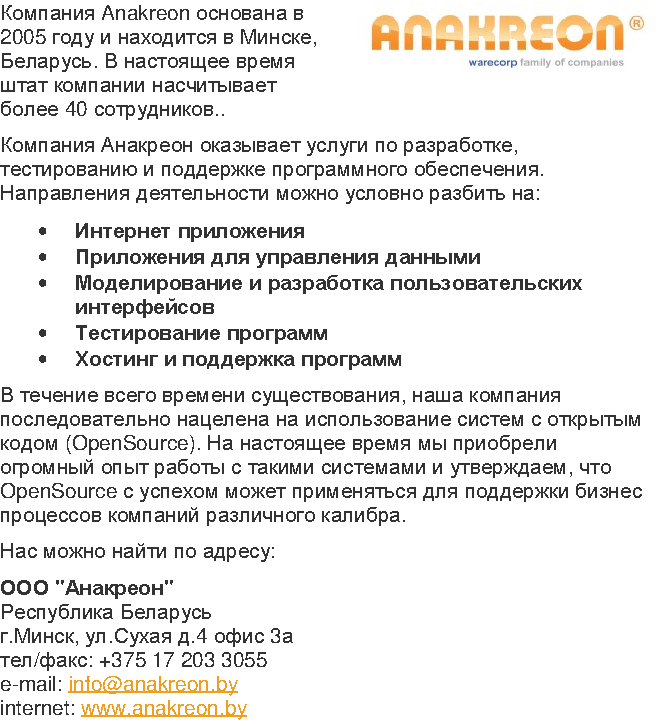
\includegraphics[width=11cm]{54_spons_anakreon.pdf}
\end{figure}
\end{document}



\documentclass[10pt, a5paper]{article}
\usepackage{pdfpages}
\usepackage{parallel}
\usepackage[T2A]{fontenc}
\usepackage{ucs}
\usepackage[utf8x]{inputenc}
\usepackage[polish,english,russian]{babel}
\usepackage{hyperref}
\usepackage{rotating}
\usepackage[inner=2cm,top=1.8cm,outer=2cm,bottom=2.3cm,nohead]{geometry}
\usepackage{listings}
\usepackage{graphicx}
\usepackage{wrapfig}
\usepackage{longtable}
\usepackage{indentfirst}
\usepackage{array}
\newcolumntype{P}[1]{>{\raggedright\arraybackslash}p{#1}}
\frenchspacing
\usepackage{fixltx2e} %text sub- and superscripts
\usepackage{icomma} % коскі ў матэматычным рэжыме
\PreloadUnicodePage{4}

\newcommand{\longpage}{\enlargethispage{\baselineskip}}
\newcommand{\shortpage}{\enlargethispage{-\baselineskip}}

\def\switchlang#1{\expandafter\csname switchlang#1\endcsname}
\def\switchlangbe{
\let\saverefname=\refname%
\def\refname{Літаратура}%
\def\figurename{Іл.}%
}
\def\switchlangen{
\let\saverefname=\refname%
\def\refname{References}%
\def\figurename{Fig.}%
}
\def\switchlangru{
\let\saverefname=\refname%
\let\savefigurename=\figurename%
\def\refname{Литература}%
\def\figurename{Рис.}%
}

\hyphenation{admi-ni-stra-tive}
\hyphenation{ex-pe-ri-ence}
\hyphenation{fle-xi-bi-li-ty}
\hyphenation{Py-thon}
\hyphenation{ma-the-ma-ti-cal}
\hyphenation{re-ported}
\hyphenation{imp-le-menta-tions}
\hyphenation{pro-vides}
\hyphenation{en-gi-neering}
\hyphenation{com-pa-ti-bi-li-ty}
\hyphenation{im-pos-sible}
\hyphenation{desk-top}
\hyphenation{elec-tro-nic}
\hyphenation{com-pa-ny}
\hyphenation{de-ve-lop-ment}
\hyphenation{de-ve-loping}
\hyphenation{de-ve-lop}
\hyphenation{da-ta-ba-se}
\hyphenation{plat-forms}
\hyphenation{or-ga-ni-za-tion}
\hyphenation{pro-gramming}
\hyphenation{in-stru-ments}
\hyphenation{Li-nux}
\hyphenation{sour-ce}
\hyphenation{en-vi-ron-ment}
\hyphenation{Te-le-pathy}
\hyphenation{Li-nux-ov-ka}
\hyphenation{Open-BSD}
\hyphenation{Free-BSD}
\hyphenation{men-ti-on-ed}
\hyphenation{app-li-ca-tion}

\def\progref!#1!{\texttt{#1}}
\renewcommand{\arraystretch}{2} %Іначай формулы ў матрыцы зліпаюцца з лініямі
\usepackage{array}

\def\interview #1 (#2), #3, #4, #5\par{

\section[#1, #3, #4]{#1 -- #3, #4}
\def\qname{LVEE}
\def\aname{#1}
\def\q ##1\par{{\noindent \bf \qname: ##1 }\par}
\def\a{{\noindent \bf \aname: } \def\qname{L}\def\aname{#2}}
}

\def\interview* #1 (#2), #3, #4, #5\par{

\section*{#1\\{\small\rm #3, #4. #5}}

\def\qname{LVEE}
\def\aname{#1}
\def\q ##1\par{{\noindent \bf \qname: ##1 }\par}
\def\a{{\noindent \bf \aname: } \def\qname{L}\def\aname{#2}}
}

\begin{document}
\title{Интервью с участниками}
%\author{}
\date{}
\maketitle

По сложившейся традиции в сборник материалов включены интервью, взятые представителями оргкомитета у участников сразу после предыдущей летней конференции. Участники рассказывают о себе и своей работе, делятся планами, высказывают мнения по актуальным вопросам, волнующим сообщество. 

\interview Алексей Новодворский (А.~Н.), Москва, РФ, заместитель генерального директора компании Альт Линукс

\q Для начала традиционный вопрос всех интервью на Linux Vacation: как у вас возник интерес к свободному ПО?

\a  Была такая питерская фирма Урбансофт, основанная Джоном Росмэном. Они занимались популяризацией свободного софта, и я как-то купил их диск-сборку. Кое-что из свободных систем я и до этого видел, например FreeBSD, но вообще было очень интересно, я купил их диск и мы с сыном установили его дома каждый на свой компьютер. У меня был по"=мощнее, и я установил RedHat,  у него был менее мощный, и он установил Debian. С тех пор так и получилось, что  я развивал направление  RPM, а сын стал Debian"=девелопером, хотя следует отметить, что у нас никогда не было по этому поводу какого-то противостояния :)  Но тем не менее, кто первый что установил "--- тому то и понравилось. 

\q ALT Linux "--- самый известный русскоязычный дистрибутив пост"=советского пространства, поэтому вопрос, который в принципе нельзя не задать: а как вообще рождаются национальные дистрибутивы? По крайней мере, как это получилось у вас?

\a Начиналось все с такой группы IPLabs Linux Team, которая ставила своей целью популяризацию Linux-софта. Вначале это для нас далеко не было основным занятием, мы готовили к изданию различные дистрибутивы, писали статьи о них и о развитии свободного софта, я в частности раз в неделю писал какие-то обзоры. Со временем стали обращать внимание на интернационализацию "--- не локализацию, не переводы, потому что тогда были проблемы большие именно с  интернационализацией. А потом уже вокруг этой группы  IPLabs Linux Team\ldots К нам приходили люди, заинтересованные в разработке, и мы стали заниматься разработкой. Сначала мы много работали с другими командами "--- в частности, делали базовую интернационализацию для SuSE, ездили в Нюрнберг, подружились с разработчиками\ldots Мы пробовали ввозить на продажу их коробочные версии, но это оказалось очень сложно из"=за всяких таможенных хитростей. Познакомились с Дювалем [\emph{Гаэль Дюваль "--- создатель дистрибутива, известного сейчас как Mandriva}], и появился с его благословения Mandrake Russian Edition. А дальше "--- у команды, которая сформировалась вокруг этого проекта, были свои представления о том, как нужно жить, куда двигаться дальше, что разрабатывать. В частности, это касалось вопросов безопасности, потому что среди нас были очень серьезные специалисты в этой области, и в меньшей степени интернационализации (хотя там тоже возникали проблемы),  состава пакетов дистрибутива и так далее. Короче говоря, когда выяснилось, что несмотря на прекрасные отношения, мы не можем сколько-нибудь серьезно влиять на политику коллег, мы решили попробовать сами. Главное в этом деле "--- определение стратегии развития и наличие сильной команды. Команда у нас сформировалась очень сильная, и в 2001 году мы организовали фирму Альт Линукс, на основе  IPLabs Linux Team и команды LRN, был тогда такой проект. В рамках второго проекта возникли такие интересные общественные начинания, как LinuxFest. Фирма Альт Линукс от дистрибутивостроения довольно быстро перешла к решению более на наш взгляд интересных задач, которые были связаны с построением инфраструктуры, и постепенно мы перешли к проблемам построения платформы как продукта. 

\q Получается, сначала было принято решение сделать собственный дистрибутив? Не было такого, что в один прекрасный момент вы посмотрели на свои наработки и подумали, что это больше похоже на\ldots

\a Нет, Сначала был  Mandrake Russian Edition 6.0, потом 7.0, а потом, когда образовался Альт Линукс, был уже готов практически и вышел сразу же Mandrake RE Spring 2001, который на самом деле был вполне самостоятельным дистрибутивом, но мы договорились с Дювалем, что в последний раз выступаем под их именем, потому что там было очень много все"=таки от проекта Mandriva. 

И мне, и Алексею Смирнову [\emph{генеральный директор Альт Линукс}]  больше всего нравилась именно идея свободной разработки, доступной для всеобщего развития: то, что мы могли править код, и то, что мы выпускали код, который могли править другие. Мы тогда не особо задумывались, как вокруг этого организовать бизнес. Проект  IPLabs Linux Team не преследовал изначально какие"=то коммерческие цели. У нас была  совершенно другая работа, мы тогда занимались наукой, логикой, но нам это было очень близко по духу, и мы хотели рассказать об этом широкому кругу своих знакомых "--- и незнакомых. А дальше уже, я думаю, практически как со всеми, кто занимается свободным софтом\ldots Это стало отнимать все больше времени, потому что было интересно, и мы стали думать: а как на развитие всех этих совершенно замечательных идей, на написание новых продуктов и модификацию старых, как на это находить деньги. Бизнес изначально был ориентирован на то, как сделать, чтоб и нам было что поесть, и разработчику, которого мы могли бы пригласить. 

\q И переходя к современности: в условиях, когда информационное сообщество становится более однородным, а локализация  достаточно хороша в базовой версии — как вам видится в этой ситуации роль или будущее направление развития для национальных дистрибутивов как таковых?

\a Честно говоря, ALT Linux мы не позиционировали никогда как национальный дистрибутив\ldots

\q \ldots Но все окружающее его так позиционировали.

\a Ну, я думаю, что, во"=первых, не все\ldots А, во"=вторых, как я уже говорил, мы сделали интернационализацию приличную, но не это было нашим основным преимуществом. И пока в сообществе была атмосфера "--- не желание озолотиться, а желание построить такой бизнес, который позволил бы развивать свое, всеми любимое "--- было очень хорошо и интересно.

Вопрос пиара на международном рынке стоит, конечно, остро, это действительно вопрос сложный. Но есть еще один момент: несмотря на то, что у нас в списке рассылки разработчиков английский язык разрешен, все предпочитают говорить на русском. Периодически появляются разработчики не из стран, в которых знают русский язык, но тем не менее их не становится достаточно много, мы общаемся только по отдельным проектам. У нас с ними идет интенсивный диалог, но не в основных списках рассылки. 

Я думаю, сейчас никакого будущего у национальных дистрибутивов нет, но весь вопрос в том, что такое «национальный». Дистрибутив, который умышленно себя позиционирует для русских, украинцев, Южной Африки — кого угодно — это несерьезно. Другое дело — влияние таких вот продуктовых фирм, которые развивают свободное программное обеспечение, на собственно атмосферу IT"=индустрии внутри страны. И вот это "--- вопрос очень серьезный, он примыкает к вопросу продуктовых фирм. Потому что страны, которые представлены, в частности, на LVEE — они могут похвастаться тем, что существуют мощные фирмы, которые занимаются оффшорным программированием, и в которых сотрудники хорошо зарабатывают. Это очень хорошо и на здоровье, но при этом  продуктовые фирмы все — даже не в Европе в основном. И это связано с другим вопросом: а согласны ли мы на такое международное разделение труда, когда не мы определяем направление развития? Мы хоть и хорошо зарабатывающие — но исполнители, которых привлекают, когда что"=то нужно. Или все"=таки нам интересно (просто интересно, никаких геополитических намерений) делать здесь какой"=то может быть небольшой, но все"=таки свой центр разработки, который тоже как"=то влиял бы на то, что происходит. Этот же вопрос был перед нами, когда мы создавали Альт Линукс: а можем мы создать такой проект, который нам тоже будет интересен, и который мы сможем развивать? И вот эта проблема "--- она проблема очень серьезная. К сожалению, в этой проблеме сейчас есть изрядное количество политики, причем не столько внешней, сколько внутренней: много лоббистов крупных фирм, которые хотят устроить такое разделение труда. Это неплохо, может быть так и нужно\ldots Но мне кажется, что как и нам в 2001 году, так и многим из нас здесь было бы интереснее делать свои продукты, пытаться выйти с ними на международный рынок, и может быть очень небольшую пока свою роль играть и показывать свою точку зрения. Тем более, что она есть. 

\interview Сергей Васильев (С.~В.), Таллин, Эстония, SQA"=инженер в компании Symantec, музыкант и энтузиаст свободного ПО из Таллина

\q Как получилось, что ты заинтересовался open source?

\a Рассказ будет неполным без некоторой предыстории. Рассказать надо не почему я заинтересовался open source, а почему я ушел от Windows. Все началось с операционной системы OS/2 от IBM. В 99 году благодаря преподавателю по операционным системам мой мир полностью изменился. OS/2 продержалась недолго, потому что пришло сознание, что это тоже проприетарная система, но я понял, что есть что"=то другое, нежели Windows. Потом пришла FreeBSD. Пришла, когда я начал заниматься Ethernet"=провайдингом, в начале 2000"=х. Тогда домашние сети процветали и надо было на чем"=то делать роутеры, потому что железных еще не было. Несколько лет я усиленно изучал FreeBSD.

\q А как вообще переход с OS/2 на FreeBSD?

\a Тяжел. Тяжел. Я тогда был молодой, глупый, а отсутствие, простите, дисков C и D "--- это было суровое потрясение :). Шучу конечно, это довольно быстро прошло. Стереотипы действительно пришлось ломать, но переход состоялся. А с Linux вообще проблем не возникло.

\q Сколько дней заняла установка FreeBSD, самая первая?

\a Полчаса установка и где"=то три часа компиляция ядра нового, потому что не было файрвола по умолчанию. 

\q А говоришь, прошло тяжело.

\a Нет, тяжело не установка прошла, а потом – когда надо было с ней работать.

\q То есть она установила себя сама, а потом пришлось с этим работать, и тут"=то начались проблемы? :)

\a Нет, проблем не было, все было нормально :) Потом Linux, потому что мне дали заказ написать систему биллинга для интернет"=кафе на основе LTSP (Linux Terminal Server Project). Я сначала написал биллинговую систему, потом человек, который все это поддерживал, ушел, и все осталось на мне. Мне пришлось разбираться в Linux, и все пошло"=поехало. Потом стали появляться другие проекты, потом я в итоге перешел в компанию, в которой сейчас работаю и занимаюсь тестингом наших проектов на Linux, HP"=UX, Solaris, AIX и всем остальном.

\q У вас достаточно универсальный Unix"=софт?

\a Он не только Unix, просто я работаю в Unix"=team, и мы плотно работаем также с Linux.

\q А интерес к музыке?

\a Интерес к музыке "--- он был всегда. Окончена «музыкалка», потом несколько забросил, потом лет в 20 стал играть в группах, потом подзабросил, потом снова стал играть в группах, сейчас снова подзабросил. В основном играю для себя. А когда стал увлекаться Linux, в 2005--2006 году, стал пробовать смотреть, как вообще можно open source использовать для музыки. В 2005 это было тяжело, очень неудобно. Сейчас намного проще. 

\q За прошедшие 4--5 лет все сильно изменилось?

\a Все сильно изменилось и продолжает изменяться в лучшую сторону. Как я раньше упоминал в докладе [на LVEE 2011] "--- рассказывайте своим знакомым музыкантам, пусть знакомятся со свободным софтом, пишут баги, давят на разработчиков, и тогда софт будет еще лучше. Потому что сейчас некоторые вещи еще не очень.

\q А вообще — музыкальный софт под Linux пишут видимо в основном те, кто им пользуется?

\a Нет. Музыкальный софт для Linux пишут не профессионалы"=музыканты, и в этом самая главная проблема софта. Музыкальный софт для Linux пишут музыканты"=энтузиасты, т.~е. программисты, которые владеют еще какими"=то музыкальными инструментами.

\q Например, закончили когда"=то музыкальную школу и раз в пять лет участвуют в какой"=то музыкальной группе?

\a Например, но не обязательно. Суть в том, что поэтому софт "--- он немного неюзабельный. А юзабилити у него страдает, потому что над коммерческим софтом работает в том числе много консультантов из профессиональных музыкантов, а под Linux он делается энтузиастами. Человек делает, как он видит, и не консультируется, или у него нет возможности проконсультироваться. И это "--- основная проблема музыкального софта под Linux.

\q А профессионального софта для создания музыки под Linux нету?

\a Смотря что понимать под словами «профессиональный софт». Это софт, который используется профессионалами? А кто есть профессионалы? Те люди, которые зарабатывают этим на жизнь, делают на этом деньги. В этом смысле профессионального софта под Linux нет, потому что музыканту удобнее взять MacBook или еще что"=то, где есть все и работает из коробки. А если попытаться кому"=то объяснить, что вот, тебе надо еще включить realtime"=ядро, немножко подпилить Jack, потом еще что"=нибудь сделать "--- у музыканта начинает нервно дергаться глаз, он открывает свой MacBook и забывает про Linux. То есть пока "--- нет, профессионалы не будут переходить. 

\q А дистрибутивы, ориентированные на музыкантов "--- они тоже имеют примерно такой уровень требований?

\a Они проще. Но все равно там есть некие проблемы. Есть конечно софт, который может вполне использоваться профессионалами "--- например, Ardour. Это супер"=крутая многодорожечная студия, и многие ее используют. Еще точно знаю, что используют: я был на концерте одного сэмпл"=гитариста, он использует Super Looper (есть под Linux, лицензия GPL). И он сказал, что это лучший Looper, который он только  видел вообще, потому что проприетарный софт не такой удобный. Вот, кстати, пример успешного использования профессионалами.

\q Теперь понятно, что ты имеешь в виду, когда говоришь, что ситуация меняется.

\a Меняется. И может быть есть что"=то еще. Я ведь говорю только то, что видел лично, о своем опыте, своем круге общения.

\q А если обобщить: Open Source и Эстония? Какова ситуация?

\a Смотря в каких сферах. По ощущениям "--- очень плотно. За последние годы стало много людей, которые разбираются в Linux, я стал замечать много людей, у кого на компьютерах появляется та же самая Ubuntu. Потому что это удобно, и в отличие от Windows, там очень много плюсов, а минусов не так много. В последнее время Linux стал дружелюбнее. Если говорить об Эстонии "--- я уже упоминал, что обслуживал сеть Интернет"=кафе, и все они были построены на LTSP. Очень много сетей было построено на использовании старого железа, для него это вторая жизнь. 

\q То есть технология использования тонких клиентов была популярна?

\a Да, была. Она популярна и сейчас. Еще open source естественно использовался на полную катушку во время бума интернет"=провайдинга и домашних сетей. А еще могу сказать, что в библиотеках везде он используется. В национальной библиотеке стоит что"=то Ubuntu"=based, в образовательных учреждениях\ldots

\q Если коротко назвать несколько основных преимуществ, за которые Linux, все ту же Ubuntu, начинают использовать простые пользователи?

\a Попытаюсь сформулировать. Я немножко не совсем простой пользователь. Но по ощущениям, мне кажется, некоторые начинают именно по идеологическим мотивам использовать. У меня есть такие знакомые.

\q Не айтишники?

\a Не айтишники, да, которые используют по идеологическим мотивам. Еще есть люди, которые используют, потому что это не требует лицензии, т.~е. бесплатный софт. Есть люди, которых привлекает то, что не требуется антивирус. И есть люди, которым нравится, что не надо искать и качать никакой дополнительный софт. И еще ситуация с драйверами: народу очень нравится ситуация с драйверами, потому что на большом количестве железа все работает из коробки, не надо ничего искать, обновлять, система все делает сама. Но это только в последнее время, еще 5 лет назад все было не так радужно.

\q А в чем идеология? Если это не айтишники?

\a Есть люди, которые понимают, что такое open source\ldots а есть люди, которые не хотят быть как все. 

\q Спасибо. Будем надеяться, что скоро это уже не будет поводом выделиться :)

\interview Лукаш Сверчевский (Л.~С.), Ломжа, Польша, студент Колледжа компьютерных наук и делового администрирования, Ломжа, Польша

\q Расскажи немного о себе, пожалуйста.

\a Начинаем с простых вопросов, да? Я из города Ломжа, это в 72 км на запад от Белостока, студент последнего курса бакалавриата, изучаю системы программирования,  по специальности Computer Engineering, операционные системы. 

\q Т.~е. специализируешься в области системного программирования?

\a Ну, с программированием я столкнулся раньше. До университета я получил еще диплом техника по информационным технологиям. Там было немного программирования, но меня тогда оно мало привлекало. А уже на первом курсе вдруг оказалось, что я совсем неплох в этом. Увлекся математикой, алгоритмами\ldots

\q Что было твоим первым опытом с open source?

\a Первый случай, когда я всерьез имел дело со свободным ПО "--- это система BOINC (Berkeley Open Infrastructure for Network Computing). 

\q Пару слов об этой системе?

\a Это система для распределенных вычислений, разработанная в Университете Беркли, в Калифорнии. Так вышло, что когда я начал программировать, то почти сразу столкнулся с достаточно сложной задачей из области дискретной математики, теории чисел\ldots получение простых чисел, это связано с криптографией. Требовалось выполнить как можно больше вычислений за как можно меньшее время, и я заинтересовался платформой BOINC, потому что она позволяет распределить задания на большое число компьютеров, подключенных к Интернет. Два года назад на конференции во Львове у меня был доклад об этой платформе "--- и пожалуй это был для меня первый серьезный случай.

\q А до этого тебе доводилось использовать какой"=либо дистрибутив Linux или что"=нибудь еще, как простому пользователю? Или ты начал сразу со специального программного обеспечения для вычислений?

\a Признаться, в этом я достаточно старомодный :) Еще несколько лет назад пользовался Windows. Позже нашел в Интернет "--- так, из любопытства "--- что если зарегистрироваться на сайте, то тебе вышлют дистрибутивы Ubuntu. Подумал: <<Ладно, зарегистрируюсь. Если действительно пришлют "--- установлю ее>>. И правда, через три месяца пришла посылка, кажется из Голландии, так и установил свой первый Linux. С тех пор программирую только на Linux "--- окружение там гораздо лучше подходит. Компилятор, свободная интегрированная среда "--- я пользуюсь Code::Blocks, достаточно широко известная IDE, доступна и на Windows. Но часто ограничиваюсь каким"=нибудь простым редактором, типа gedit, и компиляцией в консоли. Я привязан к консоли, потому что когда пользуюсь удаленным входом через ssh "--- например, из университета "--- то у меня есть только консоль, и я делаю все через нее. Не пользуюсь NetBeans или какими"=то другими «навороченными» инструментами. Ищу более простых и быстрых решений.

\q Расскажи немного о своем вузе?

\noindent Это высшее учебное заведение в городе Ломжа, очень молодое, существует около восьми лет. 

\q Какое"=нибудь свободное ПО у вас используется?

\a Должен сказать, не слишком много. Только на компьютерах в библиотеки есть Linux. А в лабораториях и учебных классах "--- Windows. Студентов учат на старой среде программирования под С++, которая уже некоторое время не развивается. В других вузах Польши "--- например, в университете Марии Склодовской"=Кюри в Люблине "--- там можно найти на компьютерах установленные и Windows и Linux, и пользователь может выбрать, что загружать. У нас в Ломже, однако, до этого еще не дошло.

\q Может через какое"=то время доля свободного ПО на компьютерах увеличится. А какова причина использования Ubuntu или какого"=то другого дистрибутива Linux в библиотеке?

\a Хороший вопрос! По"=моему просто для снижения стоимости компьютеров в библиотечных залах, чтобы не покупать лицензии на Windows. Туда приходят студенты с первого курса "--- не только с информатики, есть ведь и другие направления "--- бизнес, уход, какие"=то основы медицины тоже изучаются "--- и у них бывают некоторые проблемы. Они пользовались только Windows 7, а тут совсем другое окружение, Linux. Удивляются, конечно "--- просто тому, что\ldots оказывается, есть что"=то другое. 

\q У них бывают серьезные сложности?

\a Не могу сказать, я вообще"=то не вращаюсь в этой среде. Но мне доводилось помогать с подготовкой дипломных работ студентам"=инженерам "--- не с информатики, а с других специальностей. У них проблемы с оформлением работы в Word, что уже говорить о TeX. И с Linux у них тоже проблемы. Но это не из"=за того, что Linux неинтуитивен. Вообще, проводилось даже такое исследование: было взято какое"=то число детей, которых обучили Windows, и какое"=то, которых обучали Linux, а позже их поменяли местами. Те, что учились Linux, начали пользоваться Windows, а тех, что пользовались Windows, пересадили на Linux. Обе группы имели одинаковые проблемы. Так что проблемы наших студентов "--- просто это оттого, что дома у них Windows. 

\q И последнее: как в Польше обстоит дело с мероприятиями, посвященными свободному ПО?

\a Есть вообще"=то несколько конференций, которые можно считать связанными со свободным ПО, в частности с программированием под свободные платформы. Не знаю почему, но был дважды на Украине, потом здесь, а в Польше ни на одной свободной конференции не был. Собирался выбраться на студенческий фестиваль информатики "--- но не сложилось по срокам. А так, есть еще несколько отдельных мероприятий по Питону, PHP. То есть более узкой тематики.

\end{document}



\newpage

\makeatletter
\let\enddocument\@lvee@enddoc
\let\input\@lvee@input
\makeatother

\eof


